\documentclass[whitelogo]{tudelft-report}
\usepackage{natbib}
\usepackage{changes}

\usepackage{amsmath}
\usepackage{amsthm}
\usepackage{booktabs}
\usepackage{multirow}
\usepackage{multicol}

\usepackage{enumitem}
\usepackage{csquotes}
\usepackage{algcompatible}
\usepackage{algorithm}
\usepackage{graphicx}
\usepackage[format=hang,singlelinecheck=true,labelfont=bf,labelsep=quad]{caption}
\usepackage{subfig}

\usepackage{lipsum}

\newtheorem{theorem}{Theorem}
\newtheorem{lemma}[theorem]{Lemma}
\newtheorem{hypothesis}{Hypothesis}

\setcounter{tocdepth}{1}

\begin{document}


\frontmatter

\title[tudelft-white]{Outlier detection in multivariate time series}
\subtitle[tudelft-white]{Exploiting reconstructions from random projections}
\author[tudelft-white]{Madelon Hulsebos}

\coverimage{cover/projection_figure}
\affiliation{Delft University of Technology}
\setpagecolor{black}
\makecover[split]

\begin{titlepage}


\begin{center}

{\makeatletter

\largetitlestyle\fontsize{46}{46}\selectfont\@title
\makeatother}

{\makeatletter
\ifx\@subtitle\undefined\else
    \bigskip
   {\tudsffamily\fontsize{28}{30}\selectfont\@subtitle}    
\fi
\makeatother}

\bigskip
\bigskip
\bigskip
\bigskip
\bigskip
\bigskip
\bigskip

in partial fulfilment of the requirements for the degree of 

\vfill

{\makeatletter
	\largetitlestyle\fontsize{16}{16}\selectfont Master of Science in Computer Science
\makeatother}


\vfill

of the faculty of Electrical Engineering, Mathematics \& Computer Science,\\
at the Pattern Recognition and Bioinformatics group, by

\vfill

{\makeatletter
	\largetitlestyle\fontsize{16}{16}\selectfont\@author
	\makeatother}

\vfill

to be defended publicly on Friday 20 July 2018 at 9:30 AM.

\bigskip
\bigskip
\bigskip
\bigskip
\bigskip
\bigskip
\bigskip

\begin{tabular}{lll}
    Student number: & 4102886 & \\
%    Project duration: & \multicolumn{2}{l}{November 20, 2017 -- July 20, 2018} \\
    Thesis committee: & Dr.\ ir.\ D.\ M.\ J.\ Tax, & TU Delft, supervisor \\
        & Prof.\ dr.\ ir.\ M.\ J.\ T.\  Reinders, & TU Delft \\
        & Dr. ir.\ R.\ Heusdens, & TU Delft. 
\end{tabular}

\vfill

An electronic version of this thesis is available at \url{http://repository.tudelft.nl}.\\
The code used to generate this document and all included analyses is available at \url{https://github.com/madelonhulsebos/thesis}.

\vfill

\copyright \ 2018 Madelon Hulsebos.

\end{center}

\begin{tikzpicture}[remember picture, overlay]
    \node at (current page.south)[anchor=south,inner sep=0pt]{
        \includegraphics{cover/logo_black}
    };
\end{tikzpicture}


\end{titlepage}



%\newpage
%\thispagestyle{empty}
%\mbox{}
\tableofcontents
%\newpage
%\thispagestyle{empty}
%\mbox{}
\chapter*{Notation}
\addcontentsline{toc}{chapter}{Notation}
\label{chap:notation}

\begin{table}[h]
	\centering
\begin{tabular}{l l}
			${\mathbf x}$						&		Data point\\
			${\mathbf X}$						&		Matrix of data points\\
			$i$									&		Time index\\						
			${\mathbf x_i}$						&		$i^\text{th}$ data point\\
			$j$									&		Feature index\\
			$\mathbf{x}_j$						&		$j^{\text{th}}$ feature, often $j^{\text{th}}$ time series\\
			${\mathbf x}_{i,j}$					&		$j^\text{th}$ feature value of ${\mathbf x_i}$\\
			
			$n$									&		Number of data points\\
			$d$									&		Number of features, time series\\
			$d \times n$						&		Dimensionality of matrix with $d$ rows (time series) and $n$ columns (data points)\\
			$\mathbb{R}^d$						&		Real-valued $d$-dimensional object\\
			
	$\mathbf{f} : \mathbb{R}^d \to \mathbb{R}^k$&		Function $\mathbf{f}$ mapping object from $\mathbb{R}^d$ to $\mathbb{R}^k$\\
			${\mathbf f}({\mathbf x})$			&		Output of $\mathbf{f}$ given ${\mathbf x}$\\
			${\mathbf w}$						&		Projection vector\\
			${\mathbf W}$						&		Projection matrix\\
			${\mathbf W}^T$						&		Transpose of $\mathbf{W}$\\		
			${\mathbf W}^{-1}$					&		Inverse of $\mathbf{W}$\\
			${\mathbf I}$						&		Identity matrix\\	
			${\mathbf R}$						&		Random projection matrix\\	
			$r$									&		Entry of $\mathbf{R}$\\
			${\mathbf x}'$						&		Projection of ${\mathbf x}$\\
			$\hat{{\mathbf x}}$					&		Reconstruction of ${\mathbf x}'$\\
			$\mathcal{E}$						&		Reconstruction error\\
						
			$k$									&		Number of projection vectors, projection dimensionality\\
			$p$									& 		Length of sliding window\\
			$\lambda$							&		Forgetting factor, parameter used by the baseline\\		
			$m$									&		Number of predictors, parameter used by the proposed method\\			
			$\|{\mathbf x}\|$					&		Euclidean norm of ${\mathbf x}$\\
			$\|{\mathbf x} - {\mathbf y}\|^2$	&		Squared Euclidean distance between data points ${\mathbf x}$ and ${\mathbf y}$\\
			$\varepsilon$						&		Distorted Euclidean distance\\
			$O$									&		Outlier score\\		
			$\theta$							&		Threshold on outlier scores\\	
			$\mu$								&		Mean of a vector\\					
			$\sigma$							&		Standard deviation\\
			
			$\mathcal{N}$						&		Reference to the Normal probability distribution\\
			$\mathcal{U}$						&		Reference to the Uniform probability distribution\\
			$\sin$								&		Sine function\\
			$\cos$								&		Cosine function\\
			$A$									&		Amplitude of sinusoidal function\\
			$C$									&		Offset of sinusoidal function\\
			$\varphi$							&		Phase of sinusoidal function\\
			$N_i$								&		Noise term\\			

\end{tabular}
\end{table}



\mainmatter

\chapter{Introduction}
\label{chap:introduction}

If someone were to ask you to identify a banking scam within millions of transactions from an ordinary bank account, you would probably think that it should not be too hard. You would just have to develop some kind of computer program that compares the regular transactions made in the past to trace a deviation produced by the scam. But distinguishing this `outlier' by comparing all previous transactions would be very time consuming, also for computers.

In this banking scenario the outliers correspond to all the data points that in some sense significantly deviate from all previously observed, expected or `normal' financial behaviour. However, you are asked to trace those outliers not just for one banking account, but for all of them. And not just once a year or once a month, but continuously! Therefore, the objective of this computer program would be to process all incoming transactions one by one (online) as efficiently and accurately as possible.

You can imagine that detecting outliers is not just useful for the safety of your banking account. It is useful for an endless spectrum of fields, varying from scientific to commercial practices. In the medical field you could think of supporting diagnostic procedures, but it can also be deployed to prevent digital systems from cyber attacks.

The common objective of outlier detection methods is to classify all significantly deviating data points as belonging to the `class' of outliers as good as possible, while classifying all normal data points to the other class. With the use of unsupervised outlier detection methods it is possible to do so without inspecting a large set of historic data first. 
In this thesis, we propose a method that is more efficient than what has been recently proposed.

The following chapter will cover the necessary background information on unsupervised online outlier detection in multivariate time series, and the challenges associated with it.
We also discuss methods developed with the objective to solve this problem, and explain the essence of the method we propose in order to do it more efficiently. Finally, we provide an outline of the remainder of this thesis.


\section{Online outlier detection in multivariate time series}
\label{sec:intro_problemcontext}

When outlier detection methods are deployed to observe a system over time, it is desired to obtain a final decision on the most probable class (outlier or normal) of the incoming data points in real-time. That means that a label should be assigned to each incoming data point preferably before the next one arrives. This is due to the potentially high costs associated with a delayed decision. Outlier detection in real-time is called online outlier detection, but is also known as streaming outlier detection \cite{gupta2014outlier}. 

Within this context, we consider the incoming data stream $\mathbf{X} = {\mathbf{x}_1, \mathbf{x}_{2},...,\mathbf{x}_{n}}$ to exhibit temporal relations between succeeding data points. We focus on these relations explicitly by interpreting the observed feature over time. Such temporal features are called time series, where we refer to multiple time series as multivariate time series. Each $\mathbf{x}_i \in \mathbf{X}$ is then a $d$-dimensional valued vector. Often it is not tractable to keep all data points in memory to use for outlier detection purposes. Hopefully, the assumed relations between successive data points $\mathbf{x}_i$ and $\mathbf{x}_{i+1}$, and among the $d$ time series, enable us to infer a model that describes the overall system behaviour well. However, time series are often characterized by dynamically changing behaviour. This means that we need to learn a model online which, in turn, should adapt well to changes in the dynamics of the time series \cite{ahmad2017unsupervised}.

We define our problem context further as online outlier detection in an unsupervised fashion. Unsupervised detection systems do not require labelled data points in order to be deployed, while supervised methods do. Supervised methods, for example, learn classification rules or parameter settings (referred to as training) from labelled data after which the trained model is deployed on unseen data. For online detection systems it is often simply too time consuming to incorporate such information \cite{ahmad2017unsupervised}. As the structure of the data is unknown on forehand and no manual parameter adaptations can be conducted while the system is running, unsupervised online outlier detection methods are preferred to be not too sensitive to parameters. Yet, most methods are \cite{aggarwal2015outlier}.

Having discussed the primary conditions that constitute our problem context, figure \ref{fig:intro_outlierdetection_process} illustrates the general process of unsupervised online outlier detection in multivariate time series. $O_i$ refers to the output of a method which can be either a discrete label (normal or outlier), or a continuous outlier score indicating the `outlierness' of the input data point $\mathbf{x}_i$.

\begin{figure}[h]
	\centering
	\includegraphics[scale=0.72]{introduction/outlierdetection_process}
	\caption{General process of online outlier detection in multivariate time series.}
	\label{fig:intro_outlierdetection_process}	
	\vspace{-0.1cm}
\end{figure}


\section{The complexity of finding outliers in multivariate time series}
\label{sec:introduction_complexity}

Beside the restrictions of online and unsupervised learning systems, finding outliers in multivariate time series is a challenging task already. 
A first challenge is to have an idea of what should be regarded as an outlier before the respective system is deployed. The behaviour considered normal might change over time, where also outliers might not have been observed before and possibly vary heavily. Besides, what should be regarded as normal behaviour and thus as outliers, depends on the context of the application. In general, finding outliers in time series translates to detecting sudden unexpected changes, hence outliers in time series can be described as (sequences of) data points that exhibit a lack in temporal continuity \cite{aggarwal2015outlier}. 

In general, we can distinguish three categories of outliers: global point outliers, contextual point outliers and collective outliers \cite{chandola2009anomaly}. Global point outliers are characterized by globally deviating values given the remainder of the time series\footnote{Figures \ref{fig:intro_point} to \ref{fig:intro_collective} only show one time series. Yet, we focus on multivariate time series such that $d > 1$.} as shown in figure \ref{fig:intro_point}. Global point outliers can also appear collectively forming a global collective outlier. This type is generally not harder to detect than global point outliers and is therefore not considered separately. 
Outliers as illustrated in figures \ref{fig:intro_contextual} and \ref{fig:intro_collective} are often more difficult to find as their feature values do occur in the remainder of the time series, and are therefore contextual. The difference between these two types is that a collective outlier represents a sequence of data points that should be regarded as an outlier in conjunction, while the value of the time series does not change suddenly. A contextual point outlier is characterized by a sudden and temporary change in feature value.

\vspace{-0.25cm}
\begin{figure}[h]
	\begin{minipage}{0.33\textwidth}
		\centering
		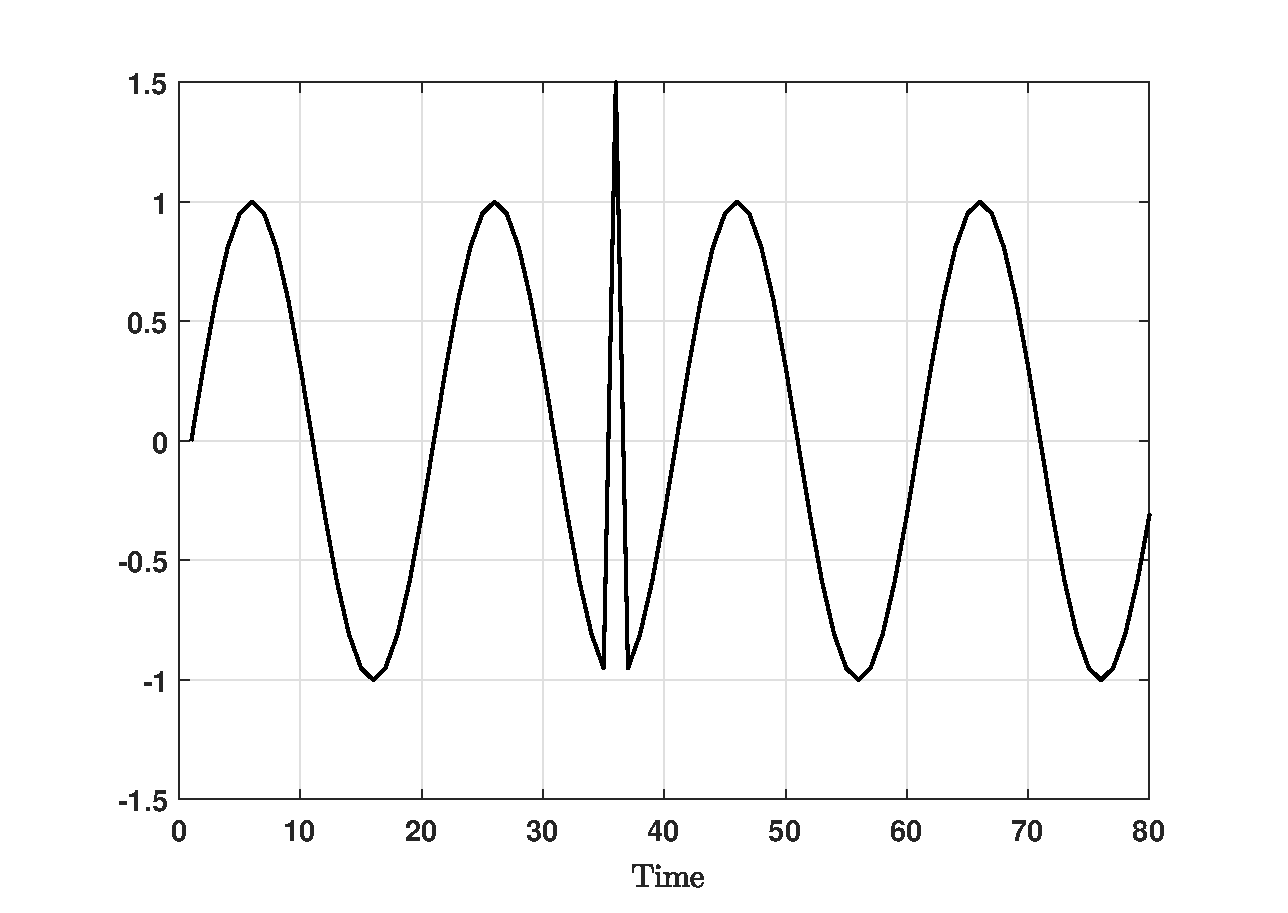
\includegraphics[scale=0.25]{introduction/Point_anomaly}
		\vspace{-0.5cm}
		\caption{Global point outlier.}
		\label{fig:intro_point}
	\end{minipage}
		\vspace{-0.15cm}
	\begin{minipage}{0.33\textwidth}
		\centering
		\includegraphics[scale=0.25]{introduction/Contextual_anomaly}
		\vspace{-0.5cm}
		\hspace{0.15cm}
		\caption{Contextual point outlier.}
		\label{fig:intro_contextual}
	\end{minipage}
		\vspace{-0.15cm}
	\begin{minipage}{0.33\textwidth}
		\centering
		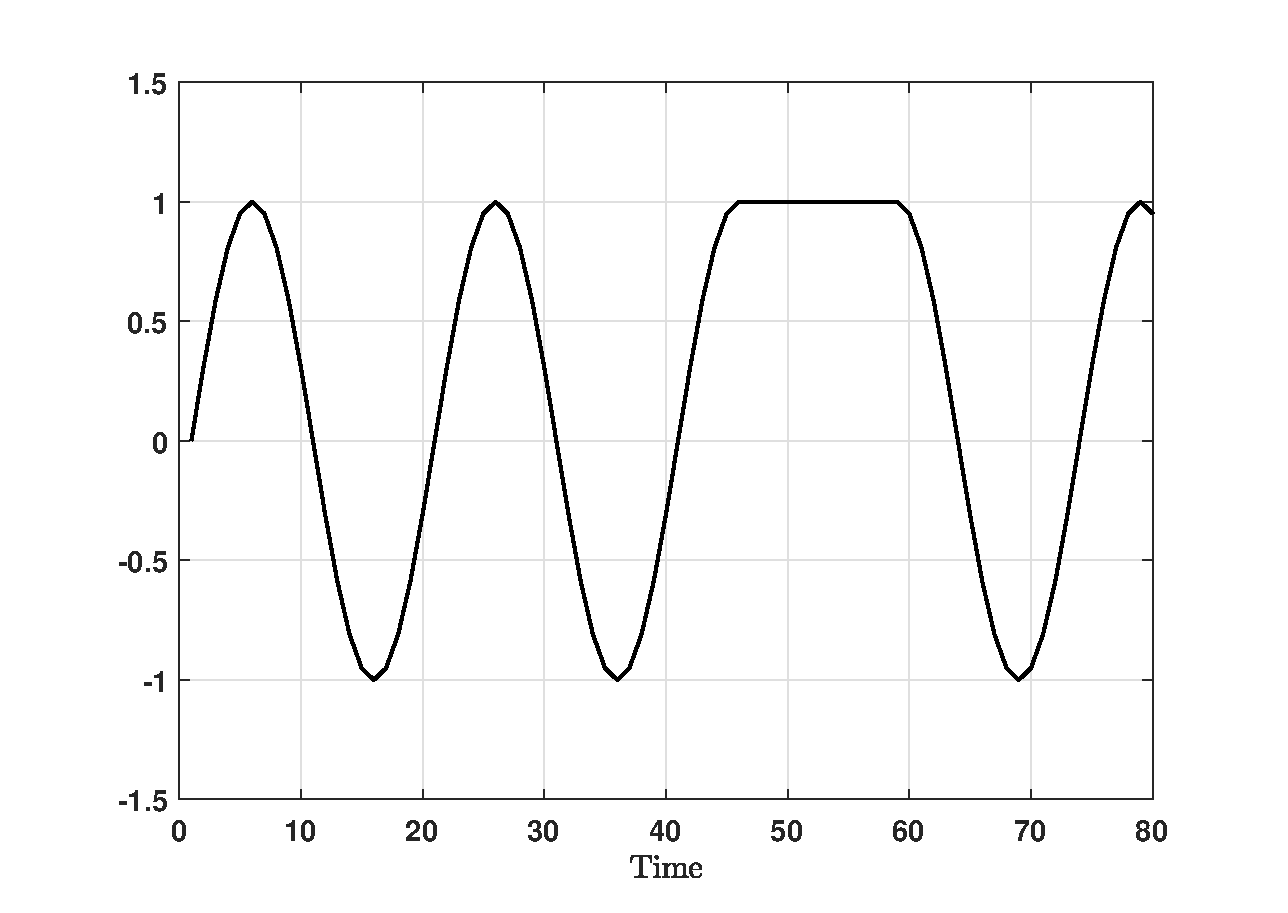
\includegraphics[scale=0.25]{introduction/Collective_anomaly}
		\vspace{-0.5cm}
		\hspace{-0.15cm}
		\caption{Collective outlier.}
		\label{fig:intro_collective}
	\end{minipage}
		\vspace{-0.15cm}
\end{figure}

\newpage
The second challenge associated with outlier detection in multivariate time series is to deal with the effect of the high dimensionality of the data points. Having more features describing each incoming data point might seem to yield a higher chance of observing data points that deviate significantly from what is considered normal. However, having more data at your disposal does not automatically mean that outliers can be separated better from normal data points. At some point, the dimensionality of a data set introduces problems which is often referred to as the curse of dimensionality. 

One problem is that the norms of data points in a data set $\mathbf{X}$ of high dimensionality $d$, for example, tend to approach the same value as the number of features goes to infinity \cite{zimek2012survey}. This means there is little variance between data points in $\mathbf{X}$ if we look at the ratio between the norms of the data points in $\mathbf{X}$ and the norm of the mean of $\mathbf{X}$. As a consequence, the largest distance between a pair of two data points in $\mathbf{X}$ 
approaches the smallest pair-wise distance 
\cite{beyer1999nearest}. This concentration of distances makes the difference between outlier scores associated with outliers and normal data points vanish. 

Another downside is the computational burden induced by processing high-dimensional data points. The main cause of computational issues lies in the search space imposed by an increasing dimensionality. That is, outliers are often characterized by deviating values in a subspace rather than in the full feature space. The consequence is that algorithms often search for meaningful subspaces in which outliers can be discriminated. An increase in the number of features $d$, therefore, implies an exponential growing search space \cite{zimek2012survey}. Going through all $(2^d - 1)$ possible subsets for $d$ features is considered not tractable if $d$ is high.

Table \ref{tab:intro_characteristics} summarizes the challenges associated with each characteristic of outlier detection in multivariate time series in an online and unsupervised manner.

\begin{table}[h]
	\centering
	\caption{Challenges associated with our task.}
	\label{tab:intro_characteristics}
	\begin{tabular}{p{0.3\linewidth} p{0.6\linewidth}}
		\toprule
		\textbf{Characteristic}	&	\textbf{Challenge} \\
		\midrule
		\multirow{8}{*}{Online classification \cite{ahmad2017unsupervised,aggarwal2015outlier}} & The algorithm must assign label $O_i$ to data point ${\mathbf x}_i$ before receiving ${\mathbf x_{i+1}}$.\\[0.12cm]
		& The algorithm should only exploit a limited history of the data to infer its model, and not require storage of the entire stream.\\[0.12cm]
		& The algorithm should run unsupervised, i.e. without the need of labelling data points or manually adapting parameters.\\[0.12cm]
		& The detection performance should be not too sensitive to the (fixed) parameters.\\
		\midrule 
		\multirow{3}{*}{Outlier detection in} & The analyst should have an idea of the expected, normal behaviour, and of the outliers desired to detect. \\[0.12cm]
		time series \cite{chandola2009anomaly}& The algorithm should be able to detect contextual outliers besides global outliers. \\
		\midrule
		\multirow{4}{*}{High-dimensional data \cite{zimek2012survey}} & The algorithm should be able to find outliers in high-dimensional data. \\[0.12cm]
		& Algorithms should scale well in computational complexity with increasing numbers of time series $d$ and data points $n$.\\
		\bottomrule
	\end{tabular}
\end{table}



\section{Unsupervised online methods}

As a consequence of the diverse challenges as described, many approaches to unsupervised online outlier detection in multivariate time series exist. In this section we discuss a few recently proposed methods, which can be categorized in proximity-based and model-based methods. The application considered and the outliers expected, often make a certain method more suitable than others. For a discussion of existing methods in relation to common applications of online outlier detection in time series we refer to the surveys by Gupta et al. \cite{gupta2014outlier} and Chandola et al. \cite{chandola2009anomaly}. 

\subsection{Related methods}
\label{sec:introduction_related}
Proximity-based methods examine the spatial proximity of data points to discriminate data points that significantly deviate from the proximity of the majority of data points. The proximity of an incoming data point is mostly reflected by a distance or density measure in context of its preceding data points.
A recently developed density-based method is Loda, short for light-weight online detector of anomalies\footnote{The term \textit{anomalies} is considered to refer to the same concept as \textit{outliers}.} \cite{pevny2016loda}. Loda projects the incoming data point into $k$ random $1$-dimensional subspaces and maintains $k$ histograms with $b$ bins to approximate a probability density function. The average of the log probability approximated by these $k$ histograms, is assigned to the data point as its outlier score. The histograms are constantly updated as new data points come in. 

A distance-based method suitable for online outlier detection in high-dimensional data streams is LEAP \cite{cao2014scalable}. LEAP slides a window of size $p$ over the data stream and computes the distance of an incoming data point $\mathbf{x}_i$ to data points within this window. It does so until there is minimal yet enough evidence that $\mathbf{x}_i$ is not an outlier. If the minimal evidence threshold is not exceeded, the entire neighbourhood of the data point is evaluated. This minimal evidence threshold is based on the distance between the incoming data point and a few prototype data points in its surrounding window. Such prototypes are selected over time, which implies that the total reference set evolves over time. A data point is flagged as an outlier if its distance to the prototypes, or to all data points in the current window exceed a threshold.

\vspace{0.1cm}

Model-based outlier detection methods describe the expected behaviour of the multivariate time series with a model. Various options exist for modelling the data online and use the resulting model to generate binary labels or outlier scores for incoming data points. Recently, Ahmad et al. \cite{ahmad2017unsupervised} proposed an unsupervised method that models the data online using Hierarchical Temporal Memory (HTM) networks. Such networks encode data points in a lower-dimensional subspace and represent it as a sparse binary vector. A so-called sequence memory component models the temporal patterns from these binary vectors and generates predictions for upcoming data points. A more detailed explanation of HTM networks can be found in \cite{cui2016continuous}. Ahmad et al. use this technique to infer outlier scores from the distribution of historic prediction errors generated by the HTM network.

A different model-based approach, principal component analysis (PCA), also represents the $d$ time series in a lower-dimensional subspace. It does so by linearly projecting the data into directions in which most of the variance in the data is captured \cite{jolliffe1986principal}. After projecting the data into this optimized subspace, the lower-dimensional representation is reconstructed to the original dimensionality $d$. The outliers are then hopefully not explained by the principal components, such that the distance between the original data points and their reconstructions yields a discriminative outlier measure. A well-known method to approximate the principal components unsupervised and online is SPIRIT \cite{papadimitriou2005streaming}. SPIRIT is considered to be a tractable and effective method for online outlier detection in multivariate time series \cite{aggarwal2015outlier}. As it has strong similarities with the method we propose, we explain this method in more detail in chapter \ref{chap:reconstruction-detection}. 

The methods discussed in this section are suitable for unsupervised online outlier detection in multivariate time series and considerably effective. Still, we think there is a promising direction left unexplored that introduces methods to solve this problem in a more efficient manner.


\subsection{The proposed method in a nutshell}
In this thesis we attempt to address the challenges as listed in table \ref{tab:intro_characteristics} with only one method: random projections. The proposed random projection method projects or maps data points of high dimensionality $d$ into a random $k$-dimensional subspace. If our mapping function $\mathbf{f}$ satisfies certain conditions, we are guaranteed that the obtained lower dimensional representation preserves the pair-wise Euclidean distances in our data stream ${\mathbf X}$ up to some error \cite{johnson1984extensions}. The obtained $k$-dimensional representation of a data point at time step $i$, $\mathbf{x}_i'$, is reconstructed back into the original dimensionality $d$. This reconstructed data point $\hat{\mathbf{x}}_i$ then functions as a model of the original data point $\mathbf{x}_i$. As this method does not update any projection directions or optimize mapping functions on the data, it is an efficient method.

The first proposed use of this method interprets the squared Euclidean distance between $\mathbf{x}_i$ and $\hat{\mathbf{x}}_i$ as the outlier score $O_i$ as in equation \eqref{eq:intro_squared_euclidean}. 

\begin{equation}\label{eq:intro_squared_euclidean}
	O_i =\left( \ \sqrt{\sum\limits_{j=1}^d (\mathbf{x}_{i,j} - \hat{\mathbf{x}}_{i,j})^2} \ \right)^2 = \sum\limits_{j=1}^d (\mathbf{x}_{i,j} - \hat{\mathbf{x}}_{i,j})^2
\end{equation}

\noindent Throughout the remainder of this thesis we represent this distance as $\|\mathbf{x}_i - \hat{\mathbf{x}}_i\|^2$. The conversion from this continuous score to a discrete label is considered beyond the scope of this thesis as the level of outlierness corresponding to an `actual' outlier likely depends on the system being observed.


Contextual outliers are particularly hard to detect with our method using this outlier measure. Therefore, we present an additional interpretation of the reconstructions obtained from random projections that enables detecting contextual outliers as well. This alternative is based on $2$ distinct runs of the random projection method with different values for the number of projection vectors $k$. We take the difference between the two obtained reconstructions as indicator of the outlierness at time step $i$. This method is explained in more detail in chapter \ref{chap:analysis}.

Projecting the data into random directions implies the projection is not optimized on the data at hand, and is therefore called data-independent. Beside its benefits for the runtime performance, a data-independent method also makes theoretical analysis of its properties possible. For example, the lower bound on the projection dimensionality $k$ only depends on the number of data points $n$, the choice for random mapping $\mathbf{f}$ and maximum distortion $\varepsilon$. This enables full control over the quality of the lower-dimensional representation as we can choose $\mathbf{f}$ and an acceptable distortion $\varepsilon$. In chapter \ref{chap:rp-method} we thoroughly explain the random projection method.

The question we focus on throughout this thesis is: \textit{can we leverage random projections in an online and unsupervised reconstruction-based method in order to find outliers in multivariate time series effectively though more efficiently, and if so, to what extent?} 
In particular, we investigate if and to what extent the method we propose defeats the challenges as summarized in table \ref{tab:intro_characteristics}.


\section{Outline of this thesis}

In this chapter, we have formulated the problem context and explained the challenges it imposes. We also provided an overview of related methods to conduct online outlier detection in multivariate time series, and briefly explained the proposed method. The remainder of this thesis is organized as follows. First, we explain the general approach of reconstruction-based outlier detection in more detail in chapter \ref{chap:reconstruction-detection}. We proceed in chapter \ref{chap:rp-method} with the formulation of the proposed random projection method. An analysis of this method on synthetic data follows in chapter \ref{chap:analysis}. Chapter \ref{chap:experiments} presents the results of experiments conducted with real-world time series data, where we also explore the applicability of the random projection method on non-temporal data sets. We conclude this thesis in chapter \ref{chap:discussion} with an overview of the key findings and conclusions, and suggestions for future work.



\chapter{Reconstruction-based outlier detection}
\label{chap:reconstruction-detection}

We explore the applicability of random projections in a reconstruction-based outlier detection method.
To that end, this chapter elaborates on reconstruction-based outlier detection in section \ref{sec:reconstruction_mappings} and zooms in on two such approaches in section \ref{sec:reconstruction_methods}. In section \ref{sec:reconstruction_spirit} we explain one method in detail as it is taken as a baseline for comparisons. We conclude with summarizing the open challenges that are taken as objectives for our method in section \ref{sec:reconstruction_challenges}.

\section{Mappings, reconstructions and outlier scores}
\label{sec:reconstruction_mappings}

In practice, classes might be better distinguishable in a high-dimensional feature space if the underlying data of interest is oriented in a subspace of lower dimensionality than it is originally \cite{beyer1999nearest}. Hence, it is assumed we can capture, or model, the data in a lower-dimensional representation and find a suitable way to reconstruct this model to a higher-dimensional representation. This reconstruction then hopefully approximates the normal behaviour in the original dimensionality such that outliers significantly deviate from it. We can obtain a $k$-dimensional representation by

\begin{equation}\label{eq:reconstruction_projection}
\mathbf{x}' = \mathbf{f}(\mathbf{x})
\end{equation}  

\noindent with mapping function $\mathbf{f} : \mathbb{R}^d \to \mathbb{R}^k$ ($k \ll d$) and $\mathbf{x}$ a vector of size $d \times 1$. Then, this mapping $\mathbf{x}'$ of size $k \times 1$ can be reconstructed to its original dimensionality $d$ using

\begin{equation}\label{eq:reconstruction_reconstruction}
\hat{\mathbf{x}} = \mathbf{g}(\mathbf{x}')
\end{equation}  

\noindent with $\mathbf{g} : \mathbb{R}^k \to \mathbb{R}^d$. Hopefully, reconstruction $\hat{\mathbf{x}}$ represents $\mathbf{x}$ as if it belongs to the class of normal data points. If $\mathbf{x}$ actually belongs to the class of outliers, $\mathbf{x}$ and $\hat{\mathbf{x}}$ would significantly differ from each other. This difference can be taken as the outlier score such that large differences represent the outliers. We could, for instance, take the squared Euclidean distance between the reconstruction and the original data point such that

\begin{equation}\label{eq:reconstruction_score}
 O = \|\mathbf{x} - \hat{\mathbf{x}}\|^2.
\end{equation}  

The squared Euclidean distance between $\mathbf{x}$ and $\hat{\mathbf{x}}$ emphasizes large differences between $\mathbf{x}$ and $\hat{\mathbf{x}}$. Therefore, this distance measure is considered an appropriate indicator of the outlierness of $\mathbf{x}$.
To obtain a final label of $\mathbf{x}$, a threshold $\theta$ is needed. Data points associated with outlier scores exceeding that threshold, i.e. $O > \theta$, are labelled as outliers. Evidently, it depends on the application itself and the desired balance between false and true detections what to take for $\theta$. Therefore we do not focus on finding a procedure to derive $\theta$.

Fitting this general reconstruction-based approach within the context of online outlier detection methods for multivariate time series, we can illustrate the detection procedure as in figure \ref{fig:reconstruction_reconstruction}.

\begin{figure}[h]
	\centering
	\vspace{0.25cm}
	\includegraphics[scale=0.85]{reconstruction-detection/reconstruction_outlierdetection_noexp}
	\caption{General process of reconstruction-based unsupervised online outlier detection in multivariate time series.}
	\label{fig:reconstruction_reconstruction}
\end{figure}

\newpage
\section{Reconstruction-based outlier detection methods}
\label{sec:reconstruction_methods}

A well-known reconstruction-based outlier detection approach, principal component analysis (PCA), learns a linear projection in $k$ orthogonal directions that together capture a large fraction of the variance in the data. Alternative artificial neural networks (ANN) can be used, which typically result in nonlinear functions $\mathbf{f}$ and $\mathbf{g}$ that explicitly minimize the mean squared error. 

\subsection{Principal component analysis}

The basic assumption of PCA, is that our $d$ features likely exhibit linear correlations among each other \cite{aggarwal2015outlier}. If so, we can represent the original $d$-dimensional feature space using only $k$ uncorrelated variables where $k \ll d$. In general, if $\mathbf{X}$ exhibits substantial correlations among the different time series, the first principal components will already explain most of the variation in the original time series \cite{jolliffe1986principal}. The last components will then explain the directions in which only little variation exists and, therefore, probably align well with the outliers we look for.

Outliers in time series are not necessarily characterized by extreme values in any of the original features. Instead, using principal component analysis we can also find outliers that do not conform with the temporal pattern of the remainder of the data. Logically, the analyst is in charge of making an educated guess of the amount of variance needed to explain. Therefore, the number of components $k$ needed to capture the principal temporal patterns should be estimated properly on forehand such that the outliers in $\mathbf{X}$ are not modelled too.

Starting from this intuition, PCA obtains the $k$ principal projection directions by concentrating on an orthonormal linear subspace that maximizes the variance explained in the data. More specifically, it optimizes the $k$ projection directions such that they align with the $k$ (ordered) largest eigenvalues of the covariance matrix of $\mathbf{X}$. For a detailed overview of possible optimization procedures to obtain the projection with PCA, we refer to the work of Jolliffe \cite{jolliffe1986principal}. 

Figure \ref{fig:reconstruction_geometry_projections} illustrates how projecting three data points \{$\mathbf{x}_i : i = 1,2,3$\} in the first principal direction (right), retains the most variance in a $1$-dimensional subspace compared to projecting simply on the y- or x-axis (respectively left and center). 

\begin{figure}[!h]
	\centering
	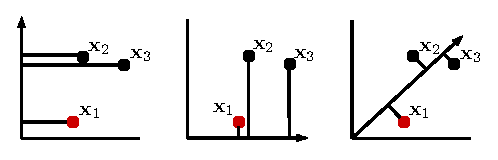
\includegraphics[scale=1.8]{reconstruction-detection/geometry_projections_pca1}
	\caption{Geometric visualization of projections onto the y-axis (left), x-axis (center) and principal direction (right).}
	\label{fig:reconstruction_geometry_projections}
\end{figure}

\newpage
However, in this particular $2$-dimensional case, taking the first principal direction as a model for reconstruction to the original dimensionality might not yield a good base for discriminating outliers. That is, from this projection we expect a good reconstruction of the data point $\mathbf{x}_1$, which could be considered an outlier looking at $\mathbf{x}_2$ and $\mathbf{x}_3$ only. This example reflects the main risk of the PCA-based reconstruction method for outlier detection: if the outliers can be separated well from the principal components used to model the principal behaviour, we can reconstruct our outliers properly resulting in low reconstruction errors and thus low outlier scores. The latter is obviously not what we wish for. 

Clearly, if we extend this example to a feature space with $d \gg 2$, it is crucial to choose the number of projection vectors $k$ carefully in order to make PCA not fit to the outliers. Obtaining a proper $k$-dimensional representation, then, hopefully enables us to separate the outliers by concentrating at data points with the highest reconstruction errors. 

As PCA results in linear projections of the data, $\mathbf{f}$ and $\mathbf{g}$ represent simple matrix multiplications. The projection $\mathbf{x}'$ of $\mathbf{x}$ is obtained from a simple multiplication with all $k$ principal coefficient vectors $\mathbf{w} \in \mathbf{W}$, i.e.

\begin{equation}\label{eq:reconstruction_pcaprojection}
\mathbf{x}' = \mathbf{W} \ \mathbf{x}
\end{equation}

\noindent where $\mathbf{W}$ is called the principal coefficient matrix of size $k \times d$. Then the projected data point $\mathbf{x}'$ can easily be reconstructed to its original dimensionality $d$ using

\begin{equation}\label{eq:reconstruction_pcareconstruction}
\hat{\mathbf{x}} = \mathbf{W}^T \ \mathbf{x}'
\end{equation}  

\noindent taking the transpose $\mathbf{W}^T$ instead of the inverse $\mathbf{W}^{-1}$. We can reconstruct $\mathbf{x}'$ accurately this way, as all $\mathbf{w} \in \mathbf{W}$ are orthogonal to each other and have unit length. That is, we have

\begin{equation}\label{eq:reconstruction_orthonormality}
\mathbf{W}^T \ \mathbf{W} = \mathbf{I}
\end{equation}

\noindent with $\mathbf{I}$ the identity matrix, which is a sufficient condition for accurate reconstruction\footnote{In case the first $k$ components explain the majority of the variance in the data.} using $\mathbf{W}^T$. Outlier scores can be computed as in equation \eqref{eq:reconstruction_score}. A method to conduct approximate principal component analysis online and unsupervised is discussed in section \ref{sec:reconstruction_spirit}. 
 
\vspace{0.2cm}
\subsection{Artificial neural networks}
In some cases, it is infeasible to accurately represent the normal behaviour in a linear lower-dimensional subspace. For those cases, we can resort to nonlinear mappings of the data instead. The objective is to learn a nonlinear function $\mathbf{f} : \mathbb{R}^d \to \mathbb{R}^k$ such that, in turn, the data can be reconstructed by a function $\mathbf{g} : \mathbb{R}^k \to \mathbb{R}^d$. These functions are usually obtained by training an artificial neural network (ANN) on data such that the combination of the two minimize, for example, the mean squared error as in equation \eqref{eq:reconstruction_ann}. 

\begin{equation}\label{eq:reconstruction_ann}
\min_{\mathbf{f},\ \mathbf{g}}\frac{1}{d}\sum\limits_{j=1}^{d}(\mathbf{x}_{j} - \mathbf{g}(\mathbf{f}(\mathbf{x}_{j})))^2
\end{equation}

ANN's are inspired on biological processes taking place in brains to learn representing and reproducing real-world phenomena accurately. Each neuron, or node, in an ANN typically processes its received input (the initial input, or the output of a previous layer) and transmits it to a node in the next layer. Eventually, the ANN is trained to approximate the input by learning its underlying characteristics. Well-known approaches that learn functions $\mathbf{f}$ and $\mathbf{g}$ this way, are autoencoder networks \cite{japkowicz1995novelty} and the multi-layer perceptron \cite{nairac1999system}.

For unsupervised online outlier detection in time series, a recently proposed method combines autoencoders with the principle of variational inference \cite{solch2016variational}. This principle relates to replacing the lower-dimensional encoding $\mathbf{x}'$ of $\mathbf{x}$, and corresponding decoding $\hat{\mathbf{x}}$, with approximations of posterior distributions represented by stochastic variables. The parameters of these stochastic variables are, in turn, learned by recurrent neural networks which capture the temporal dynamics of the time series online.

\newpage
\section{Baseline: online principal component approximation}
\label{sec:reconstruction_spirit}
Though the data at hand might be structured nonlinearly, in this thesis we focus on linear projections of the data. Therefore, we compare the obtained performances to a method approximating the (linear) principal coefficient vectors online, called SPIRIT \cite{papadimitriou2005streaming}. 
Instead of learning the coefficient vectors $\mathbf{w} \in \mathbf{W}$ offline, SPIRIT updates $\mathbf{W}_i$ each time step $i$ to approximate the optimal $k$ orthogonal directions in which the explained variance is maximized. Algorithm \ref{alg:trackw} gives a detailed insight of how the $k$ coefficient vectors are updated over time\footnote{Algorithm \ref{alg:trackw} represents only the update of the projection vectors of the actual algorithm of SPIRIT.}.

In short, the $k$ vectors are updated proportionally to the reconstruction error (step \ref{alg:trackw_op6}) associated with the projection $\mathbf{x}_i'$ onto the $k$ projection vectors at time step $i$ (step \ref{alg:trackw_op4}). The impact of each incoming data point on the updated projection vectors is controlled by a so-called forgetting factor $\lambda$ (steps \ref{alg:trackw_op5} and \ref{alg:trackw_op7}). If $\lambda$ is close to $1$, recent data points have less significant effect on the updates. This way, temporal relations are tracked over time. A suitable range for $\lambda$ to make SPIRIT generalize well to a broad range of applications is [$0.96$, $0.98$] \cite{papadimitriou2005streaming}. 

\begin{algorithm}[H]
	\caption{\quad \textbf{TrackW}}
	\label{alg:trackw}
	\begin{algorithmic}[1]
		\STATE Initialize $k$ coefficient vectors $\mathbf{w}_j$ to unit vectors s.t. $\mathbf{w}_1 = [10\cdots0]$, $\mathbf{w}_2 = [010\cdots0]$, etc. \label{alg:trackw_op1}
		\STATE Initialize $\tilde{\mathbf{x}}_j$ as $\mathbf{x}_i$ \label{alg:trackw_op2}
		\STATE Initialize $d_1$ to a small value between $0$ and $1$
		\label{alg:trackw_op3}
		\FOR{$1 \leq j \leq k$}
		\STATE Project $\tilde{\mathbf{x}}_j$ on $\mathbf{w}_j$ by $x_j' = \mathbf{w}_j \ \tilde{\mathbf{x}}_j$
		\label{alg:trackw_op4}
		\STATE Update $d_j \gets \lambda d_j + (x_j')^2$ \qquad\quad \ \COMMENT{Energy $\propto$ $j$th eigenvalue of $\mathbf{X}_i^T\mathbf{X}_i$}
		\label{alg:trackw_op5}
		\STATE Set $\mathbf{e}_j = \tilde{\mathbf{x}}_j - x_j' \mathbf{w}_j^T $ 
		\label{alg:trackw_op6}
		\STATE Update $\mathbf{w}_j \gets \mathbf{w}_j + \frac{1}{d_j} \ x_j' \ \mathbf{e}_j$ \qquad \COMMENT{Update principal coefficients estimate}
		\label{alg:trackw_op7}
		\STATE $\tilde{\mathbf{x}}_{j+1} \gets \tilde{\mathbf{x}}_j - x_j' \ \mathbf{w}_j^T$
		\label{alg:trackw_op8}
		\ENDFOR
	\end{algorithmic}
\end{algorithm}

Figure \ref{fig:reconstruction_updatew} illustrates the procedure of updating the principal projection directions as soon as a new data point arrives.

\begin{figure}[h]
	\centering
	\vspace{-0.12cm}
	\includegraphics[scale=1]{reconstruction-detection/SPIRIT_updateW}
	\caption{Update procedure of the first estimated principal coefficient vector $\mathbf{w}_1$ for new data point $\mathbf{x}_i$ (in red).}
	\label{fig:reconstruction_updatew}
\end{figure}

Algorithm \ref{alg:spirit} describes the full procedure of how SPIRIT detects outliers in multivariate time series.
Aside from the projection directions, the number of vectors needed to explain the amount of variance as requested by the analyst is updated over time as well\footnote{Technically, the explained variance is estimated. Therefore, this estimated variance is referred to as the `retained energy' of the $k$ coefficient vectors $\mathbf{w} \in \mathbf{W}_i$ denoted by $E_{tot}$.}. SPIRIT takes the bounds reflecting the desired variance to retain as input, which are referred to as $f_{\hat{E}}$ being the lower variance bound and $F_{\hat{E}}$ as the upper variance bound. The variance explained with the $k$ projection vectors at time step $i$ are estimated (step \ref{alg:spirit_op7}), and compared with the provided variance bounds. If the estimated explained variance is lower than these bounds, an additional projection vector is added (\ref{alg:spirit_op8} to \ref{alg:spirit_op10}). If the estimated explained variance is higher than these bounds, the last vector is removed (steps \ref{alg:spirit_op11} to \ref{alg:spirit_op13}).

\vspace{-0.2cm}
\begin{algorithm}[H]
	\vspace{-0.02cm}
	\caption{\quad \textbf{SPIRIT}}
	\label{alg:spirit}
	\vspace{-0.03cm}
	\begin{algorithmic}[1]
		\vspace{-0.025cm}
		\STATE Initialize $k \gets 1$, $E \gets 0$ and $\hat{\mathbf{E}}_1 \gets 0$
		\FOR{${\mathbf x}_i \in {\mathbf X}$}
		\STATE Project $\mathbf{x}_i$ on $\mathbf{W}_i$ by $\mathbf{x}_i' = \mathbf{W}_i \ \mathbf{x}_i$
		\STATE	Set $O_i = \|\mathbf{x}_i - \mathbf{W}_i^T \ \mathbf{x}_i'\|^2$
		\label{alg:spirit_op4}	
		\STATE Update $\mathbf{w}_j \in \mathbf{W}_i$ for $1 \leq j \leq k$ by starting at step \ref{alg:trackw_op2} of algorithm \ref{alg:trackw} 
		\label{alg:spirit_op3}
		\STATE Set $E \gets \frac{(i - 1)E + \|\mathbf{x}_i\|^2}{i}$
		\label{alg:spirit_op5}
		\STATE Update $\hat{\mathbf{E}}_j \gets \frac{(i - 1)\hat{\mathbf{E}}_j + (\mathbf{x}_{i,j}')^2}{i}$ for $1 \leq j \leq k$
		\label{alg:spirit_op6}
		\STATE Estimate retained energy $\hat{E}_{tot} \gets \sum\limits_{j=1}^{k}\hat{\mathbf{E}}_j$
		\label{alg:spirit_op7}
		\IF{$\hat{E}_{tot} < f_{\hat{E}} \ E$}
		\label{alg:spirit_op8}
		\STATE Set $k \gets k + 1$ and $\hat{\mathbf{E}}_{k+1} \gets 0 $
		\label{alg:spirit_op9}
		\STATE add $\mathbf{w}_{k+1}$ to $\mathbf{W}_i$ by starting at step \ref{alg:trackw_op1} of algorithm \ref{alg:trackw}
		\label{alg:spirit_op10}
		\ELSIF{$\hat{E}_{tot} > F_{\hat{E}} \ E$}
		\label{alg:spirit_op11}
		\STATE Set $k \gets k - 1$
		\label{alg:spirit_op12}
		\STATE discard $\mathbf{w}_k$ and $\hat{\mathbf{E}}_k$
		\label{alg:spirit_op13}
		\ENDIF
		\ENDFOR
	\vspace{-0.02cm}	
	\end{algorithmic}
\vspace{-0.1cm}
\end{algorithm}

\vspace{-0.1cm}
The computational complexity of algorithm \ref{alg:spirit} (for each time step $i$) is expressed as $\mathcal{O}(kd)$ \cite{papadimitriou2005streaming}. This means that its runtime mainly depends linearly on the number of components needed to explain the desired fraction of variance between $f_{\hat{E}}$ and $F_{\hat{E}}$, and the number of data points $n$. 
However, though not explicitly included in algorithm \ref{alg:spirit}, the implementation of the algorithm distributed by the authors includes an orthogonalization procedure to obtain an orthonormal $\mathbf{W}_i$ after step \ref{alg:spirit_op3}. Experiments ran without the Gram-Schmidt orthogonalization procedure pointed out we indeed need a strictly orthonormal projection basis $\mathbf{W}_i$ to obtain a good performance for outlier detection purposes. Unfortunately, the need for orthogonalizing $\mathbf{W}_i$ results in a runtime of $\mathcal{O}(k^2d)$ which might be costly if $d$ or $k$ is high. 

Despite the need of orthogonalizing the projection vectors, we selected SPIRIT as a baseline as it is considered tractable for online outlier detection in multivariate time series \cite{aggarwal2015outlier}. Additionally, it runs online without the need for a training phase (supervision). Finally, though not directly a motivation for using SPIRIT as a baseline, taking a linear reconstruction-based method as a baseline makes the intuition behind and understanding of our proposed method easier.

\vspace{-0.1cm}
\section{Open challenges}
\label{sec:reconstruction_challenges}
In this chapter we discussed reconstruction-based outlier detection and identified a few vulnerabilities of such methods, in particular of SPIRIT. Now it is time to make those vulnerabilities more explicit, as they directly led us to the formulation of the objectives of our method.

In figure \ref{fig:reconstruction_geometry_projections}, we illustrated a projection of three data points aligned with the principal direction of those data points. In situations like this one, we would reconstruct our outliers accurately which is the undesired result of using the reconstruction from lower-dimensional representations for outlier detection. 
If we would know the appropriate number of projection vectors to explain the variance of the normal behaviour only, without fitting to the outliers as well, we can count on a good detection performance. However, it is hard to determine variance bounds that generalize well to unseen data streams. Besides, SPIRIT is supposed to run unsupervised, making it impossible to adjust these bounds online. This last resort would also not help for cases where the system behaviour is non-stationary, as one has to adjust these bounds constantly. In general online unsupervised (reconstruction-based) methods for outlier detection are sensitive to parameter settings \cite{aggarwal2015outlier}, introducing the objective to find a method that defeats that challenge for unsupervised online outlier detection. 

Finally, we discussed that SPIRIT in practice might result in a poor computational performance. Going from our problem formulation, we operate in high-dimensional feature spaces for which SPIRIT might not be tractable after all. Especially for outlier detection purposes, we need $\mathbf{W}_i$ to be a strictly orthonormal projection basis, making a costly orthogonalization procedure indispensable. Our second objective regarding the formulated challenges in \ref{tab:intro_characteristics}, therefore, is to improve the runtime performance of $\mathcal{O}(k^2d)$ per time step.



\chapter{The random projection method}
\label{chap:rp-method}

In this chapter we present the proposed method in detail and discuss its constructive elements. First, we explain the central idea behind our proposal in section \ref{sec:method_idea} and provide a brief overview of the theory behind random projections. In section \ref{sec:method_elements}, we proceed with a study of the critical elements that together compose the random projection method for reconstruction-based outlier detection. We conclude with the final formulation of the method in section \ref{sec:method_formulation}.

\section{Making use of random projections}
\label{sec:method_idea}
In this section we go through the main idea behind our method and discuss the lemma standing at the basis of our hypothesis. We also explain the variants of methods to generate random projection directions as found in the literature, and which variant we implement.

\subsection{The idea}
As already explained in the previous chapters, the PCA-based reconstruction method for outlier detection is closely related to our method. More specifically, instead of projecting the data into the principal directions and make all computational efforts to obtain those directions online, we simply project the data in random directions and hope for the best. 

Obviously, projecting the data into random directions takes away the computational burden associated with outlier detection methods based on PCA or other data-dependent methods. Another beneficial property is that we only need to set one parameter: the number of projection vectors $k$. With these two properties of random projections, we attempt to address the two main shortcomings of SPIRIT in the light of the challenges. Figure \ref{fig:method_geometry_rp} illustrates the geometrical difference between projecting the data into the (first) principal direction and a random direction. 

\begin{figure}[h]
	\centering
	\includegraphics[scale=1.8]{rp-method/geometry_projections_rp1}
	\caption{Geometrical representation of a projection into the first principal (left) and a random direction (right).}
	\label{fig:method_geometry_rp}
\end{figure}

This random model likely enables reconstruction of the outliers to some extent, but the squared Euclidean distance between a reconstructed outlier and its original version is still assumed to be higher than for the normal data points. Therefore, we hypothesize that a less perfect model than resulting from the principal components might still be sufficient in order to interpret the reconstruction errors as outlier scores. It might be the case, that we need more random projection vectors to obtain a reasonable model that approaches the model obtained by PCA-based methods. Hypothesis \ref{hyp:method_foundation} formulates this idea more formally.

\vspace{0.2cm}
\begin{hypothesis}\label{hyp:method_foundation}
	Replacing the $k_{\text{pca}}$ principal coefficient vectors with $k_{\text{rp}}$ random coefficient vectors, where $k_{\text{pca}} < k_{\text{rp}}$, yields a similar model of the normal behaviour at a lower computational cost.
\end{hypothesis}
\vspace{0.2cm}

The principle underlying our idea is a lemma posed by Johnson and Lindenstrauss in 1984 \cite{johnson1984extensions}. They state that, given a data set $\mathbf{X}$ of size $d \times n$ there exists a linear mapping $\mathbf{f}$ to obtain a $k$-dimensional representation of $\mathbf{X}$ with $k \ll d$, such that with high probability the pair-wise (squared) Euclidean distances are preserved with distortion at most $\varepsilon$. See also lemma \ref{lemma:onelemma}.

\vspace{0.2cm}
\begin{lemma}\label{lemma:onelemma}
	(Johnson and Lindenstrauss \cite{johnson1984extensions}). Given $\varepsilon > 0$ and an integer $n$, let $k$ be a positive constant $k \geq \mathcal{O}(\frac{1}{\varepsilon^2}\log(n))$. Then, for an arbitrary data set ${\mathbf X}$ of $n$ data points ${\mathbf x} \in \mathbb{R}^d$, there exists an $\mathbf{f}$ : ${\mathbb R}^d \rightarrow {\mathbb R}^k$ such that for all pairs ${\mathbf x}, {\mathbf y} \in {\mathbf X}$:
	\[(1-\varepsilon)\|{\mathbf x} - {\mathbf y}\|^2 \leq \|\mathbf{f}({\mathbf x}) - \mathbf{f}({\mathbf y})\|^2 \leq (1+\varepsilon)\|{\mathbf x} - {\mathbf y}\|^2 \]
	with probability $1-\frac{1}{n^2}$.
\end{lemma}
\vspace{0.2cm}

Note that the projection dimensionality $k$ only depends on the number of data points $n$ in $\mathbf{X}$ and the allowed distortion $\varepsilon$, and not on the original dimensionality $d$. For example, if we want to represent $n=500$ data points in $\mathbb{R}^d$ with at most $\varepsilon = 0.1$ distortion we would need $k$ to be approximately $\frac{2}{0.1^2}\log(n) \approx 540$ according to the bound empirically found sufficient for most variants of $\mathbf{f}$ by Venkatasubramanian et al. \cite{venkatasubramanian2011johnson}. This implies that, irrespective of the original dimensionality $d$, we can represent all $500$ data points in a $540$-dimensional subspace while retaining the pair-wise distances properly. Obviously, this would only make sense if $d > 540$. 

The topic of what we can and should use for $\mathbf{f}$ has been studied a lot over the past years since dealing with high-dimensional data sets has received increasing interest as emphasized already in chapter \ref{chap:introduction}.
The most important work has been devoted to finding suitable mappings that reduce the presented lower bound on $k$, or to improve the computational effort associated with it. 

\vspace{0.3cm}
\subsection{Variants of $\mathbf{f}(\mathbf{x})$}

In the literature a large variation of methods can be found for obtaining a lower-dimensional representation of $\mathbf{X}$ using random projections, here we briefly present the most important developments. As mapping $\mathbf{f}$ is linear, we define it as a random matrix $\mathbf{R}$ and refer to it as the random projection matrix representing this mapping. Then, we can define $\mathbf{f}(\mathbf{x})$ by the matrix multiplication

\vspace{0.1cm}
\begin{equation}
	\mathbf{f}(\mathbf{x}) = \mathbf{R}\mathbf{x}.
\end{equation}

Johnson and Lindenstrauss initialized the study to random projections and proposed a first method for obtaining $\mathbf{R}$. They sampled each entry $r$ of $\mathbf{R}$ from the Gaussian distribution with $0$ mean and unit variance, i.e. $r \sim \mathcal{N}(0,1)$. The resulting projection matrix should then be orthogonalized to meet the conditions they found to be necessary:

\begin{itemize}
	\item Spherical symmetry: For any orthogonal matrix $\mathbf{X} \in \mathbb{R}^{d \times n}$, the entries in $\mathbf{R} \mathbf{X}$ and $\mathbf{R}$ follow the same distribution.
	\item Orthogonality: All $k$ projection vectors in $\mathbf{R}$ are orthogonal to each other.
	\item Normality: All $k$ projection vectors in $\mathbf{R}$ are of unit length \cite{ailon2009fast}.
\end{itemize}

Random projections are particularly useful if we want to avoid the computational burden of obtaining a qualitative lower-dimensional representation of a data set $\mathbf{X}$. Instead of optimizing this lower-dimensional representation, by making use of random projections we obtain a representation that solely preserves pair-wise distances, yet in a more efficient manner. Therefore, the need for orthogonalizing $\mathbf{R}$ is considered a bottleneck, especially if $d$ is high. Indyk and Motwani \cite{indyk1998approximate} significantly improved the computational complexity by drawing the entries $r$ of $\mathbf{R}$ from a normal distribution with $0$ mean and $\frac{1}{d}$ variance, which is equivalent to scaling a matrix $\mathbf{R}$ with $r \sim \mathcal{N}(0,1)$ with $\frac{1}{\sqrt{d}}$. Scaling $\mathbf{R}$ this way makes it orthonormal on expectation. The higher $d$ gets, the closer the resulting projection matrix approaches orthonormality. Technically speaking, $\mathbf{R}$ is only a projection matrix if it is strictly orthogonal, which obviously is not the case if it is orthogonal on expectation. For the sake of simplicity we ignore this for the remainder of this work, and slightly abuse terminology by referring to this approximately orthogonal linear mapping as an approximately orthogonal linear projection.

\vspace{0.2cm}
Following the desire of relaxing the necessity conditions for $\mathbf{R}$ as posed by Johnson and Lindenstrauss, Achlioptas \cite{achlioptas2003database} noticed that the spherical symmetry condition of $\mathbf{R}$ could be dropped as well. Instead of sampling all entries from Gaussian distributions resulting in dense but spherical symmetric projection matrices, we might as well sample from the simple distribution $\{-1,+1\}$ where each element is drawn equally likely. The operations needed to project $\mathbf{X}$ onto $\mathbf{R}$ then solely consist of summations and subtractions, which speeds up the computations. Another significant contribution by Achlioptas is the proposal of sampling the entries from a sparse distribution $\{-1,0,+1\}$. In that case, we can store $\mathbf{R}$ as a sparse matrix saving storage, where the number of operations needed to be done to project data points would be reduced at the same time. 

Several improvements and (advanced) alternatives for $\mathbf{R}$ followed \cite{li2006very,ailon2009fast,krahmer2011new,clarkson2013low}, resulting in even lower storage requirements, less projection vectors required or mathematical operations needed.
It depends on the structure of the data set at hand whether such more efficient (possibly sparse) random projection methods properly preserve its pair-wise distances. For example, if the data set is sparse, a sparse random projection matrix might not properly preserve pair-wise distances \cite{venkatasubramanian2011johnson}. 

\vspace{0.2cm}
\section{Fundamental building blocks}
\label{sec:method_elements}

As we do not assume a certain structure on the data stream, we simply adopted the conventional dense Gaussian version for $\mathbf{R}$ with entries $r \sim \mathcal{N}(0,1)$ which was shown to be suitable for differently structured data sets. To bypass the expensive orthogonalization procedure, we scale our matrix as proposed by Indyk and Motwani \cite{indyk1998approximate}. 
Even though it often is not made explicit, it is important to scale the resulting projection with an additional factor $\sqrt{\frac{d}{k}}$ if one is concerned with preserving the original pair-wise Euclidean distances \cite{bingham2001random}. The reason behind this, is that the norms of the projections are down-scaled to $\sqrt{\frac{k}{d}}\|\mathbf{x}_i\|$ on expectation. To compensate for this effect, we could project $\mathbf{x}_i$ following

\vspace{0.1cm}
\begin{equation}\label{method_scaled_projection}
	\mathbf{x}_i' = \sqrt{\frac{d}{k}} \frac{1}{\sqrt{d}} \mathbf{R} \mathbf{x}_i.
\end{equation}
\vspace{0.1cm}

It is not hard to imagine that we could simplify this by scaling $\mathbf{R}$ directly with $\frac{1}{\sqrt{k}}$, which indeed seems to be a nice short-cut. The use of this short-cut as being interchangeable with the scaling factors used in equation \eqref{method_scaled_projection} can be found scattered throughout the literature \cite{arriaga1999algorithmic,achlioptas2003database,fradkin2003experiments}. Aside from the literature, this scaling method is frequently implemented by default in toolboxes such as scikit-learn \cite{scikit2018random}. We could blindly adopt this short-cut scaling method, but the success of our reconstruction-based method strongly coheres with the way projection matrix $\mathbf{R}$ is constructed. It also seems important to question to what extent we can use a projection matrix that is only orthonormal on expectation in order to use the cheap reconstruction method as in equation \eqref{eq:reconstruction_pcareconstruction}.

To evaluate these aspects of our method, we started investigating both scaling options to see if, and how well, they preserve the pair-wise Euclidean distances compared to a strictly orthonormal projection basis. To do so, we used a random data set of size $n = 997$ by $d = 300$. Figure \ref{fig:distortion_distances} shows how both scaling methods evidently result in the same distortion fraction of the pair-wise Euclidean distances. In addition, it can be seen that this data set could be qualitatively represented in a subspace of lower dimensionality than empirically found sufficient for most data sets as in \cite{venkatasubramanian2011johnson}. Finally, from this figure we can conclude that both scaling methods approach the distortion of the pair-wise distances as resulting from the strictly orthogonal projection matrix. 

\begin{figure}[h]
	\centering
	\vspace{-0.1cm}
	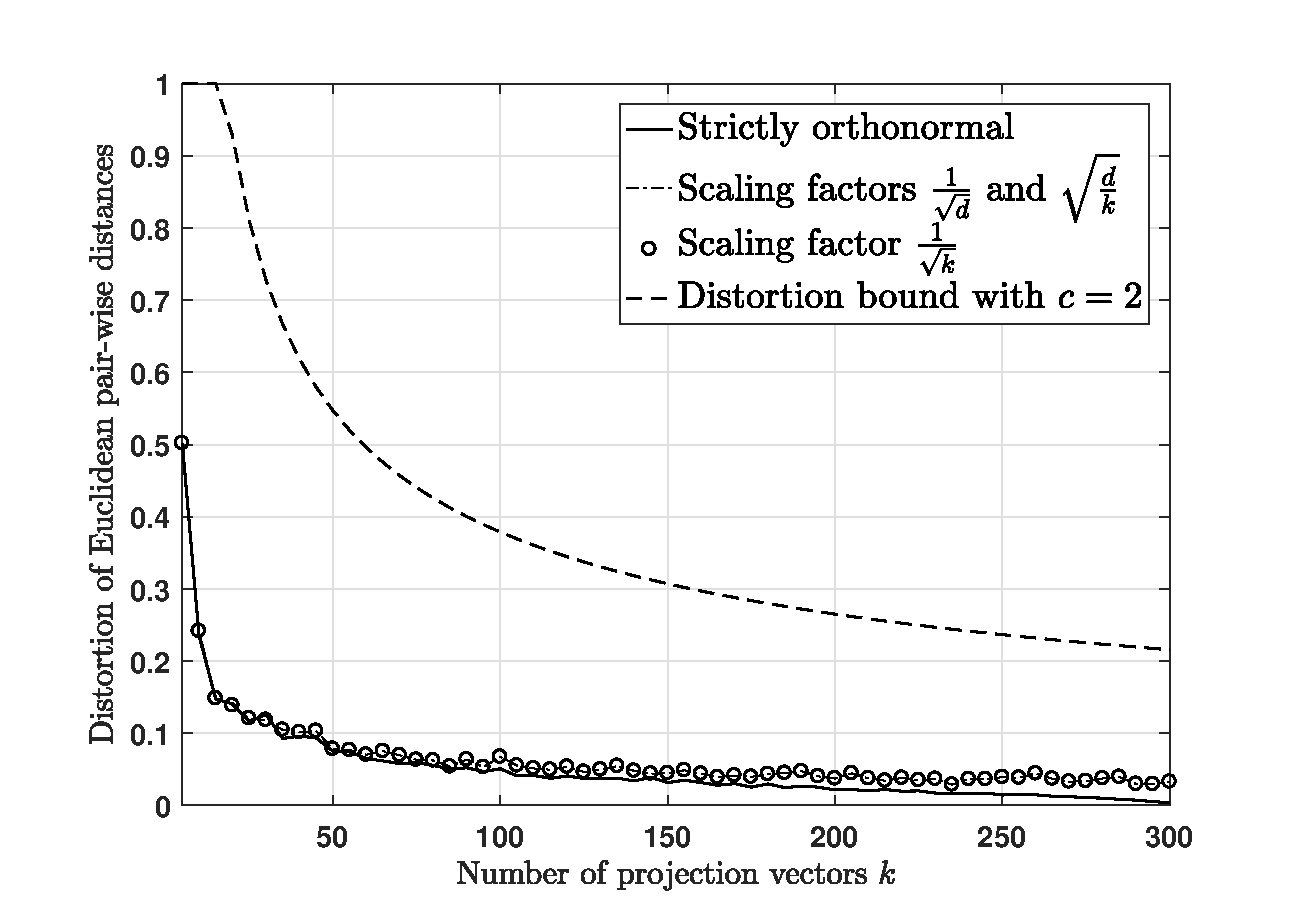
\includegraphics[scale=0.4]{rp-method/Distortion_distances}
	\vspace{-0.1cm}
	\caption{Distortion of pair-wise distances obtained by the different projection matrices and the bound on $\varepsilon$ from $k=(\frac{2}{\varepsilon^2} \ \log(n))$ \cite{venkatasubramanian2011johnson}.}
	\label{fig:distortion_distances}
\end{figure}

\newpage
However, in order to make the cheap reconstruction method as in equation \eqref{eq:reconstruction_pcareconstruction} possible, the approximately orthogonal projection vectors in $\mathbf{R}$ must be of unit length as well. To that end, figure \ref{fig:average_norms} shows that the average norm of the projection vectors with scaling factor $\frac{1}{\sqrt{k}}$ is on expectation equal to $\sqrt{\frac{d}{k}}$ instead of $1$. The norm of this projection matrix only approaches $1$ if $k$ approaches $d$. This implies that $\frac{1}{\sqrt{k}} \mathbf{R}^T \ \frac{1}{\sqrt{k}} \mathbf{R} \not\approx \mathbf{I}$ with $r \sim \mathcal{N}(0,1)$. Hence, we cannot use this short-cut in our method.

\begin{figure}[h]
	{\centering
		\vspace{-0.1cm}
		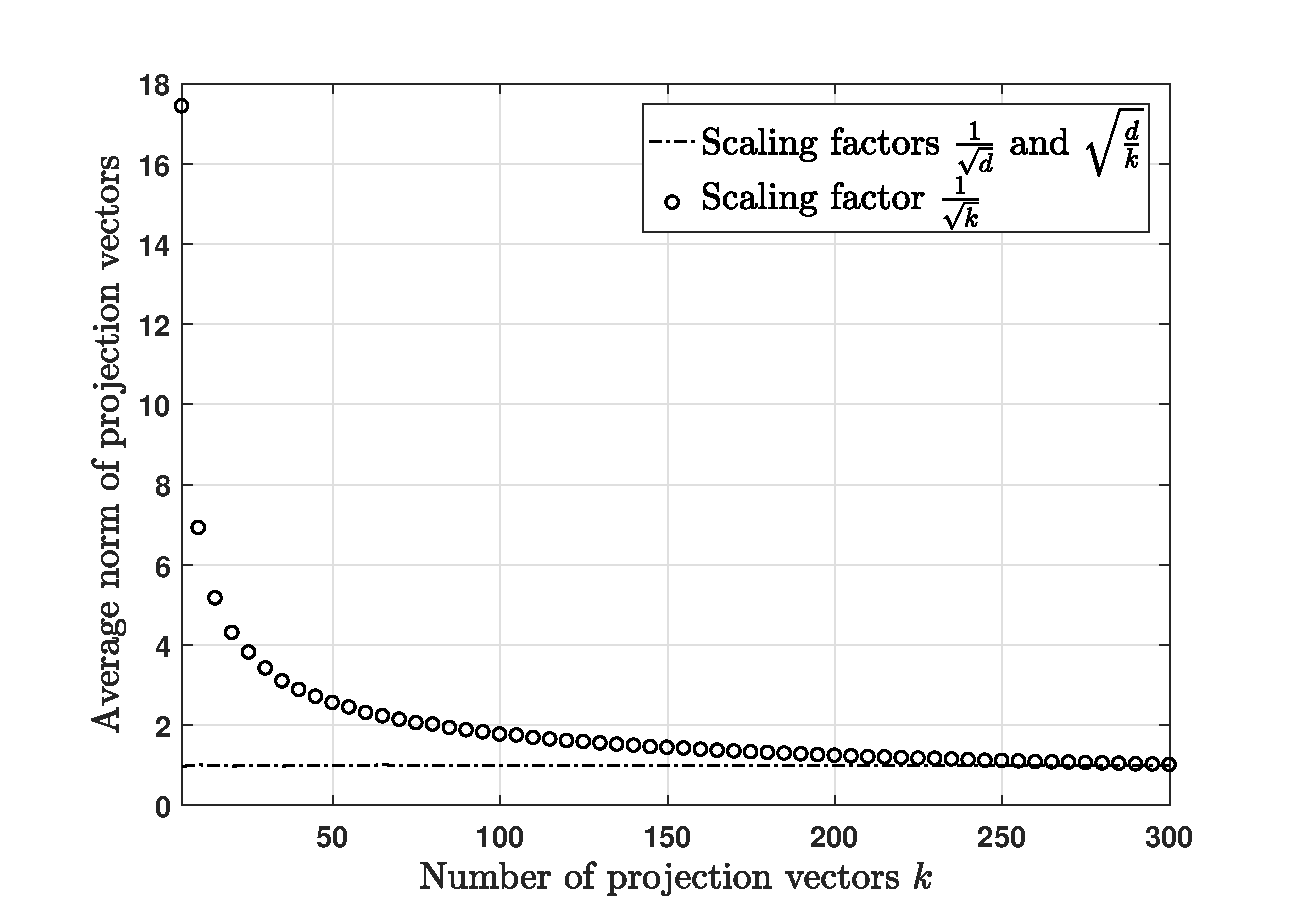
\includegraphics[scale=0.4]{rp-method/Norms_projection_vectors}
		\vspace{-0.1cm}
		\caption{Average norms of the $k$ projection vectors for $k$ ranging from $1$ to $d$.}
		\label{fig:average_norms}}
\end{figure}

Two questions remain open ended. First, how well can we reconstruct a projected vector using the cheap reconstruction method (taking the transpose $\mathbf{R}^T$ instead of the inverse $\mathbf{R}^{-1}$) from a projection matrix that is only orthonormal on expectation? Going from the following observations:

\begin{itemize}
	\itemsep0em
	\item the pair-wise Euclidean distances preserved are almost equal to the distances preserved using strictly orthogonal projection vectors as shown in figure \ref{fig:distortion_distances},
	\item the average norms of the $k$ projection vectors are very close to $1$ for $k = 1$ already, and
	\item the product $\frac{1}{\sqrt{d}}\mathbf{R}^T \ \frac{1}{\sqrt{d}}\mathbf{R}$ approximates $\mathbf{I}$ closely,
\end{itemize}

\noindent it might depend on the choice for $k$ and the original dimensionality $d$, but we have confidence it will bring the desired reconstruction results in most cases. Therefore, we will scale $\mathbf{R}$ with $r \sim \mathcal{N}(0,1)$ by the factor $\frac{1}{\sqrt{d}}$ resulting in orthonormality only on expectation, but still use the cheap reconstruction method.

The final unanswered question is whether we should care about the norm of the projection $\mathbf{x}_i'$ being scaled down with $\sqrt{\frac{k}{d}}$ on expectation? If so, at what point should we then scale it back with $\sqrt{\frac{d}{k}}$?
For separability purposes it does not make a difference if the reconstruction approaches the original data point or not as also noted in \cite{fradkin2003experiments}. Yet, for our method it is an important consideration as we actually use the difference between the reconstruction of $\mathbf{x}_i'$ as well as the original data point $\mathbf{x}_i$ to derive the outlier scores.

First, let us determine where scaling with $\sqrt{\frac{d}{k}}$ would be in place. If we would scale the projection $\mathbf{x}_i'$ of $\mathbf{x}_i$ before reconstruction, we basically reconstruct a transformed version of the original projection. For the sake of proper reconstruction, we need $\mathbf{x}_i'$ to be the original projection of $\mathbf{x}_i$. Therefore, the reconstruction $\hat{\mathbf{x}}_i$ of $\mathbf{x}_i'$ should be scaled instead, to obtain a reconstruction of which the norm ($\|\hat{\mathbf{x}_i}\|$) approximates the norm of the original data point ($\|\mathbf{x}_i\|$). To illustrate the effect of scaling the reconstruction back, figure \ref{fig:effect_backscaling} shows the difference between an example time series $\mathbf{x}_j$, its unscaled reconstruction and scaled reconstruction\footnote{The presented time series is just $1$ out of $60$ time series with random phase, amplitude, offset and noise, which causes the misalignment between the original and its reconstructions.}.

\begin{figure}[h]
	{\centering
		\vspace{-0.32cm}
		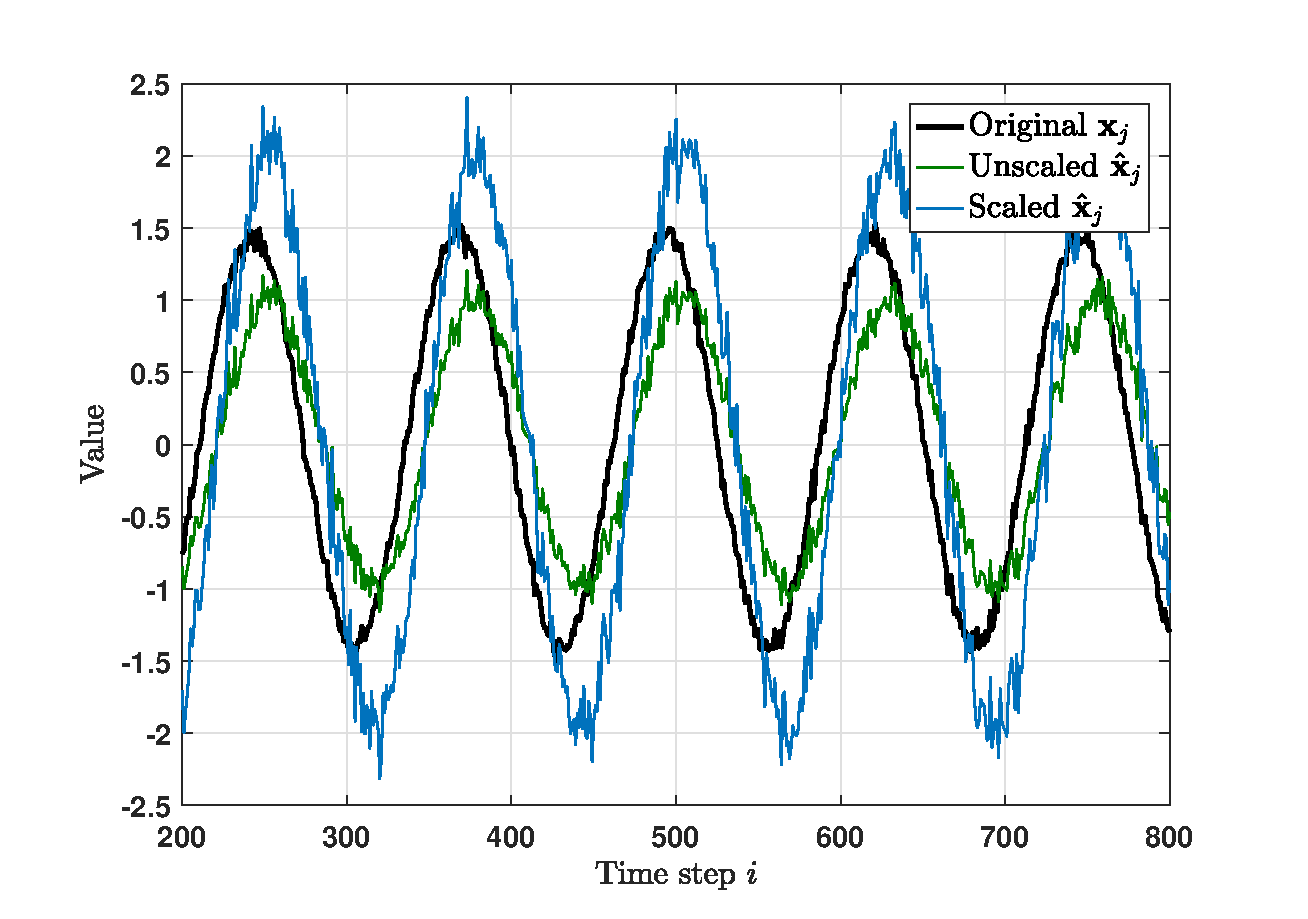
\includegraphics[scale=0.38]{rp-method/Effect_reconstruction_backscaling1}
		\vspace{-0.3cm}
		\caption{Effect of scaling the reconstruction back with $\sqrt{\frac{d}{k}}$.}
		\label{fig:effect_backscaling}}
		\vspace{-0.2cm}
\end{figure}

As can be derived from this figure, whether back-scaling improves our model for detection purposes is tightly associated with the type of outliers to be found in the data. Starting with global point outliers it seems better to use the unscaled reconstruction, as we will discriminate outliers that are far from the model by making use of the squared Euclidean distance between $\mathbf{x}_i$ and $\hat{\mathbf{x}_i}$. So, in that case we do not want our model to be closer to the original values as results from scaling the reconstructed version back with $\sqrt{\frac{d}{k}}$. This becomes clear if we consider the time series as in figure \ref{fig:effect_backscaling} and imagine a global point outlier appearing around $i=500$ (e.g. its value is around $2$ instead of $1.5$). Then the squared Euclidean distance between $\mathbf{x}_i$ and $\sqrt{\frac{d}{k}} \ \hat{\mathbf{x}}_i$ would be smaller compared to all normal data points instead of larger. The unscaled reconstruction does not suffer from this.

On the contrary, to find contextual outliers we want a model close to the original and hope it is indeed very close to the original without modelling any outliers. Considering the same example at $i=500$ but instead with its value around $1$ instead of $1.5$. We would be better off back-scaling the resulting reconstruction as we get a higher squared Euclidean distance between the model and the original point for contextual outliers.
As the success of back-scaling might depend on the data at hand, we assessed its actual influence on the outlier detection performance experimentally in chapter \ref{chap:analysis}. 

Beside the influence of the scaling factors on the outlier detection performance, our lower-dimensional representations and reconstructions are close to the mean and average range of all time series together. This implies that our method is sensitive to the mean and range of the input data. Hence, it is preferable to estimate the mean (and possibly standard deviation) of the different time series online to correct for this effect. As such online parameter estimations might not be accurate enough, we analysed the performance for standardized data such that each time series has $0$ mean and unit variance, and data of which the means and ranges are approximately equal.


\section{The proposed method}
\label{sec:method_formulation}

Altogether, the mathematical procedures to compute the projection, reconstruction and outlier score of a data point $\mathbf{x}_i$ online are quite similar to the procedures presented in chapter \ref{chap:reconstruction-detection}. That is, we obtain our projection by

\vspace{-0.2cm}
\begin{equation}\label{eq:method_projection}
\mathbf{x}_i' = \frac{1}{\sqrt{d}} \mathbf{R} \ \mathbf{x}_i
\end{equation}

\noindent where $\mathbf{R}$ is the random coefficient matrix of size $k \times d$ with entries $r \sim \mathcal{N}(0,1)$. Then the projected data point $\mathbf{x}_i'$ is easily reconstructed to its original dimensionality $d$ using

\vspace{-0.1cm}
\begin{equation}\label{eq:method_reconstruction}
\hat{\mathbf{x}}_i = \frac{1}{\sqrt{d}} \mathbf{R}^T \ \mathbf{x}_i'
\end{equation}  

\noindent where $\mathbf{R}^T$ is used instead of the inverse $\mathbf{R}^{-1}$ as we have 

\vspace{-0.1cm}
\begin{equation}\label{eq:method_orthonormality}
\frac{1}{\sqrt{d}} \mathbf{R}^T \ \frac{1}{\sqrt{d}} \mathbf{R} \approx \mathbf{I}.
\end{equation}  

Finally, as mentioned in the previous section, it depends on the data (and outliers) and the quality of the projections and reconstructions if back-scaling results in a more accurate model close to the original data point. For the sake of completeness, if one wants a reconstruction closer to the original data point, we need to scale the reconstruction by

\vspace{-0.1cm}
\begin{equation}\label{eq:method_scaledreconstruction}
\hat{\mathbf{x}}_i \gets \sqrt{\frac{d}{k}} \ \hat{\mathbf{x}}_i
\end{equation} 

\noindent The outlier score $O_i$ is computed similarly as in equation \eqref{eq:reconstruction_score}. Each outlier score should then be converted to an actual binary label (e.g. $0$ for normal data points and $1$ for outliers). To do so, a threshold $\theta$ should be set such that if $O_i \leq \theta$ the corresponding data point is labelled as normal else as an outlier. Eventually, we want $\theta$ to minimize the error between all the predicted and actual labels\footnote{Misclassified outliers might be more costly than misclassified normal data points or vice versa, therefore $\theta$ actually optimizes the weighted balance between these two. This is explained in chapter \ref{chap:analysis}.}. Algorithm \ref{alg:analysis_algorithm} presents the final algorithm we propose.

\vspace{-0.2cm}
\begin{algorithm}[H]
	\vspace{-0.1cm}
	\caption{\quad \textbf{RP}}
	\label{alg:analysis_algorithm}
	\begin{flushleft}
		\vspace{-0.2cm}
		\textbf{Input} data point $\mathbf{x}_i$ of size $d \times 1$\\	
		\textbf{Input} number of projection vectors $k$	
		\vspace{-0.1cm}
	\end{flushleft}
	\begin{algorithmic}[1]
		\vspace{-0.2cm}
		\IF{$i=1$}
			\STATE Generate ${\mathbf R}$ of size $k \times d$ with entries $r \sim \mathcal{N}(0,1)$
		\ENDIF
			\STATE Project $\mathbf{x}_i$ on $\mathbf{R}$ by ${\mathbf x}_i' = \frac{1}{\sqrt{d}} {\mathbf R} \ {\mathbf x}_i$ 
			\STATE Reconstruct ${\mathbf x}_i'$ to $\hat{{\mathbf x}}_i = \frac{1}{\sqrt{d}} {\mathbf R}^T \ {\mathbf x}_i'$
		\IF{approximate norm preservation is desired}
			\STATE Scale reconstruction back $\hat{\mathbf{x}}_i = \sqrt{\frac{d}{k}} \hat{\mathbf{x}}_i$
		\ENDIF
		\STATE $O_i = \|{\mathbf x}_i - \hat{{\mathbf x}}_i\|^2$
	\end{algorithmic}
	\begin{flushleft}
		\vspace{-0.3cm}
		\flushleft\textbf{Output} outlier score $O_i$
	\end{flushleft}
\end{algorithm}
\vspace{-0.2cm}

To deploy the RP method for outlier detection in multivariate time series, we just need to generate $\mathbf{R}$ once at the start of the stream $\mathbf{X}$. From there, we only need $2$ matrix-vector multiplications resulting in a runtime of $\mathcal{O}(kd)$ per data point as well. Though it seems close to $\mathcal{O}(k^2d)$, it depends quadratically on $k$ and the constant hidden in this upper bound associated with SPIRIT is higher. If we consider, for instance, algorithms \ref{alg:spirit} and \ref{alg:trackw} it becomes clear that SPIRIT conducts more matrix-vector multiplications to update the principal coefficient matrix $\mathbf{W}$ than needed with the RP method. In chapter \ref{chap:analysis} we experimentally explored the behaviour of the runtime of SPIRIT for varying values of $d$ and $k$.


\chapter{Analysis}
\label{chap:analysis}

In this chapter we analyse the performance of the RP method for online outlier detection in multivariate time series. We explain the analysis setup in section \ref{sec:analysis_methodology}, after which we provide more insight in the inner working of the RP method in section \ref{sec:analysis_innerworking}. In section \ref{sec:analysis_bird} we analyse the method under varying parameter settings. We also investigate the influence of back-scaling for different types of outliers. In section \ref{sec:analysis_contextual} we explain how we use the method in a slightly different manner, and analyse its performance accordingly. Section \ref{sec:analysis_worm} presents the performances under fixed parameter settings to assess both uses of the method in online mode. Section \ref{sec:analysis_concluding} concludes with a summary of the key findings.


\section{Analysis setup}
\label{sec:analysis_methodology}

In this thesis, we focus on the task of online unsupervised outlier detection in multivariate time series. We discussed the most important challenges imposed by this task in table \ref{tab:intro_characteristics}. The central objective of this analysis is to assess the applicability of the proposed method given these challenges. To that end, we translated them into a set of evaluation criteria which we, in turn, linked to measurable performance metrics to guide this analysis and the real-world experiments following in chapter \ref{chap:experiments}. This translation is presented in table \ref{tab:analysis_evaluation}. 

In the remainder of this section we explain the synthetic data and performance metrics used for the analysis. Obviously, a method can be optimized such that it evaluates very well given one criterion, but performs horrible given another. Therefore, we make up a qualitative comparative judgement on the criteria all together in section \ref{sec:analysis_concluding}.

\begin{table}[h]
	\centering
	\hspace{-0.5cm}
	\vspace{-0.25cm}
	\caption{Evaluation criteria for this analysis and the real-world experiments in chapter \ref{chap:experiments}.}
	\label{tab:analysis_evaluation}
	\small
	\begin{tabular}{l l l}
		\toprule
		\textbf{Challenge} & \textbf{Evaluation criterion} & \textbf{Performance metric}\\ \midrule
		The algorithm must assign label $O_i$ 		& 	\multirow{2}{*}{Time needed to process data points} &  \multirow{2}{*}{Runtime performance.}	\\
		to data point $\mathbf{x}_i$ before receiving $\mathbf{x}_{i+1}$	& 	&		 \\[0.15cm]
		The algorithm should only need a limited	& \multirow{2}{*}{Dependence on history of stream} & Number of preceding  \\
		history of the data to infer its model & & data points $p$ needed. \\[0.15cm]
		
		The algorithm should run unsupervised & Amount of prior information needed & Number of parameters.\\[0.15cm]
		The detection performance should not be & Sensitivity of detection	performance to & \multirow{2}{*}{Detection performance.} \\
		too sensitive to the (fixed) parameters & parameters &  \\ \midrule
		
		The analyst should have an idea 	& Generalizability of performances to  & Stability of detection and \\
		of the data and outliers at hand 	& (un)standardized and different data sets & runtime performance. \\[0.15cm]
		The algorithm should be able to detect & Generalizability of performances to	& Stability of detection  \\
		global and contextual outliers & different outlier types 			& performance. \\ \midrule
		
		The algorithm should be able to find 	& Influence of $d$ and $n$ on detection		& Scalability of detection \\
		outliers in high-dimensional data 		& performance 			& performance. \\[0.15cm]
		Algorithms should scale in computational &	\multirow{2}{*}{Influence of $d$ on	runtime performance} & Scalability of runtime \\
		complexity with increasing $d$ 	& 		& performance.\\ \bottomrule		
	\end{tabular}
\vspace{-0.3cm}
\end{table}

\subsection{Data}

As limited qualitative labelled data sets are available that fully meet the conditions of the considered problem context, we turned to artificial data sets for the in-depth analysis of our method. An assessment of the RP method on real-world data follows in chapter \ref{chap:experiments}.
We kept the structure in our data simple by generating just $60$ time series of length $981$ from sinusoidal functions each with a different phase (sine or cosine), additional random misalignment ($\varphi$), amplitude ($A$) and offset ($C$). We also added a time-depending noise term $N_t$ to avoid smooth time series. The specific function underlying each time series in our artificial data set is as follows

\begin{equation}\label{eq:analysis_data}
 \mathbf{x}(t) = 
	\begin{cases} 
		A \sin(t + \varphi) + C + N_t	& \text{with probability } \frac{1}{2} \\[0.5em]
		A \cos(t + \varphi) + C + N_t   & \text{with probability } \frac{1}{2},
	\end{cases}
\end{equation}
\vspace{0.2cm}

\noindent with $t$ from $1$ to $50$ with an interval of $0.05$, $A \sim \mathcal{U}(1,3)$, $\varphi \sim \mathcal{N}(0,1)$, $C \sim \mathcal{U}(0,1)$ and $N_t \sim \mathcal{N}(0,0.05)$. From this point onwards, we refer to each time step $t$ with integer values $i$ from $1$ to $981$. Like in many real-world applications, the distinct time series have a different range and not necessarily $0$ mean. Online procedures are available to standardize the time series to $0$ mean with unit variance, of which a common method is discussed in section \ref{sec:analysis_contextual}. In practice such online methods do not perfectly standardize the data over the entire stream. Therefore, to analyse the random projection method in a realistic setting we introduced the offset term $C$. The analysis results with standardized data are presented and discussed in the appendix \ref{app:analysis}.

We created $3$ distinct copies of the resulting $60 \times 981$ clean data set and injected each data set with either global point outliers, contextual point outliers or contextual collective outliers. First, we randomly sampled $6$ distinct subsets of $12$ (out of $60$) time series, where we injected $1$ of the $3$ outlier types in each pair of $2$ subsets. The global point outliers were created by multiplying $6$ random sequences of $3$ data points with an arbitrary large factor of $1.5$, i.e. \{$\tilde{\mathbf{x}}_{i,j} = 1.5 \ \mathbf{x}_{i,j} : i=1,2,3$\} with $j$ the time series from the respective subset. The contextual point outliers were obtained by multiplying $6$ random sequences of $3$ data points with a small enough factor of $0.1$, i.e. \{$\tilde{\mathbf{x}}_{i,j} = 0.1 \ \mathbf{x}_{i,j} : i=1,2,3$\}. The collective outliers were obtained by replacing $4$ random sequences of $15$ data points with the values at the first time step of that time series $j$, i.e. \{$\tilde{\mathbf{x}}_{i,j} = \mathbf{x}_{1,j} : i=1,2,...,15 $\}. The outlier characteristics are summarized in table \ref{tab:analysis_outliers}.

\begin{table}[h]
	\centering
	\caption{Summary of the outliers in the synthetic time series.}
	\label{tab:analysis_outliers}
	\begin{tabular}{l c c c  }
		\toprule	
		\multirow{2}{*}{\textbf{Outlier type}} & \textbf{$\#$ responsive} & \textbf{$\#$ outlying} & \textbf{Feature value} \\
		&  \textbf{time series} & \textbf{data points} & \textbf{of time series $j$} \\
		\midrule
		Global point			& $2$ subsets of $12$	& $6 \cdot 3 = 18$  & $\tilde{\mathbf{x}}_{i,j} = 1.5 \  \mathbf{x}_{i,j}$ 	\\
		Contextual point		& $2$ subsets of $12$ 	& $6 \cdot 3 = 18$  & $\tilde{\mathbf{x}}_{i,j} = 0.1 \  \mathbf{x}_{i,j}$	\\
		Contextual collective	& $2$ subsets of $12$	& $4 \cdot 15 = 45$  & $\tilde{\mathbf{x}}_{i,j} = \mathbf{x}_{1,j}$	\\
		\bottomrule
	\end{tabular}
\end{table}

Parts of $3$ of the $60$ resulting time series with the different outlier types are shown in figures \ref{fig:analysis_point} to \ref{fig:analysis_collective}. Clearly, we have correlating and stationary time series what might be different in real-world applications. In chapter \ref{chap:experiments} we assess and compare the performances on (more) realistic data.

\begin{figure}[h]
	\begin{minipage}{0.333\textwidth}
		\centering
		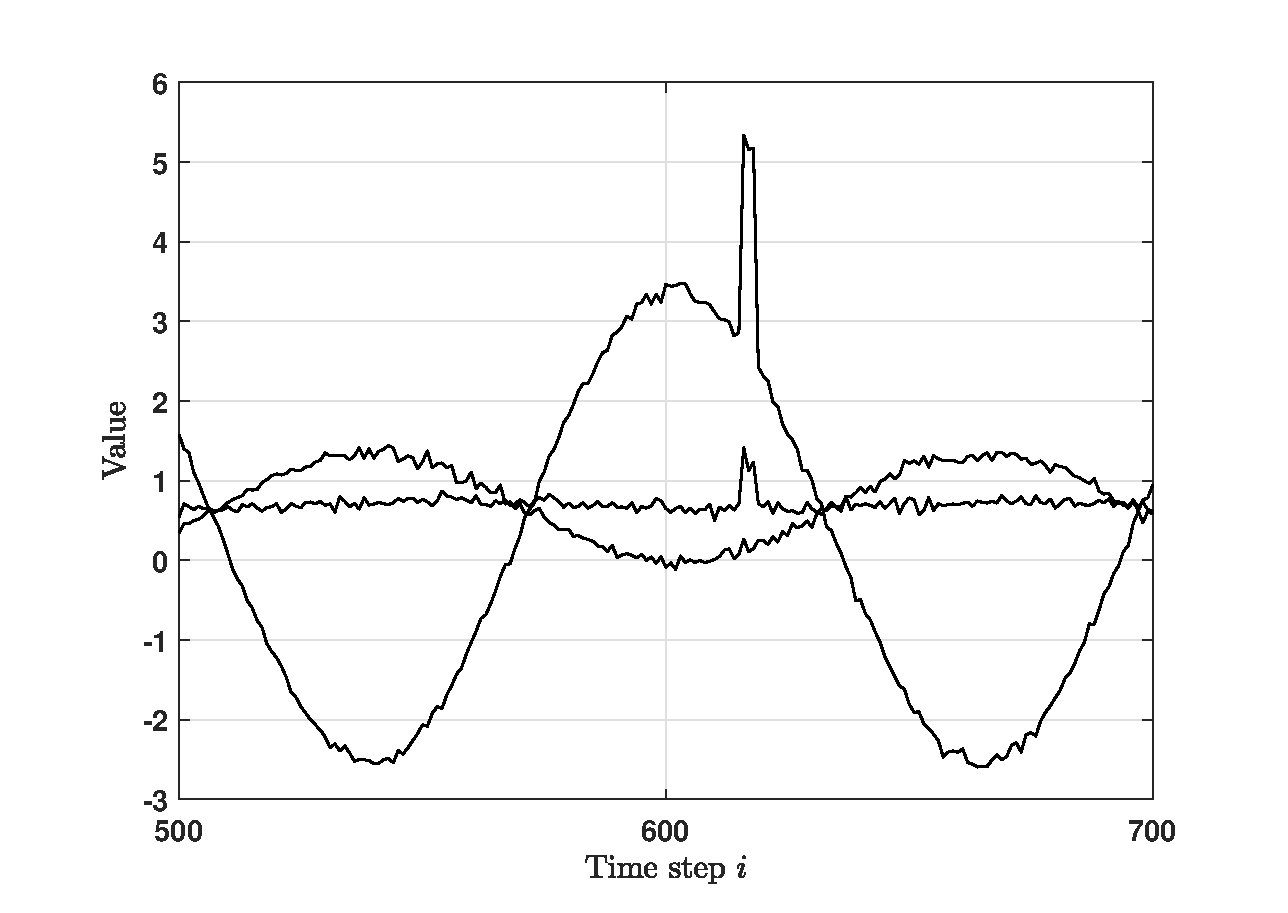
\includegraphics[scale=0.27]{analysis/Example_timeseries_point_frac}
		\caption{Global point}
		\label{fig:analysis_point}
	\end{minipage}
	\begin{minipage}{0.333\textwidth}
		\centering
		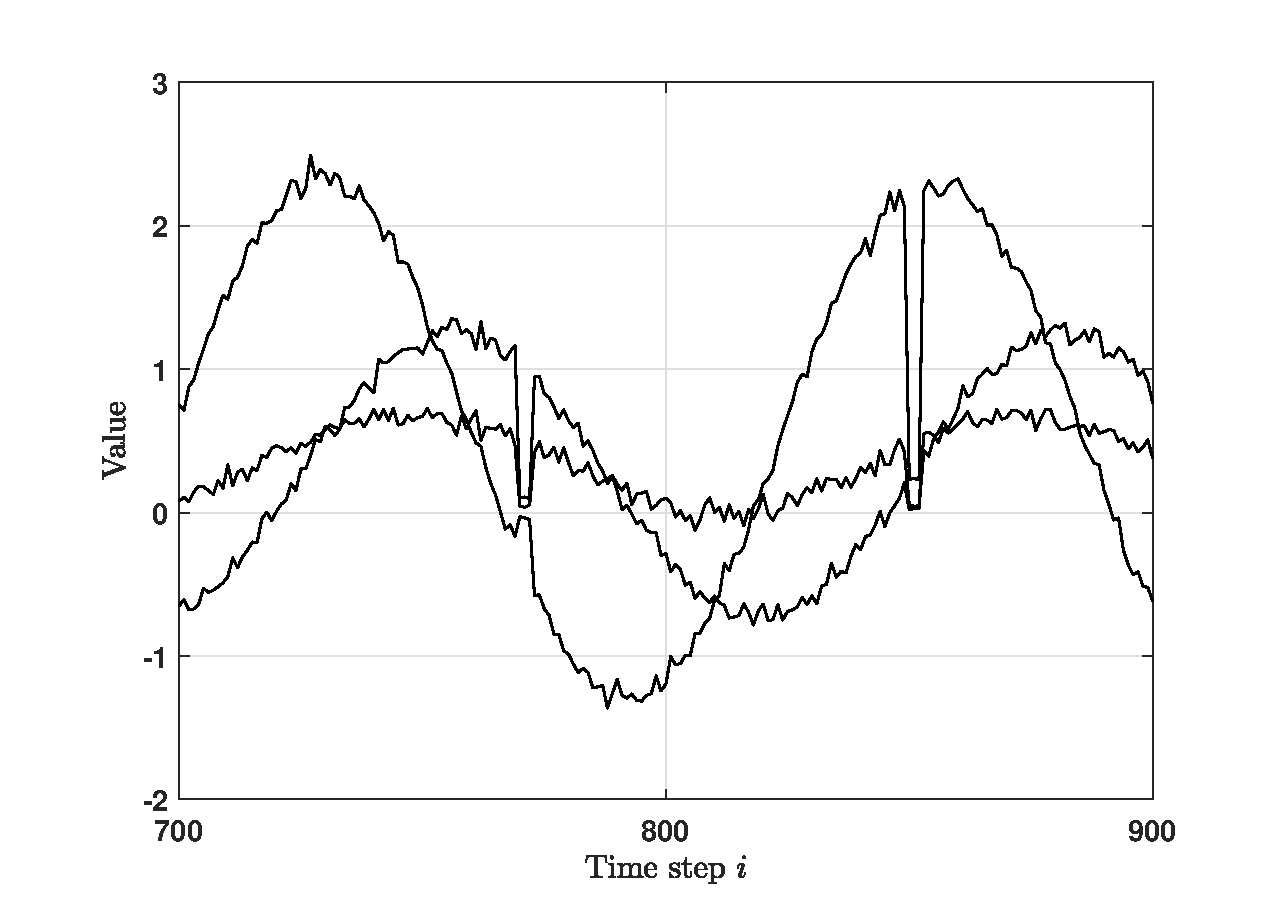
\includegraphics[scale=0.27]{analysis/Example_timeseries_contextual_frac}
		\caption{Contextual point}
		\label{fig:analysis_contextual}
	\end{minipage}
	\begin{minipage}{0.333\textwidth}
		\centering
		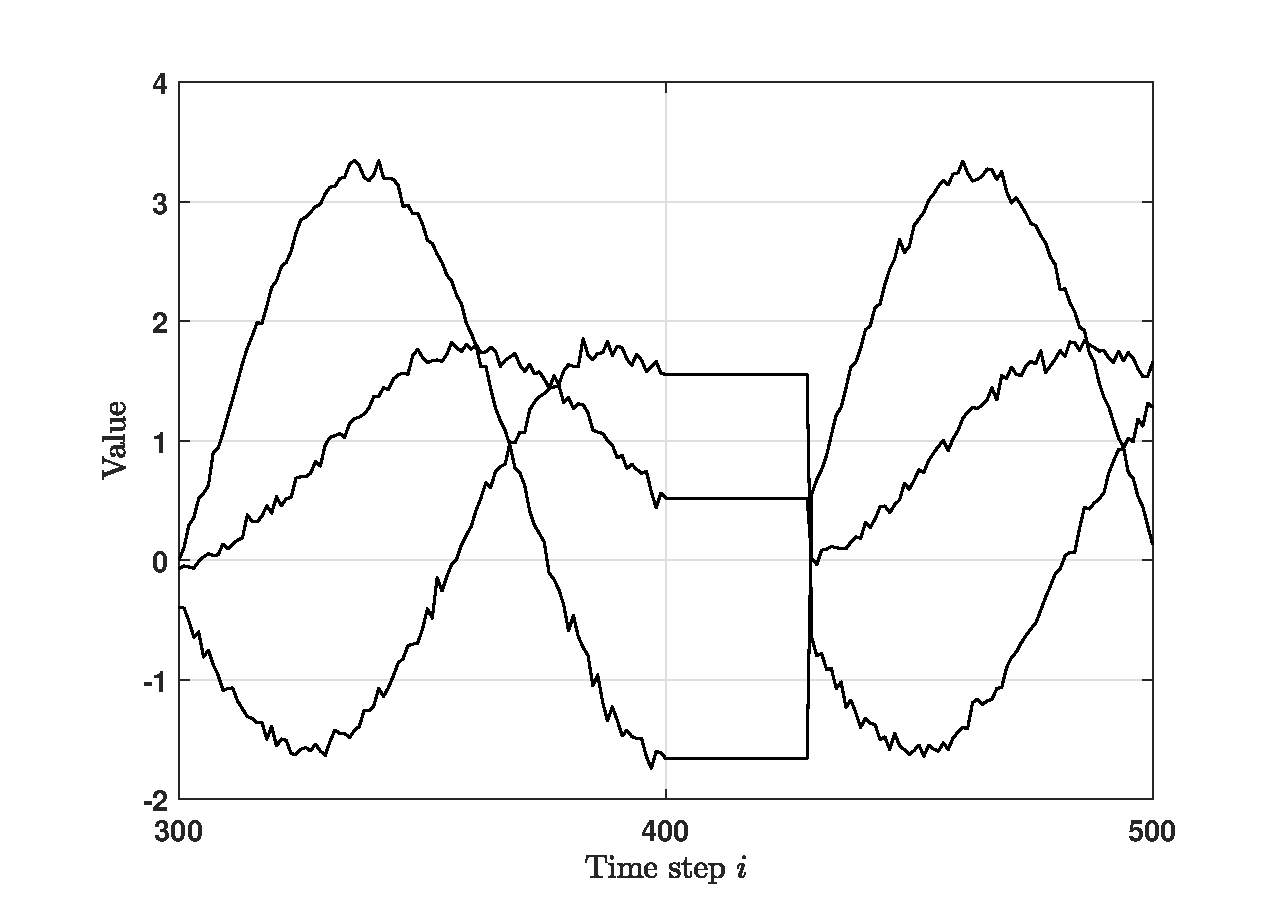
\includegraphics[scale=0.27]{analysis/Example_timeseries_collective_frac}
		\caption{Contextual collective}
		\label{fig:analysis_collective}
	\end{minipage}
\end{figure}

For outlier detection in multivariate time series a sliding window is often implemented to not only look at a single data point $\mathbf{x}_i$ to derive its outlier score, but look at $\mathbf{x}_i$ given its history of length $p$. This way we might be better in detecting interruptions of the temporal continuity exhibited in stream $\mathbf{X}$. Applying a sliding window, therefore, particularly benefits commonly used methods to detect contextual outliers. A sliding window can be established by just concatenating each $\mathbf{x}_i \in \mathbb{R}^d$ with its $p$ previous values $\mathbf{x}_{i-1},\mathbf{x}_{i-2},...,\mathbf{x}_{i-p}$ resulting in $\mathbf{x}_i \in \mathbb{R}^{d \cdot p}$.
Technically this translates to classifying sequences of $p$ data points instead of single data points, but as the window slides only 1 step further we can interpret this as classifying $\mathbf{x}_i$ given its previous $p$ values. Each window $\mathbf{x}_i \in \mathbb{R}^{d \cdot p}$ is labelled as outlier if at least one of the data points $\mathbf{x}_i,...\mathbf{x}_{i-p} \in \mathbb{R}^d$ is an outlier. We end up with $(n − p + 1)$ data points in each data set. 

For this analysis we considered window lengths of $1, 5, 10$ and $15$, where $p=1$ reflects the original data set where no sliding window is implemented and we classify the single data points. In short, we obtained data sets of sizes as in table \ref{tab:analysis_datasets}.

\begin{table}[h]
	\centering
	\caption{Dimensionality of data sets with sliding windows.}
	\label{tab:analysis_datasets}
	\begin{tabular}{ c c c }
		\toprule	
		\textbf{Original} & \multirow{2}{*}{\textbf{Window length $p$}}  & \textbf{Resulting} \\
		\textbf{dimensionality} & & \textbf{dimensionality} \\
		\midrule
		\multirow{4}{*}{$60 \times 981$} & $1$ 	& $60 \times 981 $ 	\\
									 	 & $5$ 	& $300 \times 977$	\\
										 & $10$	& $600 \times 972$ 	\\
										 & $15$	& $900 \times 967$ 	\\
		\bottomrule
	\end{tabular}
\end{table}


\subsection{Performance metrics}

\subsubsection{\textit{Runtime performance}}

Even though we already provided the upper bounds for the runtime complexity of the methods we also investigated their runtime in practice. This enables us to investigate the runtime behaviour of the algorithms for different settings of the parameters. We do not interpret the actual time that it takes to run the algorithms as that depends on machine configurations and is not in our interest, we merely use it as a mean to see how methods compare to each other. For all experiments we measured the time it takes before a method has computed the outlier scores for all $\mathbf{x}_i \in \mathbf{X}$. We used built-in functions $\texttt{tic}$ and $\texttt{toc}$ of Matlab which measure the wall-clock runtime time, i.e. the actual time it takes to execute all operations between commands $\texttt{tic}$ and $\texttt{toc}$. 

\subsubsection{\textit{Number of parameters and preceding data points needed}}
The amount of prior information incorporated in a method is preferred to be minimal in order to make it generalize well to an unseen (and dynamically changing) data stream. The more parameters a method has, the more prior information is needed or guesses have to be made by the analyst to set them properly. Hence, the number of parameters needed to deploy a method seemed to be a good indicator of the prior information consumed by it. 
Altogether, this could make a method suffer from poor generalizability. The number of parameters might however be a bit more nuanced than just being a number. If the analyst has a good idea about a suitable parameter setting before running the system, the number of parameters might not be as critical after all. The impact of this performance metric also strongly coheres with the sensitivity of the detection performance to the parameters.

The number of historic data points needed to process the current data point, if needed at all, by an online method is also considered an important metric. Beside the possible effect on the runtime, it also requires memory storage which is intended to be minimized. As already explained, we created data sets to imitate a sliding window in a data stream. The length $p$ of such a sliding window directly reflects the number of historic data points used. Methods that need a large value for $p$ are less in favour than methods that only need little or no history of a data stream.

\subsubsection{\textit{Detection performance}}

To assess outlier detection methods it is important to realize we are dealing with imbalanced classes. That is, the class of outliers is often much smaller than the class of normal data points. In class-imbalanced situations just taking the ratio of correctly classified data points out of the entire stream does not reflect the detection performance of the method if we want to detect outliers. For example, if we have a classification problem with $95$ normal data points and $5$ outliers, classifying all outliers as normal data points already results in an accuracy of $95\%$. But in that case, we ignore all the outliers we actually wanted to detect with the outlier detection method. 

Instead of simply counting each misclassified data point regardless of whether it is an outlier or normal data point, we separate these counts and refer to outliers as `positives' and the normal data points as `negatives'. Then, a correctly classified outlier is a true positive (TP) and a normal data point classified as an outlier a false positive (FP). Correctly classified normal data points are referred to as true negatives (TN) and outliers classified as being normal as false negatives (FN). 
Eventually we want to find a balance between the number of TP's, FP's, TN's and FN's. For outlier detection methods important metrics that reflect this balance are the True Positive Rate (TPR) and False Positive Rate (FPR) as in equation \eqref{eq:analysis_tprfpr}.

\begin{equation}\label{eq:analysis_tprfpr}
	\text{TPR} = \frac{\text{TP}}{\text{P}} \ , \quad \text{FPR} = \frac{\text{FP}}{\text{N}}
\end{equation}

The TPR reflects the fraction of true detections, i.e. the correctly labelled outliers, over the full number of outliers present in the data. The FPR reflects the fraction of false detections, i.e. the incorrectly labelled normal data points, over the full number of normal data points in the data. The trade-off between these two metrics is found interesting for outlier detection \cite{zimek2012survey}. As we do not implement a threshold method, our method does not output a final label $0$ for normal data points and $1$ for outliers. To that end, we use the Receiver Operating Characteristic (ROC) to inspect the possible balances between the TPR and FPR. The ROC curve computes this balance for all possible thresholds given the outlier scores assigned to the data points. An example of an ROC curve is given in figure \ref{analysis:roc_example}. Each point on this curve represents a possible balance between the TPR and FPR associated with a fixed value for the threshold $\theta$.

\begin{figure}[h]
	\centering
	\vspace{-0.15cm}
	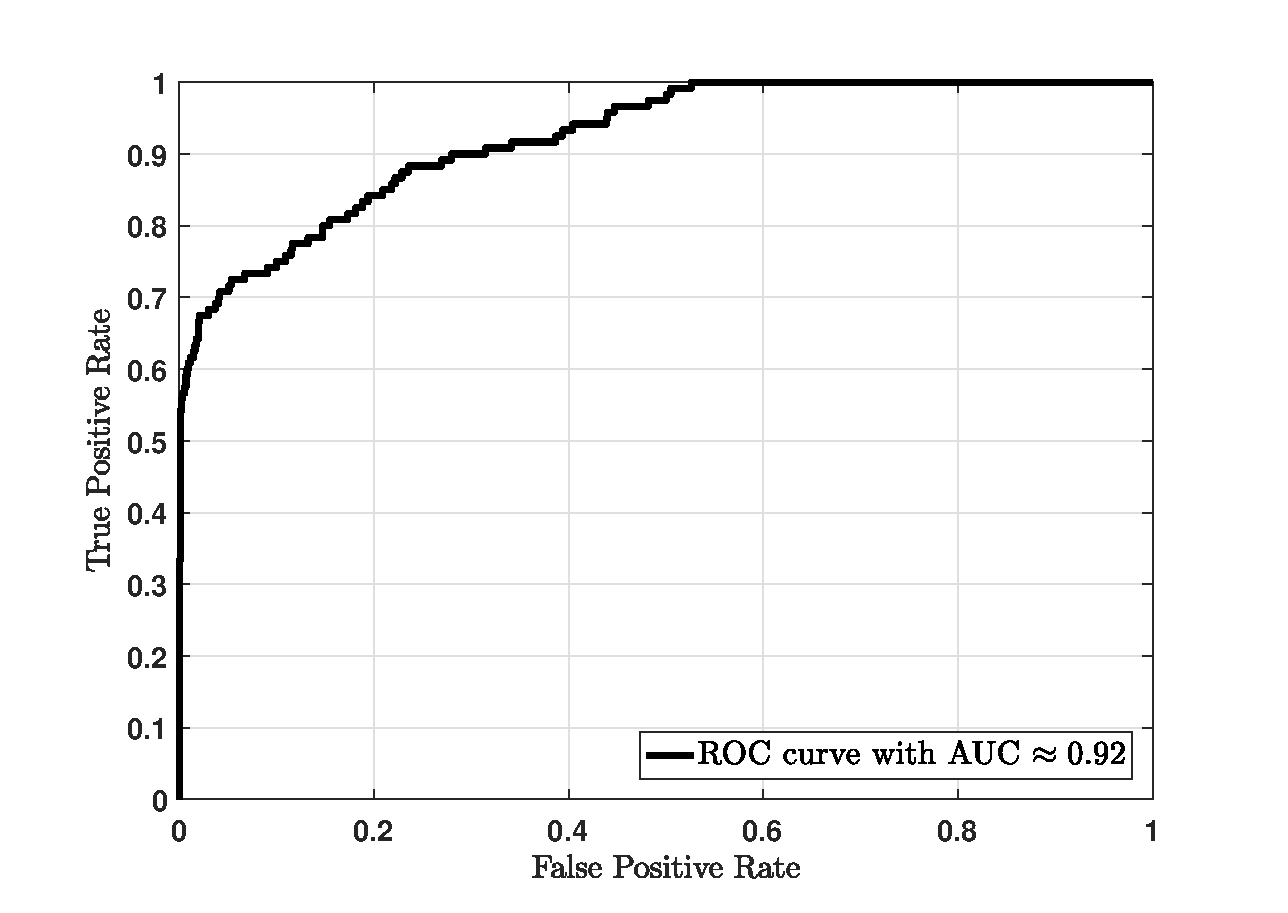
\includegraphics[scale=0.38]{analysis/Example_ROC}
	\caption{Example Receiver Operating Characteristic (ROC) curve.}
	\label{analysis:roc_example}
\end{figure}

Ideally we would have a TPR of $1$ against an FPR of $0$, so we favour methods that result in curves that are closest to the upper left corner. However, for different applications, a different balance between these two criteria is desired. As we do not focus on a particular application and so we do not have a specific desire for this balance, we prefer a neutral comparison metric to compare different ROC curves. The Area Under this (ROC) Curve (AUC) provides us the means to do this and also makes numeric comparison easier. The AUC is said to reflect the probability of a randomly selected pair of data points, of which each belongs to the opposite class, will be correctly classified in the sense that the outlier is assigned with a higher probability of being an outlier and vice versa \cite{hanley1982meaning}. Therefore, the AUC also enables interpretation of the ROC curves. 

The disadvantage of evaluating the detection performance of our online methods with the ROC and corresponding AUC, is that each operating point is based on the same threshold for all outlier scores and thus data points. This possibly yields a biased reflection of the actual detection performance \cite{mchugh2000testing}. That is, the actual threshold is not learned from all outlier scores on forehand and would probably be adaptive in our problem context. A commonly used threshold is the $3\sigma$-rule which assumes outliers to have scores of $3$ standard deviations from the mean outlier score \cite{zimek2012survey}. 


\section{The inner working of the RP method}
\label{sec:analysis_innerworking}

In chapter \ref{chap:rp-method} we presented two reconstructions (with and without back-scaling factor $\sqrt{\frac{d}{k}}$), and the corresponding original time series. This example was chosen to illustrate the effect of back-scaling, but only reflects the inner working of our method to a limited extent. Before we continue with analysing the performance of the proposed method, we first present a more thorough explanation of what it actually does.
We do so for the original time series with means close to $0$, and their standardized versions which have exactly $0$ mean and unit variance. Furthermore, we deployed the method without back-scaling, as we have taken the data set with global point outliers for this example.

Figures \ref{fig:analysis_innerworking_original} to \ref{fig:analysis_innerworking_outlierscores} illustrate the entire procedure of the RP method from original time series to the derivation of outlier scores. All figures at the left correspond to the unstandardized time series, where the right-hand side corresponds to the standardized time series. Starting with the original input in figure \ref{fig:analysis_innerworking_original}, note that instead of all $60$ time series we only show a subset of $12$ which were injected with global point outliers to avoid occlusion. Yet the RP method was deployed with all $60$ time series of length $981$ as input.
 
\begin{figure}[h]
	\centering
	\vspace{-0.12cm}
	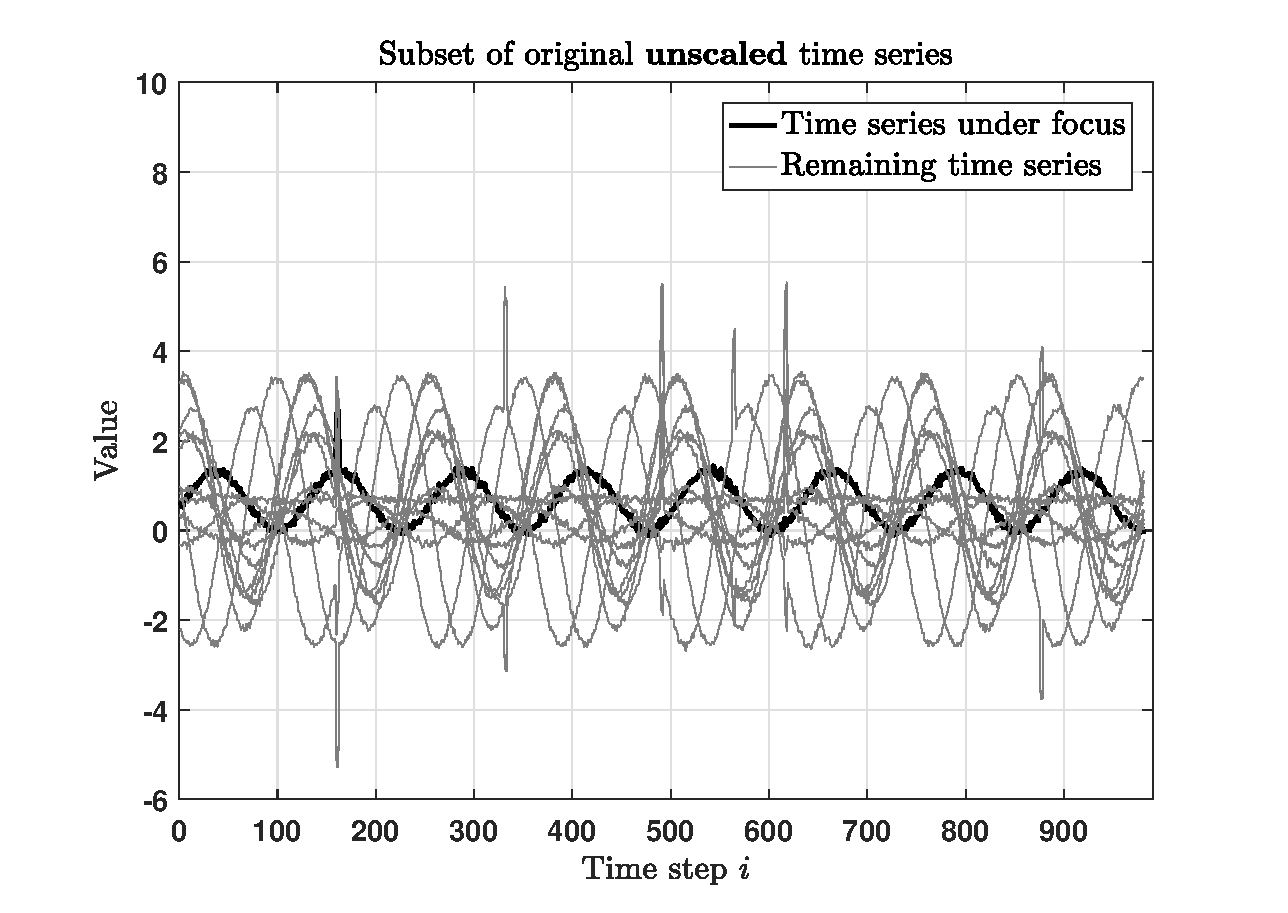
\includegraphics[scale=0.345]{analysis/Analysis_unscaled_original}
	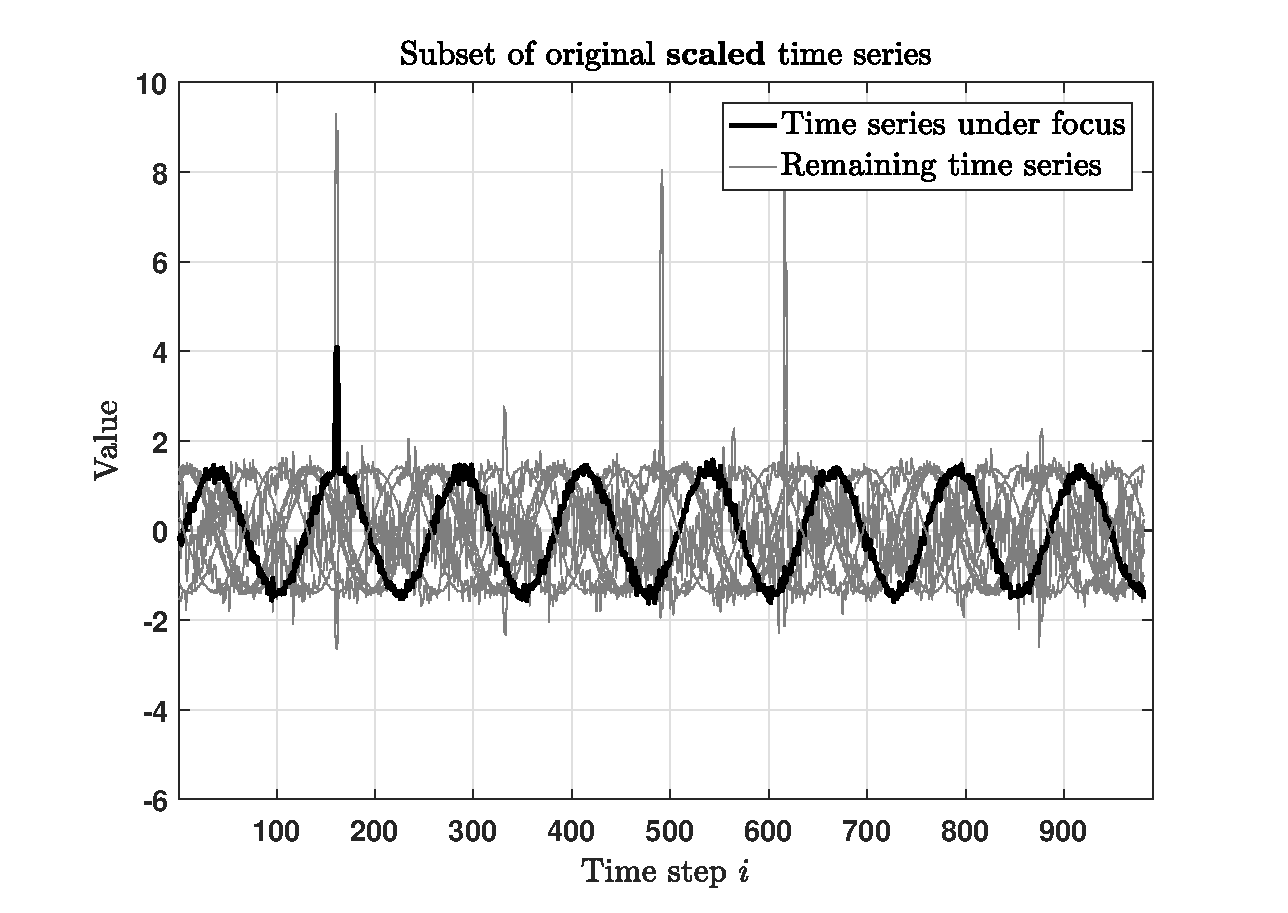
\includegraphics[scale=0.345]{analysis/Analysis_scaled_original}
	\vspace{-0.12cm}
	\caption{Original unstandardized (left) and standardized (right) subset of time series.}
	\label{fig:analysis_innerworking_original}
	\vspace{-0.1cm}
\end{figure}

Each of these $981$ $60$-dimensional data points are then projected one by one onto a $k$-dimensional projection basis, where for visualization purposes we have set $k$ to $1$ for this example. Figure \ref{fig:analysis_innerworking_projection} shows the resulting $1$D projection of the $60$D time series. 

\begin{figure}[h]
	\centering
	\vspace{-0.12cm}
	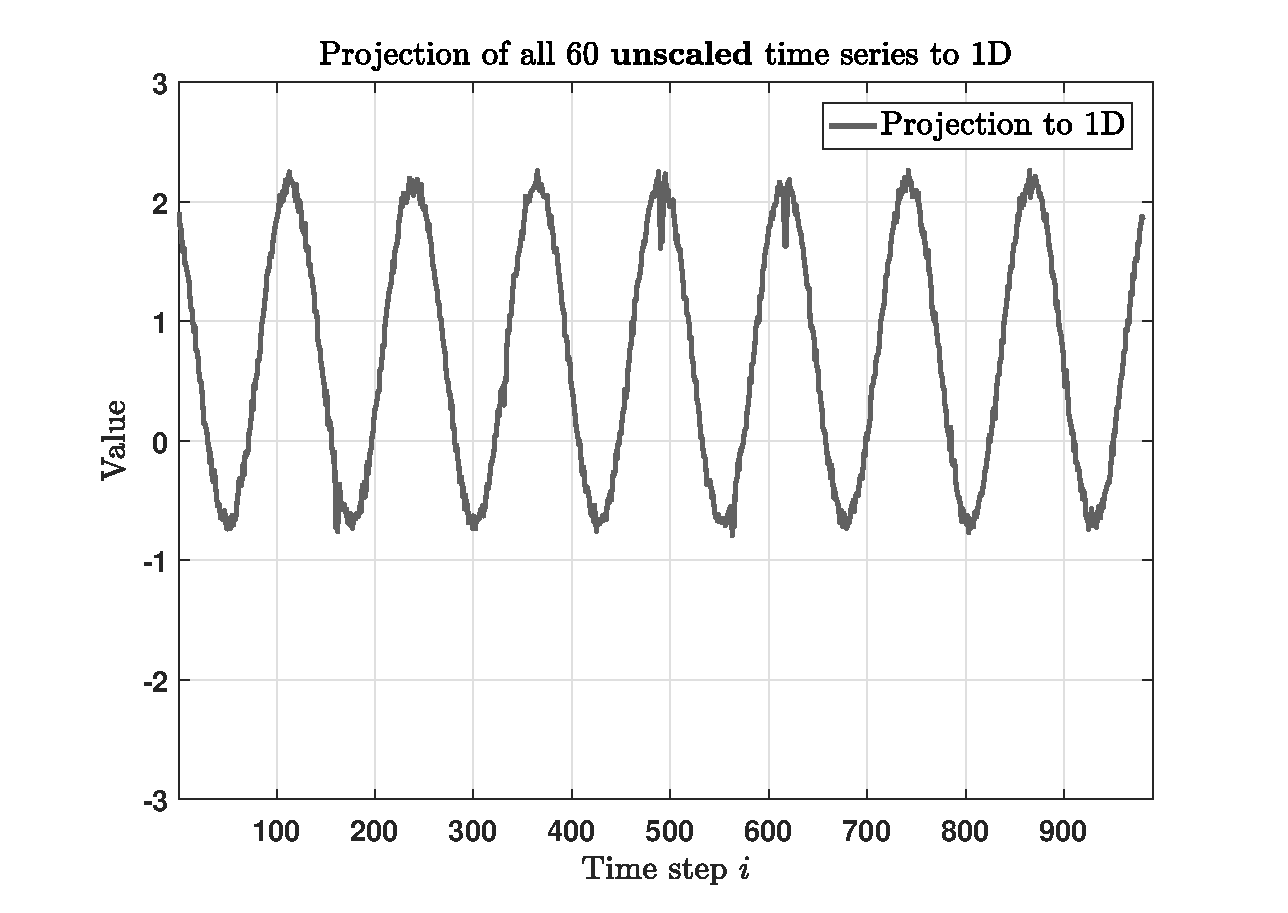
\includegraphics[scale=0.345]{analysis/Analysis_unscaled_projection}
	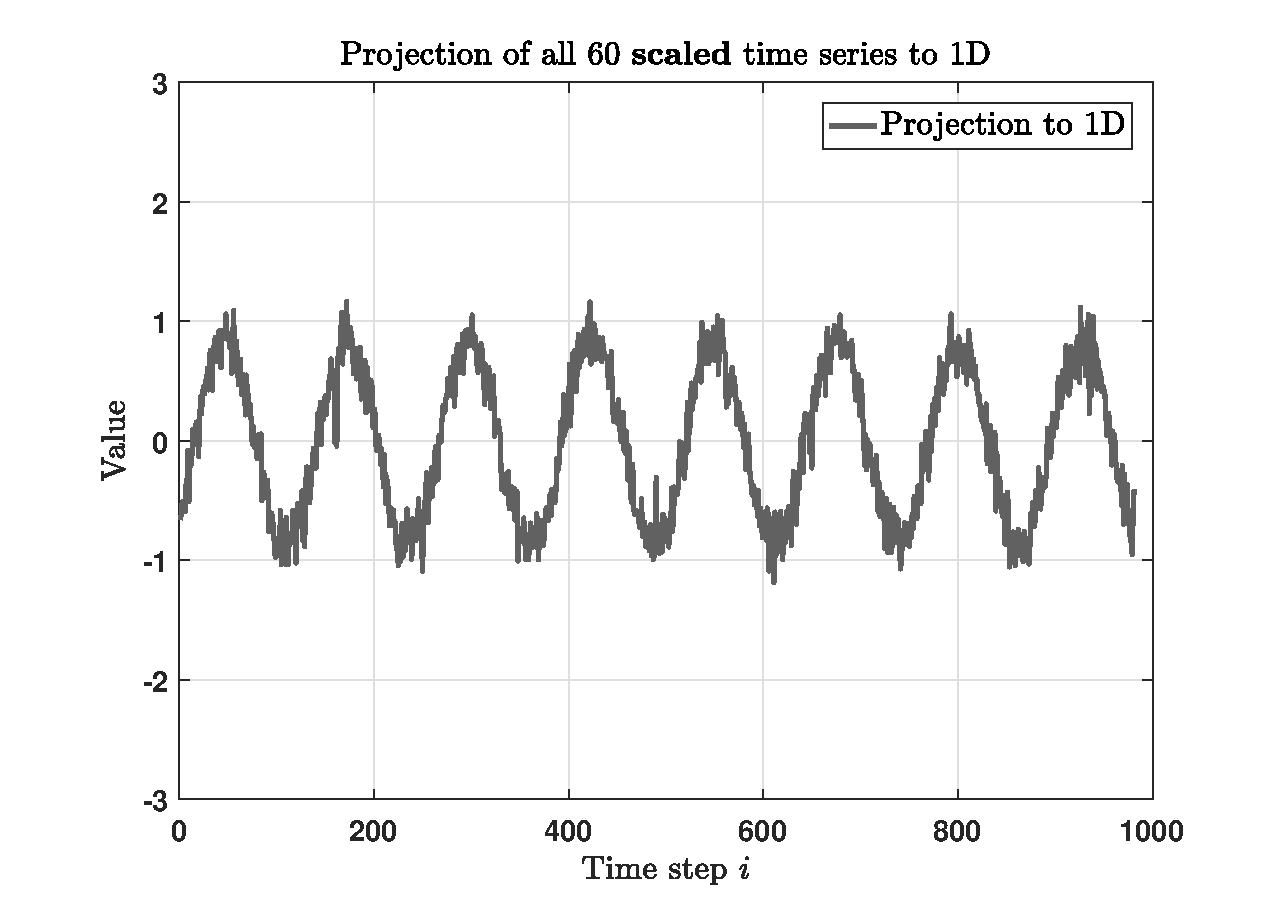
\includegraphics[scale=0.345]{analysis/Analysis_scaled_projection}
	\vspace{-0.12cm}
	\caption{Projections of the $60$D unstandardized (left) and standardized (right) time series to $1$D.}
	\label{fig:analysis_innerworking_projection}
	\vspace{-0.25cm}
\end{figure}

The principal sinusoidal behaviour can be clearly seen in both projections. We can also still see reflections of the outliers in the resulting projections at for instance $i \approx 500$. The obtained projections are reconstructed to what is shown in figure \ref{fig:analysis_innerworking_reconstruction}. Logically, the reconstructed time series all are in-phase with the $1$D projection. This causes the original time series and their reconstructions to be out-of-phase, resulting in misalignment. Again, to avoid occlusion figure \ref{fig:analysis_innerworking_reconstruction} only shows a subset of $12$ time series out of the $60$ input time series.

\begin{figure}[h]
	\centering
	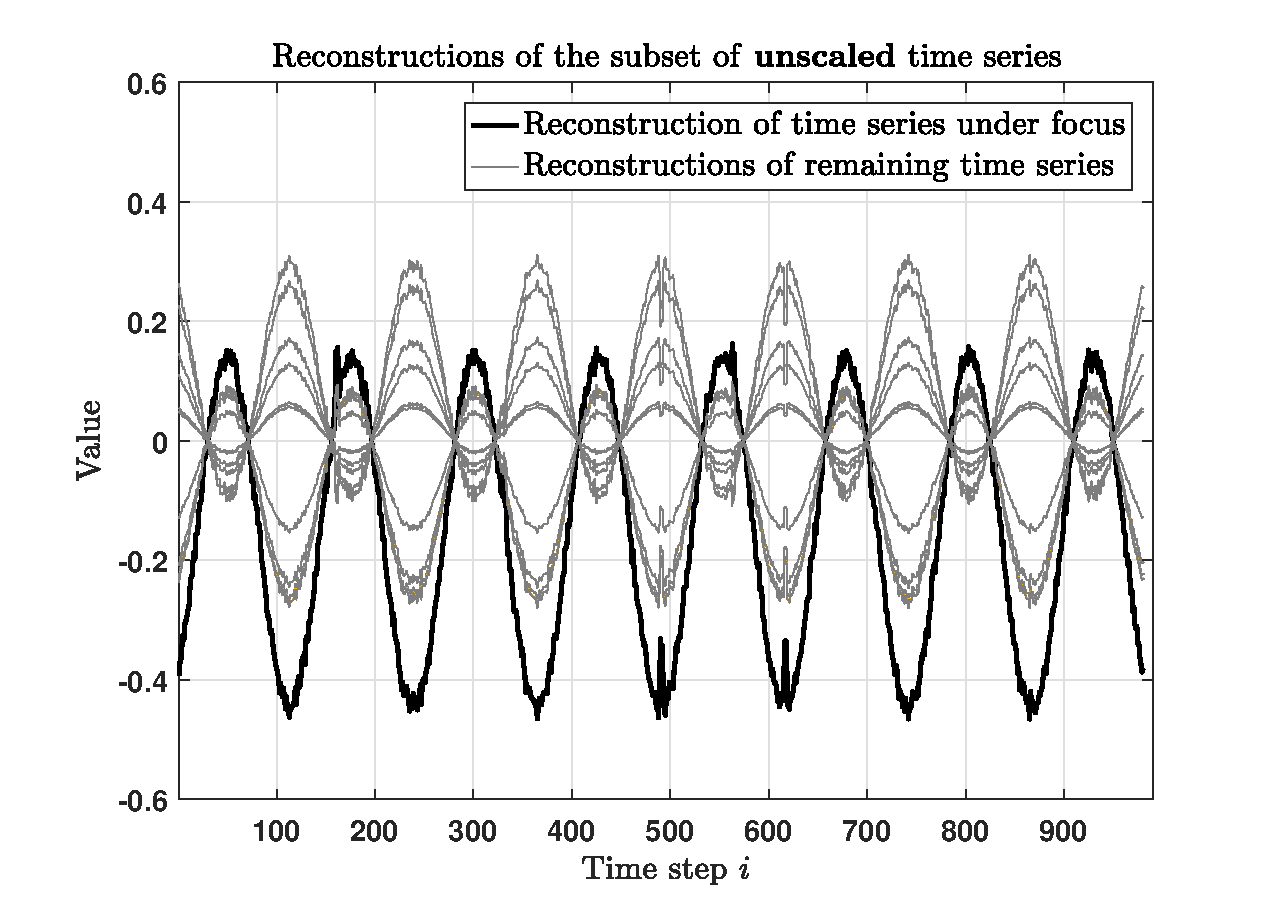
\includegraphics[scale=0.36]{analysis/Analysis_unscaled_reconstruction}
	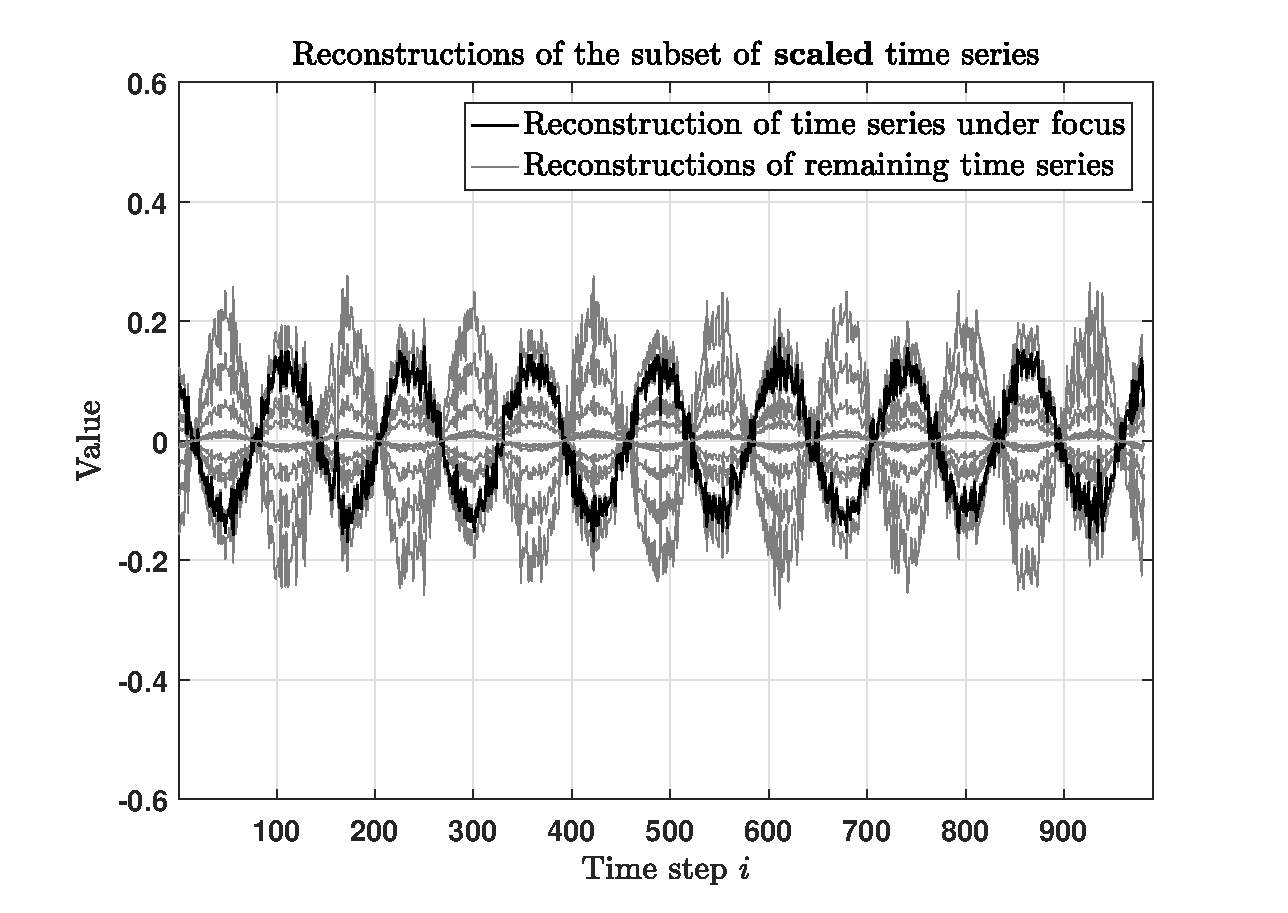
\includegraphics[scale=0.36]{analysis/Analysis_scaled_reconstruction}
	\caption{Reconstructions of unstandardized (left) and standardized (right) subset of time series.}
	\label{fig:analysis_innerworking_reconstruction}
	\vspace{-0.15cm}
\end{figure}

\newpage
The consequence of our misaligned reconstructions can be clearly recognized in the obtained outlier scores as shown in figure \ref{fig:analysis_innerworking_outlierscores}. Also note that the means of the reconstructed unstandardized time series are closer to $0$ than the means of the original time series, while the means of the reconstructed standardized time series remain $0$. Due to the larger difference in mean and range between an unstandardized time series and its reconstruction, we might be unlucky and not find the global point outliers at $i \approx \{170, 330, 570\}$, as shown at the left-hand side of figure \ref{fig:analysis_innerworking_outlierscores}. If we standardize the data we do not suffer from this as shown at the right.

\begin{figure}[h]
	\centering
	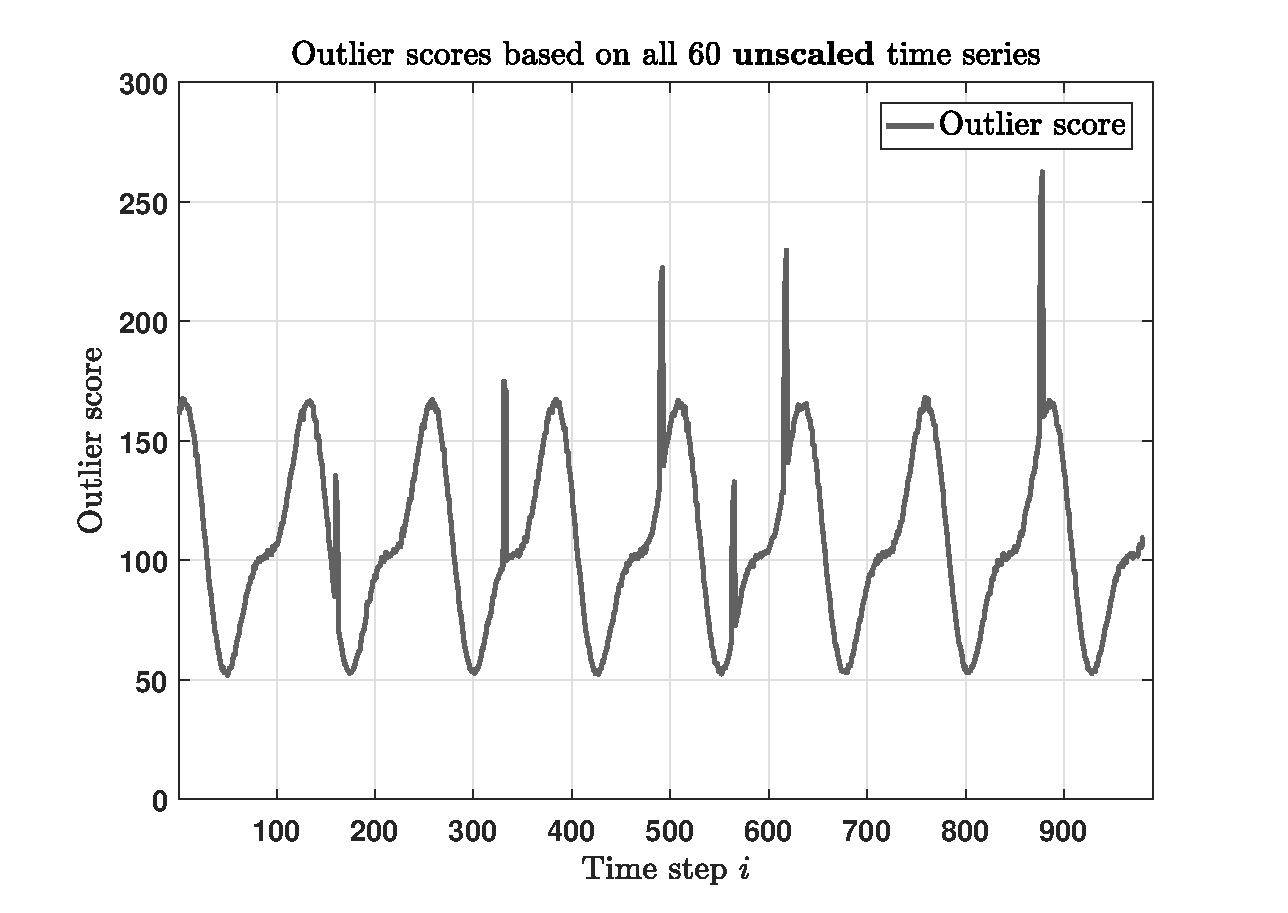
\includegraphics[scale=0.36]{analysis/Analysis_unscaled_outlierscores}
	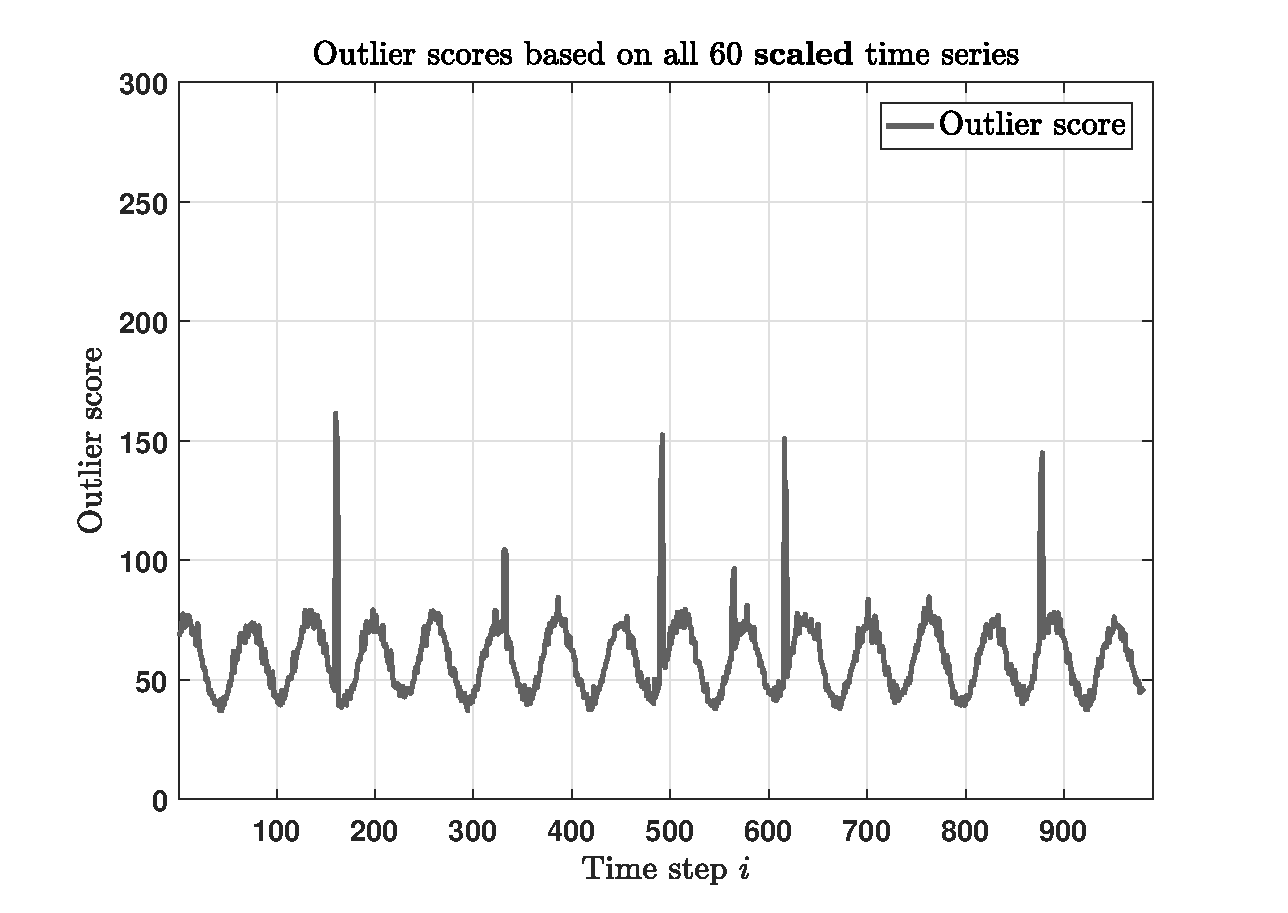
\includegraphics[scale=0.36]{analysis/Analysis_scaled_outlierscores}
	\caption{Outlier scores of unscaled (left) and scaled (right) time series.}
	\label{fig:analysis_innerworking_outlierscores}
\end{figure}

For contextual point and collective outliers we have exactly the same results up to the outlier scores. That is, due to the contextualness of these outlier types, the original time series at those time steps are likely closer to the reconstructed data points, as explained in chapter \ref{chap:rp-method}. Back-scaling in some cases resolves this problem, but certainly not always as will become clear in section \ref{sec:analysis_bird}.
Finally, it is important to realize that the RP method relies on the correlation among the different time series. To that end, the RP method does not find outliers that cause all time series to show significant deviations considering their normal behaviours. This certainly is a limitation of the method.


\section{A bird's-eye view}
\label{sec:analysis_bird}

In this section we focus on the behaviour of the detection and runtime performances of the RP method and its baseline SPIRIT under varying parameter settings. 
We investigated these behavioural properties for the $3$ different outlier types, window lengths $p = \{1,5,10,15\}$, and for the number of projection vectors $k$ from $1 \text{ to } 25$. For SPIRIT we have the forgetting factor $\lambda$ as additional parameter which we have set to $0.97$ being within the typical range of $[0.96, 0.98]$ \cite{papadimitriou2005streaming}. We also used these experiments to determine the influence of back-scaling with factor $\sqrt{\frac{d}{k}}$ on the detection performance. Therefore, we ran all experiments in this section with both versions of the RP method: with and without back-scaling. 

\begin{figure}[h]
	\centering
	\vspace{-0.1cm}
	\includegraphics[scale=0.35]{analysis/AUCs_point}
	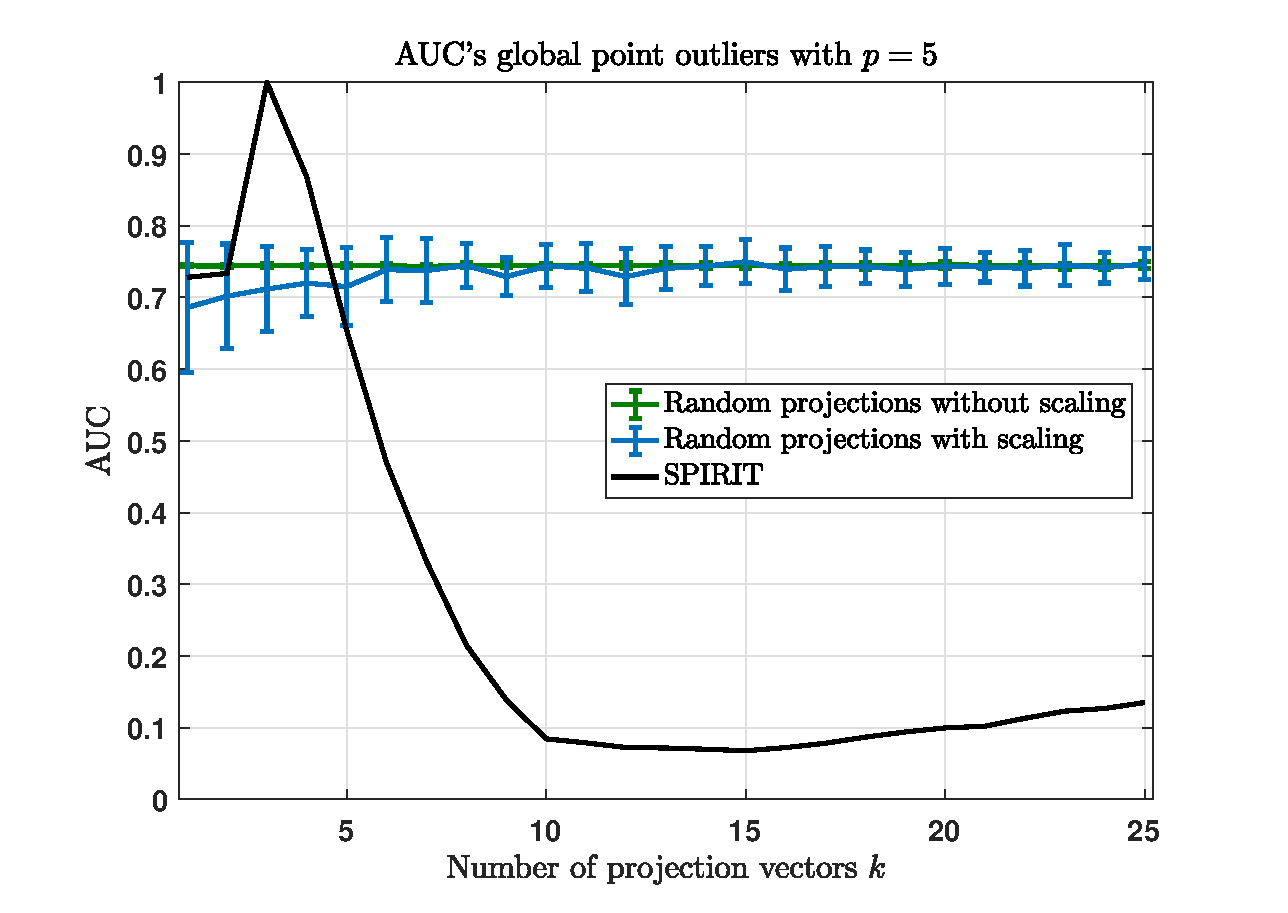
\includegraphics[scale=0.35]{analysis/AUCs_point1}\\
	\includegraphics[scale=0.35]{analysis/AUCs_point2}
	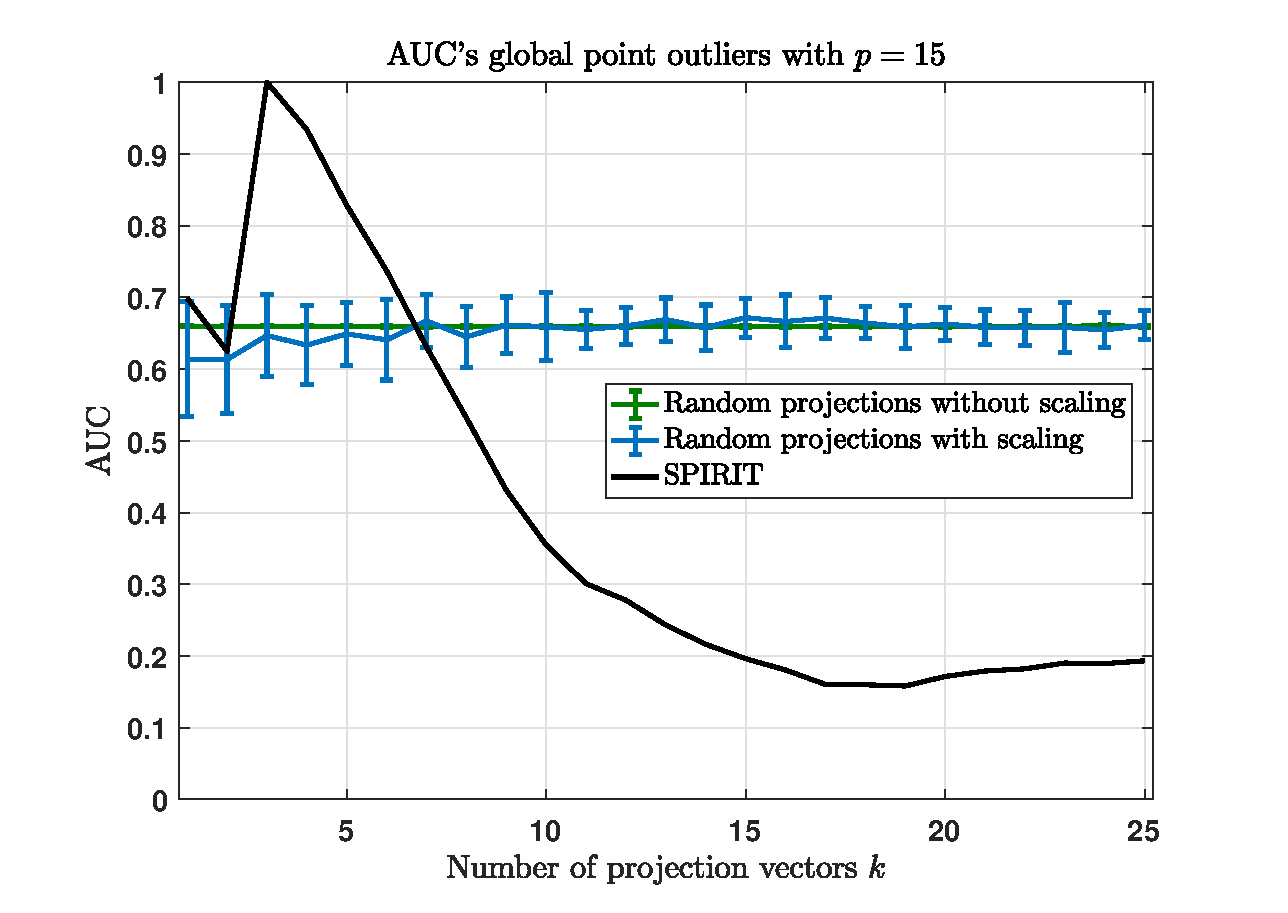
\includegraphics[scale=0.35]{analysis/AUCs_point3}
	\caption{Detection performances of global point outliers with $k$ from $1$ to $25$ and $p=\{1,5,10,15\}$.}
	\label{fig:analysis_aucs_point}
	\vspace{-0.26cm}
\end{figure}

Starting with figure \ref{fig:analysis_aucs_point}, we present the detection performances for global point outliers. It becomes clear that the AUC of SPIRIT is very sensitive to the number of projection vectors ($k$) used, as expected. SPIRIT yields a clear peak in AUC at $k=3$ where the AUC is $1$ regardless of the sliding window size, which translates to a $100\%$ chance of correctly labelling a randomly selected pair of a normal data point and an outlier. Yet the AUC drops at a high rate after adding more projection vectors. Considering the performance without a sliding window ($p=1$), the AUC even drops from $1$ to $0.1$ between $k=3$ and $k=5$ which implies that the $4^{\text{th}}$ and $5^{\text{th}}$ principal components align well with the outliers. The detection performance of the RP method with and without back-scaling is relatively insensitive to the number of projection vectors $k$ and results in an AUC around $0.9$ irrespective of $k$. The RP method without back-scaling reaches an AUC slightly higher and more stable than with back-scaling, as was expected. The RP method basically benefits from the power of the squared Euclidean distance to emphasize very large reconstruction errors (from outliers) in contrast to `just' large reconstruction errors (corresponding to normal data points).

Clearly, the advantage of stability is therefore on behalf of the random projection methods. If we would know on forehand what a proper $k$ would be for the entire stream, SPIRIT has potential to yield a very high AUC. Unfortunately it is often unknown what to expect, where the behaviour of systems is likely not as stable as our synthetic sinusoidal time series. Even if we could make an educated guess to what a sufficient value for $k$ might be, if reality deviates a little from our guess we might completely miss the principal behaviour or reconstruct our outliers better. Implementing SPIRIT with a sliding window makes the performance less sensitive to $k$, which might be sufficient to get a generally well performing method. The RP method does not benefit from a window, and even makes it perform worse.

Though we only based our expectations regarding the effects of back-scaling on loose reasoning, scaling $\hat{\mathbf{x}}_i$ back to approximate the data point its original norm results in a less stable and often worse performance compared to its not back-scaled counterpart. Another difference between the two variants of the RP method we would like to emphasize, is that the AUC of the method without back-scaling slightly decreases when more projection vectors are added in contrast to its scaled version. Throughout all (preliminary) experiments with this method, we remarkably found that for the RP method without back-scaling taking $k=1$ on average performs better than taking $k=2$ or $k=3$, etcetera, regardless of the data at hand. We elaborate on this observation in more detail in section \ref{sec:analysis_contextual}.

When it comes to comparing runtime performances, the proposed method outperforms SPIRIT heavily. Figure \ref{fig:analysis_runtimes_point} shows the runtime performances associated with the discussed detections. We are confirmed that even for $k=1$ SPIRIT runs twice as slow as the random projection method. This reveals the difference in the hidden constants behind the upper bounds on the computational complexity of the RP method and SPIRIT. That is, for $k=1$ we have no influence of the quadratic factor on the runtime of SPIRIT, yet its runtime is twice as high as from the RP method. Therefore, its upper bound is closer to $\mathcal{O}(2k^2d)$ compared to $\mathcal{O}(kd)$ of the RP method.

\begin{figure}[h]
	\centering
	\vspace{0.25cm}
	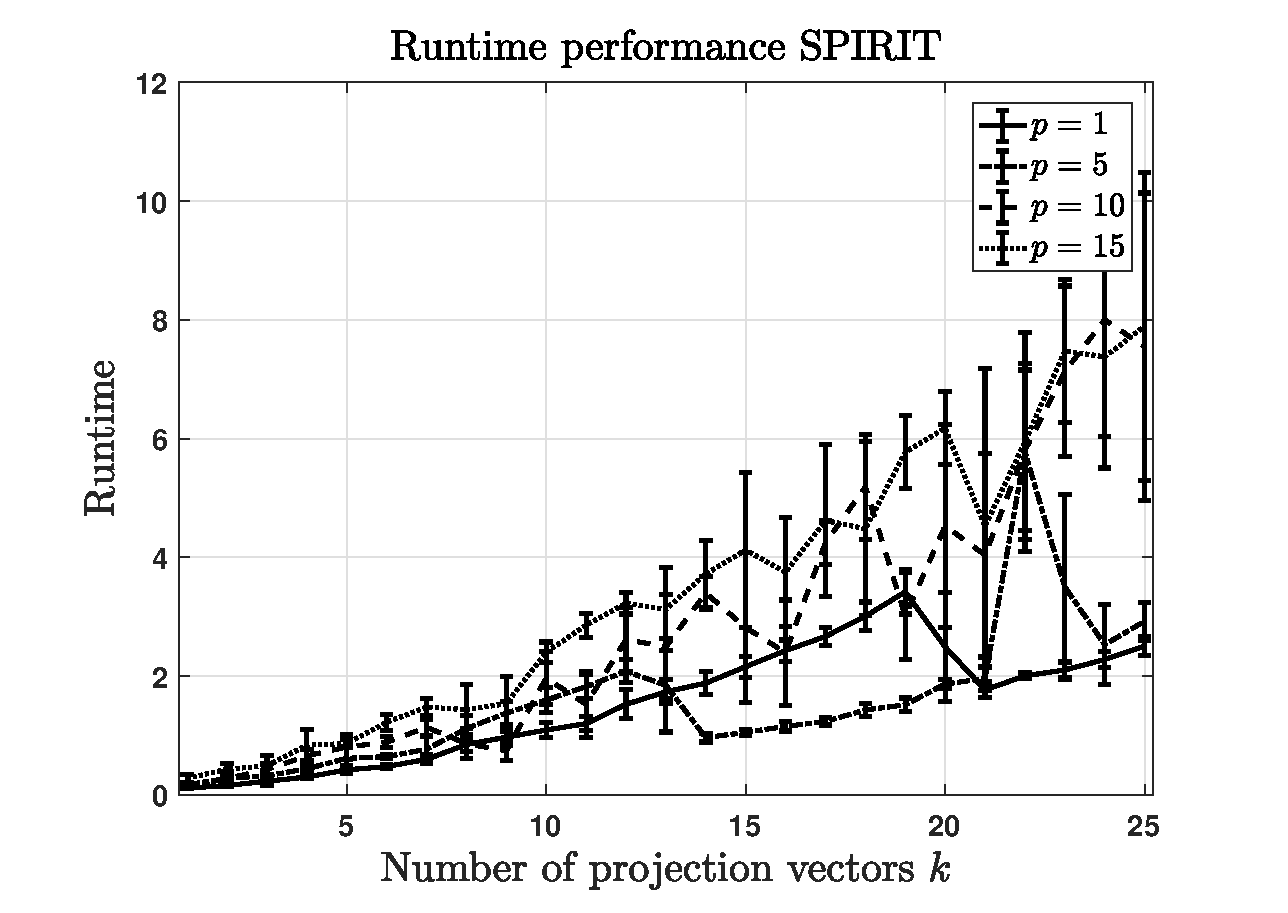
\includegraphics[scale=0.36]{analysis/Runtimes_SPIRIT_point}
	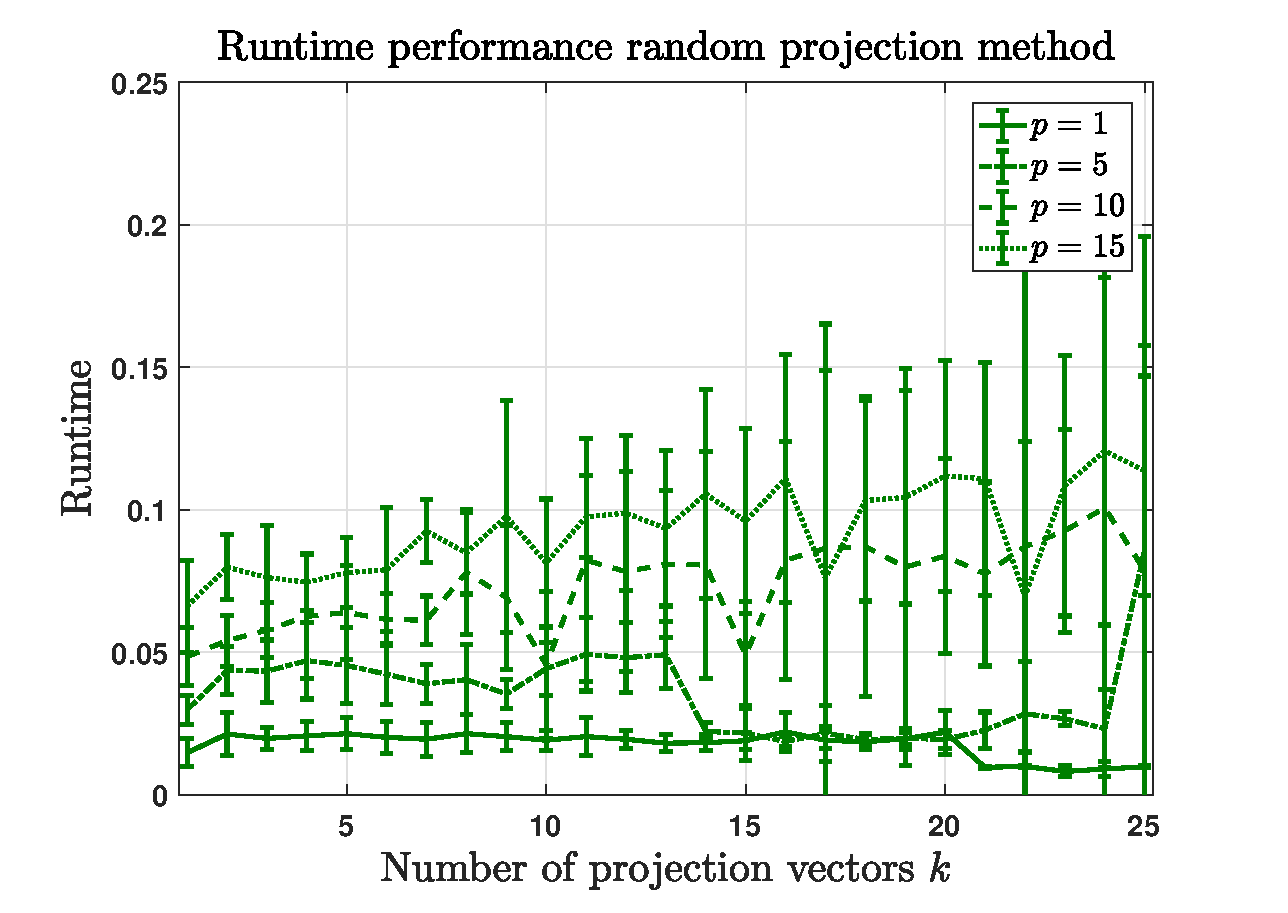
\includegraphics[scale=0.36]{analysis/Runtimes_RP_point}
	\vspace{0.1cm}
	\caption{Runtime performances of global point outliers with $k$ from $1$ to $25$ and $p=\{1,5,10,15\}$.}
	\label{fig:analysis_runtimes_point}
	\vspace{0.25cm}
\end{figure}

From figure \ref{fig:analysis_aucs_contextual} (left) it becomes clear that the RP method is less successful for finding contextual outliers. For contextual point outliers (left) it even results in stable AUC's around $0.3$, making it perform worse than random guessing the labels of a randomly selected pair of a normal data point and an outlier. Contextual collective outliers (right) are only detected a little better than random guessing. The remaining patterns compared to SPIRIT are quite similar to the observations made previously.

\begin{figure}[h]
	\centering
	\vspace{0.25cm}
	\includegraphics[scale=0.36]{analysis/AUCs_contextual}
	\includegraphics[scale=0.36]{analysis/AUCs_collective}
	\vspace{0.1cm}
	\caption{Detection performances of contextual point and collective outliers with $k$ from $1$ to $25$ for $p=1$.}
	\label{fig:analysis_aucs_contextual}
	\vspace{0.25cm}
\end{figure}

This poor performance is a direct consequence of the feature values of such outliers, which in most cases are closer to the reconstructed model than the remainder of the data points. This effect is illustrated in figure \ref{fig:analysis_contextualreconstruction} for the reconstruction with the RP method with and without back-scaling, where we used $15$ projection vectors and no sliding window. In this example the outliers are also reconstructed relatively good which is an undesired outcome as well.

\begin{figure}[h]
	\centering
	\vspace{0.1cm}
	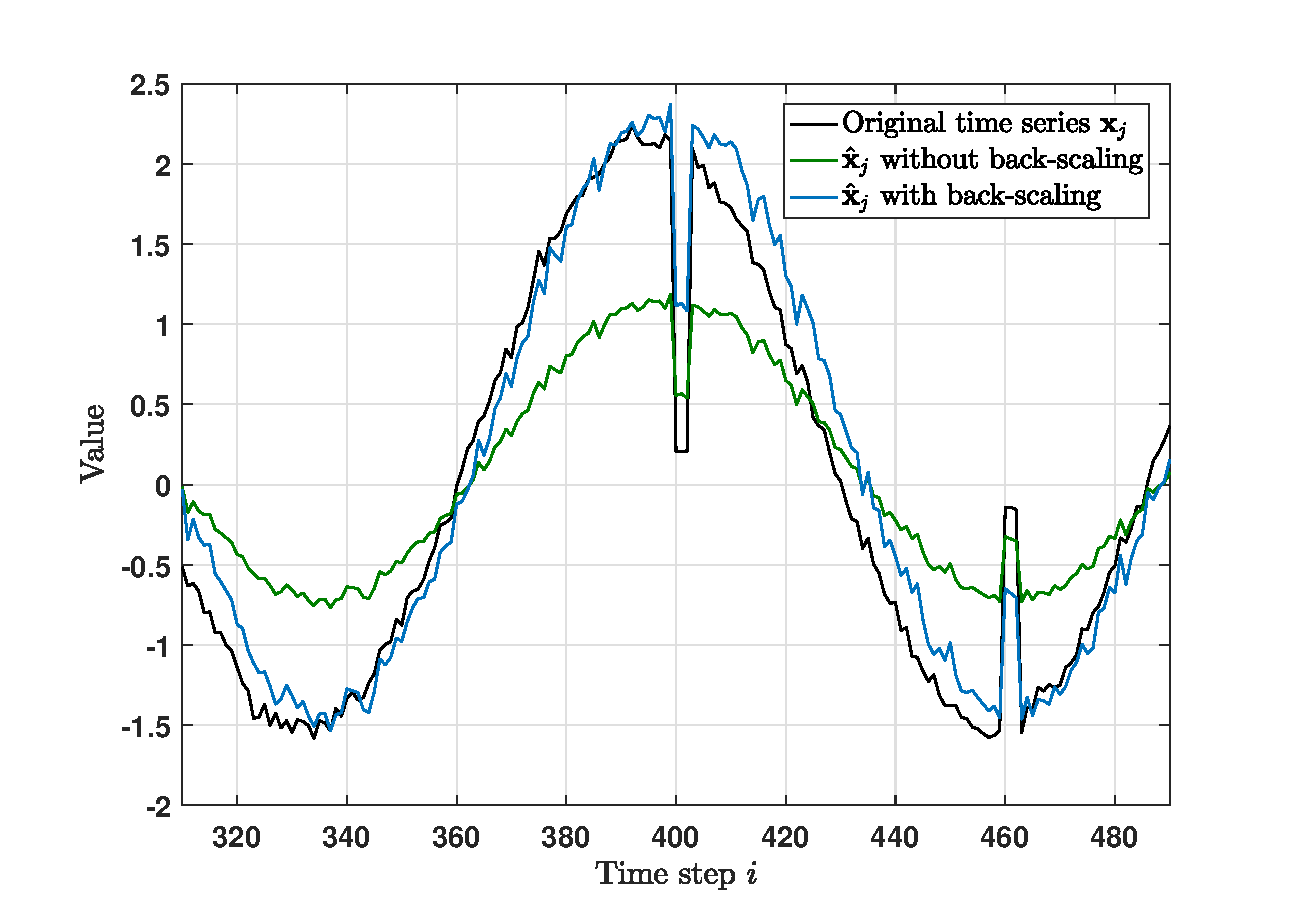
\includegraphics[scale=0.38]{analysis/Analysis_contextualreconstructionrp}
	\caption{Reconstruction of a time series with contextual outliers with $k=15$ projection vectors.}
	\label{fig:analysis_contextualreconstruction}
\end{figure}

\newpage
The squared Euclidean distances between the reconstructions of outliers and their original values are then typically smaller, resulting in reconstruction errors lower than or equal to the reconstruction errors of normal data points. Back-scaling does play an important role for finding contextual outliers as the model behaviour is then more often closer to the original behaviour, as can be derived from figure \ref{fig:analysis_contextualreconstruction} as well. However, scaling the reconstructed data point back does not significantly improve the detections which becomes clear from the AUC's in figure \ref{fig:analysis_aucs_contextual}. 

The detection performances associated with window lengths $p=\{5,10,15\}$ can be found in appendix \ref{app:analysis}. From these experiments, we found that a sliding window only helps a little for the detection of contextual outliers. Yet we need a window length $p$ of approximately $15$ data points to obtain an AUC around $0.5$ for contextual point outliers. As the runtime performances are independent of the type of outliers in the data, the runtime performances are similar to what has been shown in figure \ref{fig:analysis_runtimes_point} and therefore are not presented.

With or without back-scaling and adopting a sliding window or not, deriving outlier scores from reconstructions from random projections does not have a high potential for contextual outliers. \\

\noindent In short, we observed the following from this analysis:
\begin{itemize}
	\itemsep-0.2em
	\item The RP method performs competitive AUC-wise when the outliers are global, but SPIRIT is more successful in finding outliers of all three types.
	\item The RP method without back-scaling results in a less accurate model of the original data but yields a more stable performance for all outlier types. The back-scaled version, however, is slightly better at detecting contextual outliers.
	\item The detection performance of the RP method is stable for varying number of projection vectors $k$ and often obtains its optimal performance for $k=1$. Therefore, taking $k=1$ would be a generally safe option making this method parameter-free.	
	\item The detection performance of SPIRIT is highly sensitive to the number of projection vectors $k$.
	\item The RP method does not benefit from a window and by default does not exploit temporal relations over time. 
	\item SPIRIT benefits from a window as it reduces its sensitivity of the detection performance to $k$.
	\item The runtime of the RP method is low and only linearly depending on $k$.
	\item SPIRIT is tractable if the data is highly correlated or low dimensional due to the low number of projection vectors needed in those cases. If more vectors are needed to explain the desired variance, this method becomes expensive as its runtime quadratically depends on $k$.
\end{itemize}

Two observations are particularly interesting: the RP method yields very poor results for contextual outliers, but reaches its optimal operating point for $k=1$. In the next section we elaborate more on these conclusions.


\section{Detecting contextual outliers}
\label{sec:analysis_contextual}

Contextual outliers are most often misclassified if we assign outlier scores as in algorithm \ref{alg:analysis_algorithm}. This is caused by the feature values of such outliers, which are closer to the values of the reconstructed data point. This results in a lower reconstruction error than for normal data points, hence resulting in AUC's lower than $0.5$. Missing them can be critical for outlier detection in multivariate time series as contextual outliers might appear in the data.

One solution to detect the contextual point outliers more accurately is by taking the inverse of the outlier scores ($\frac{1}{O_i}$) such that the labels are reversed. Doing so would not significantly affect the runtime performance. However, it would obviously not be effective for finding global point outliers, or contextual collective outliers for which the AUC's then will be lower than $0.5$. We could take the maximum of the combination of the original outlier scores and their inverses instead. Unfortunately, we would not get an AUC higher than around $1 - 0.3 = 0.7$ this way for contextual point outliers.

Another observation was that we often detect outliers better with only one projection vector than when we use multiple, regardless of the type of outliers. That is, the RP method yields on average its optimal AUC with $k=1$ and therefore is higher than with $k=1+\Delta$.
Recall, that we assign outlier scores directly from reconstruction errors. Linking this to our observation, it can be concluded that we can separate outliers from normal data points worse by their reconstruction errors, when we increase the number of projection vectors $k$. This would imply that the outliers are reconstructed better at a faster rate than normal data points are after adding a random projection vector to the projection matrix. 
This brings us to the formulation of hypothesis \ref{hyp:analysis_outlierinlier}.


\begin{hypothesis}\label{hyp:analysis_outlierinlier}
	For $k, \Delta > 0$, let $\mathbf{X}$ be an arbitrary data set of size $d \times n$ with sufficiently correlated features.
	Then with high probability we have for all $\mathbf{x} \in \mathbf{X}$:

	\[ |\mathcal{E}_{k,\text{normal}} - \mathcal{E}_{k+\Delta,\text{normal}}| \ < \ |\mathcal{E}_{k,\text{outlier}} - \mathcal{E}_{k+\Delta,\text{outlier}}| \]
	
	\vspace{0.2cm}
	
	\noindent with $\mathcal{E}_{k,\mathbf{x}}$ the reconstruction error of data point $\mathbf{x}$ obtained with the RP method.
\end{hypothesis}

Though it would be interesting to formally prove hypothesis \ref{hyp:analysis_outlierinlier}, in this thesis we focus on exploiting it to find contextual outliers besides global outliers. But, how can we do this?
Going back to the fundamental objective of outlier detection methods, we aim at assigning higher outlier scores to outliers than to normal data points. Such a relation between normal data points and outliers follows directly from our hypothesis. If hypothesis \ref{hyp:analysis_outlierinlier} holds and we compute the outlier scores as 

\begin{equation}\label{eq:hypothesis_outlierscores}
	O_i \gets |\| \mathbf{x}_i - \hat{\mathbf{x}}_i \|^2_{k} - \| \mathbf{x}_i - \hat{\mathbf{x}}_i \|^2_{k+\Delta}|,
\vspace{0.1cm}
\end{equation}

\noindent we would get higher outlier scores for outliers than for normal data points.\\
Unfortunately, this introduces two drawbacks. First, we might end up projecting in such a way that we reconstruct our outliers better which happens with an unknown probability. To avoid these occurrences we can rely on taking the maximum of $m$ distinct predictions for $O_i$. Sadly, this introduces a parameter, $m$ the number of predictors and increases the runtime. 

Second, the resulting reconstruction errors are likely in a different range. This issue can be resolved by standardizing the reconstruction errors obtained with $k$ and $k+\Delta$ projection vectors. By standardizing the outlier scores of the predictors, they get $0$ mean and unit variance. It is not tractable to keep a large window of the stream in memory to compute the mean and standard deviation at each time step $i$, which also would introduce this window length as an additional parameter. Therefore, we only track a few scalars estimating these statistics following equations \eqref{eq:analysis_online_mean} to \eqref{eq:analysis_online_std}, for which thorough derivations can be found in \cite{finch2009incremental}.


\begin{equation}\label{eq:analysis_online_mean}
	\mu_i = \mu_{i-1} + \frac{\mathbf{z}_i - \mu_{i-1}}{i}
\end{equation}

\begin{equation}\label{eq:analysis_online_var}
	S_i = S_{i-1} + (\mathbf{z}_i - \mu_{i-1}) \ (\mathbf{z}_i - \mu_i)
\end{equation}

\begin{equation}\label{eq:analysis_online_std}
	\sigma_i = \sqrt{\frac{S_{i}}{i}}
\end{equation}

Note, that these equations only reflect the estimation of the mean and standard deviation of one outlier score vector $\mathbf{z}$ over time. However, we also need to standardize the set of $m$ predictions for each data point over time ($\mathbf{O}_{\text{stand},m}$), so we have $m$ such means and standard deviations for this set over time. We refer to the low-cost online standardization procedure as stand($\mathbf{z}_i$). The resulting adjusted interpretation of outlier scores generated by the RP method is summarized in algorithm \ref{alg:analysis_algorithm_delta}. We refer to this interpretation as $\Delta$RP.

\vspace{-0.2cm}	
\begin{algorithm}[H]
	\caption{\quad \textbf{$\Delta$RP}}
	\label{alg:analysis_algorithm_delta}
	\begin{flushleft}
	\vspace{-0.2cm}
	\textbf{Input} data point $\mathbf{x}_i$ of size $d \times 1$\\
	\textbf{Input} number of predictors $m$	
	\vspace{-0.1cm}
	\end{flushleft}
	\begin{algorithmic}[1]	
		\vspace{-0.2cm}
		\STATE Initialize set of predictors $\mathbf{O}_{\text{stand},m}$ as $\emptyset$
		\FOR{$j$ in $m$ predictors}
			\STATE $O_{1,j} \gets \text{RP}(\mathbf{x}_i, k=1)$
			\STATE $O_{2,j} \gets \text{RP}(\mathbf{x}_i, k=2)$
			\STATE Add $\text{stand}(|\text{stand}(O_{1,j}) - \text{stand}(O_{2,j})|)$ to $\mathbf{O}_{\text{stand},m}$
		\ENDFOR
		\STATE $O_i = \max \{\mathbf{O}_{\text{stand},m}\}$
	\end{algorithmic}
	\begin{flushleft}
	\vspace{-0.3cm}
	\textbf{Output} outlier score $O_i$
	\vspace{-0.3cm}
	\end{flushleft}
\end{algorithm}
\vspace{-0.2cm}

As we are particularly interested in the detection performance of $\Delta$RP with respect to contextual outliers, we illustrate the inner working of this method by means of the data with contextual point outliers. Again, we only show a subset of $12$ time series instead of all $60$ time series to avoid occlusion. Figure \ref{fig:analysis_example_original} shows the time series we focus on throughout this example in the context of these $12$ time series.

\begin{figure}[h]
	\centering
	\vspace{-0.15cm}
	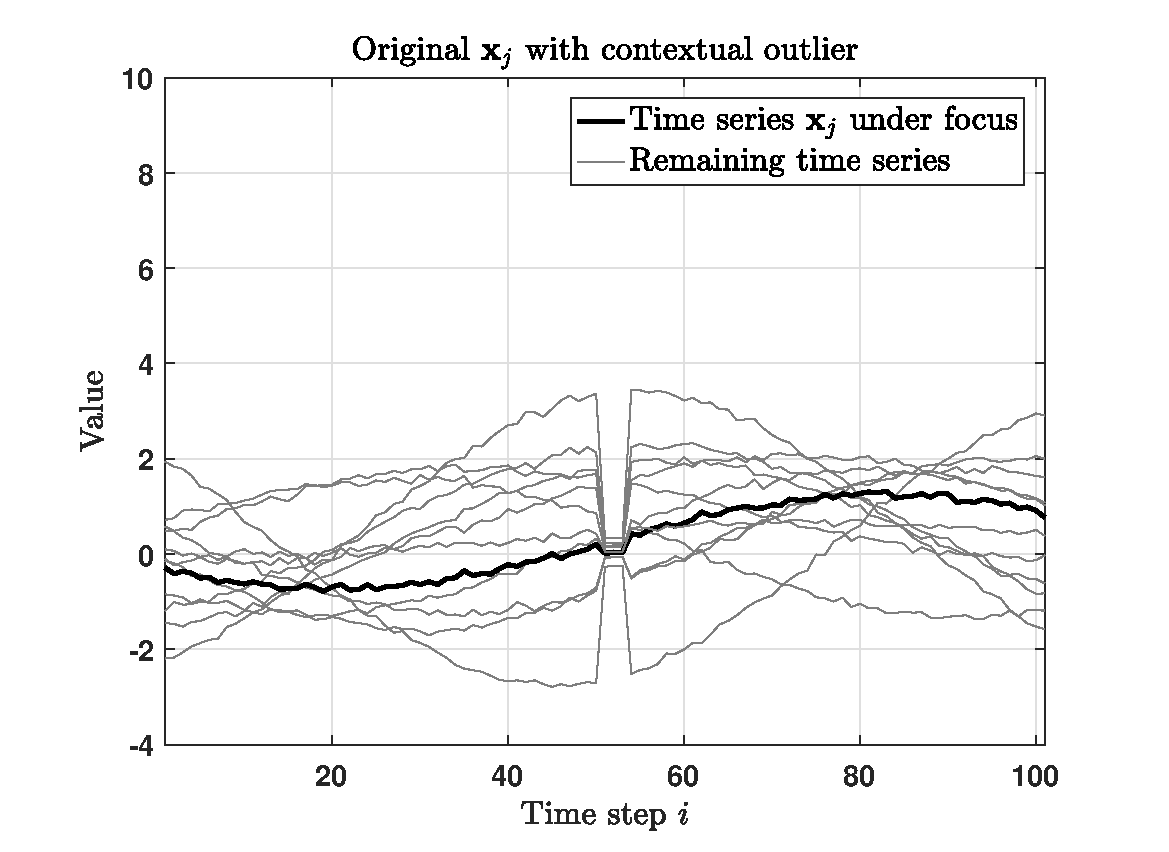
\includegraphics[scale=0.35]{analysis/Analysis_deltarp_original}
	\caption{Original subset of time series with contextual outliers.}
	\label{fig:analysis_example_original}
	\vspace{-0.15cm}
\end{figure}

The original $60$ time series are then projected once into $1$ and once into $2$ random directions with the default RP method as formulated in algorithm \ref{alg:analysis_algorithm}. Figure \ref{fig:analysis_example_projections} shows the resulting $1$D (left) and $2$D projection (right). The figure corresponding to the projection with $k=2$ (right) illustrates how projecting the data into two approximately orthogonal directions likely yields a better reconstruction of the outliers than when projecting in only $1$ random direction. 

\begin{figure}[h]
	\centering
	\vspace{-0.15cm}
	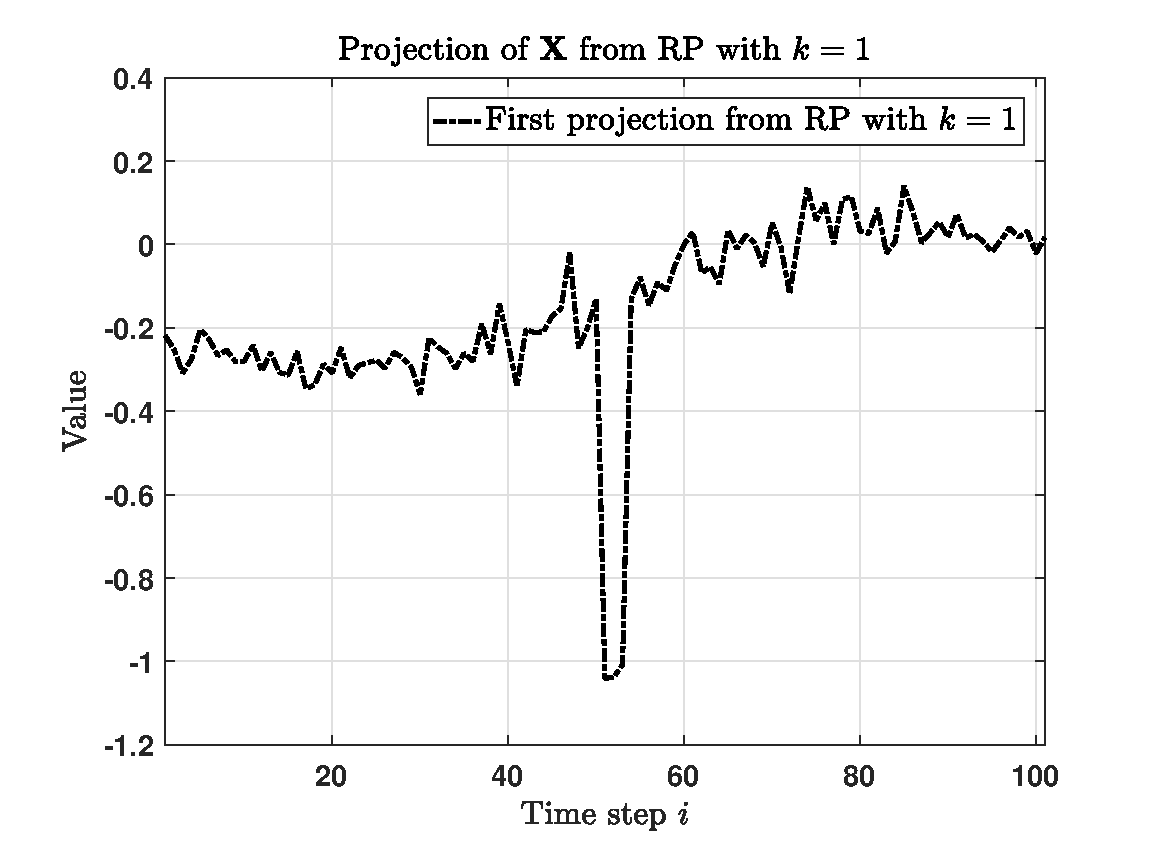
\includegraphics[scale=0.35]{analysis/Analysis_deltarp_projection1}
	\includegraphics[scale=0.35]{analysis/Analysis_deltarp_projection2}
	\caption{Projections of RP with $k=1$ (left) and $k=2$ (right).}
	\label{fig:analysis_example_projections}
	\vspace{-0.3cm}
\end{figure}

Figure \ref{fig:analysis_example_reconstructions} (left) shows what happens when we reconstruct the projections from the $1$D and $2$D projections. Despite the misalignment caused by the distinct random directions, it becomes clear that the reconstruction of the outlier around $i=500$ with $k=2$ is much closer to the original data point compared to $k=1$ which shows a high peak around $i=500$. This in turn results in a larger absolute difference between the two reconstructions of the outlier obtained with $k=1$ and $k=2$ than between the reconstructions of the normal data points surrounding this outlier (right). 

\begin{figure}[h]
	\centering
	\vspace{0.15cm}
	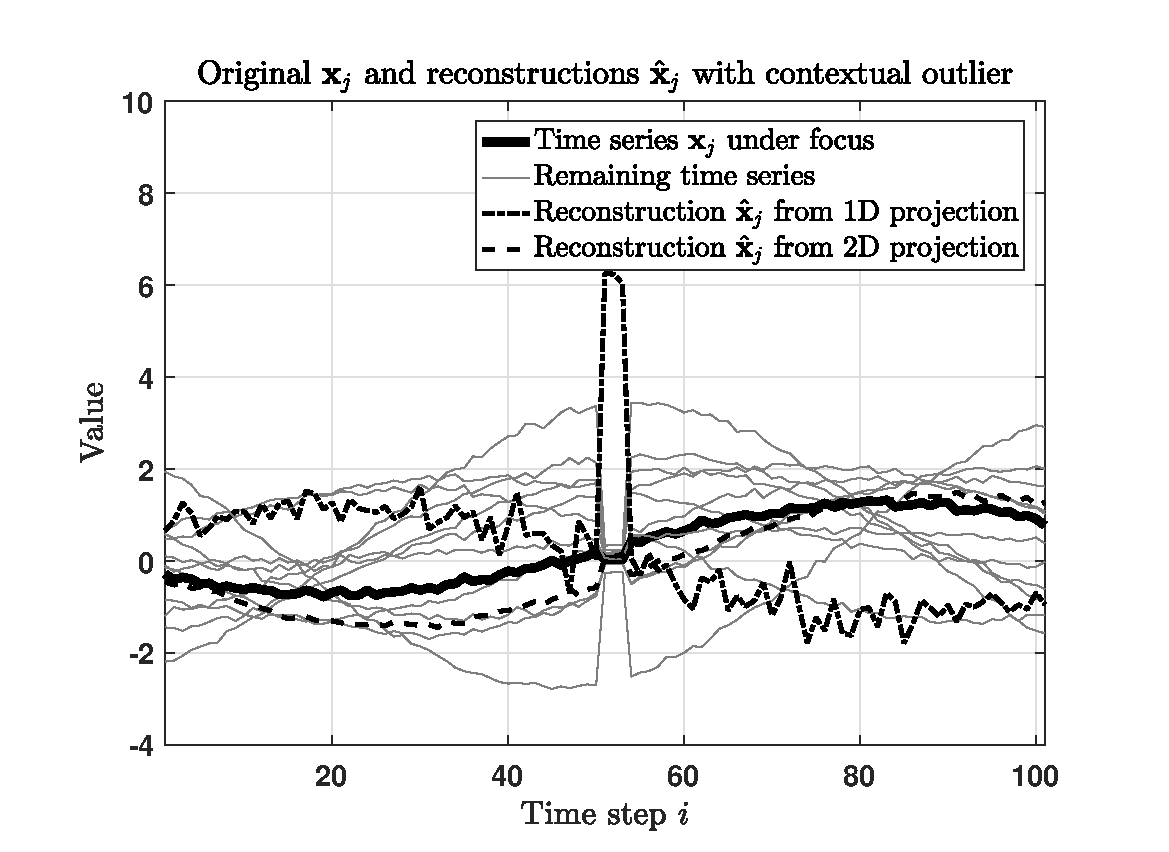
\includegraphics[scale=0.36]{analysis/Analysis_deltarp_original_reconstructions}
	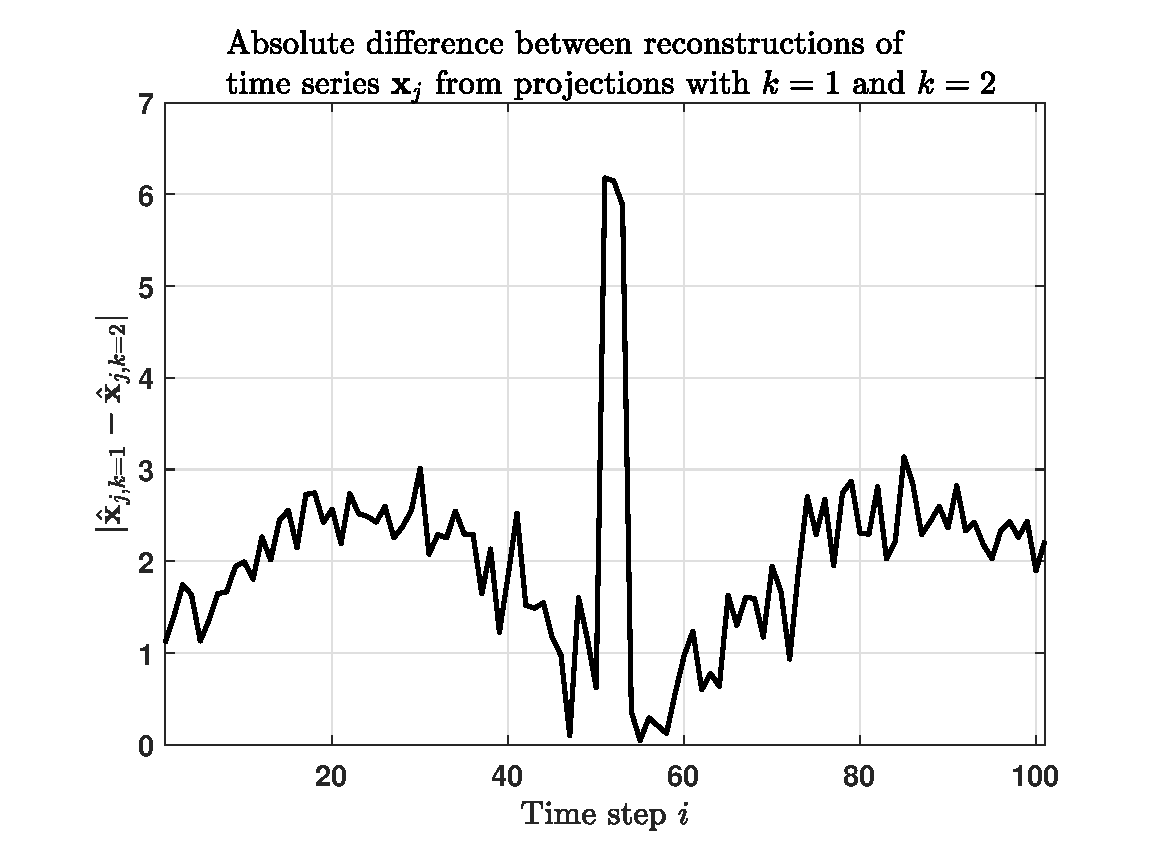
\includegraphics[scale=0.36]{analysis/Analysis_deltarp_diffreconstructions}
	\caption{Example reconstructions of time series with $k=1$ and $k=2$ (left) and corresponding absolute difference (right).}
	\label{fig:analysis_example_reconstructions}
	\vspace{0.15cm}
\end{figure}

As we have one (other) parameter to set for $\Delta$RP, $m$ the number of predictors for $O_i$, we can observe its performance for $m$ from $1$ to $25$ against SPIRIT for which we observe its performance for the number of projection vectors $k$ from $1$ to $25$ as well. This analysis has also been conducted on the standardized data of which the results are presented and discussed in appendix \ref{app:analysis}. Figure \ref{fig:analysis_aucs_global_spiritdelta} shows the results of the experiments for detecting global point outliers.

\begin{figure}[h]
	\centering
	\vspace{0.15cm}
	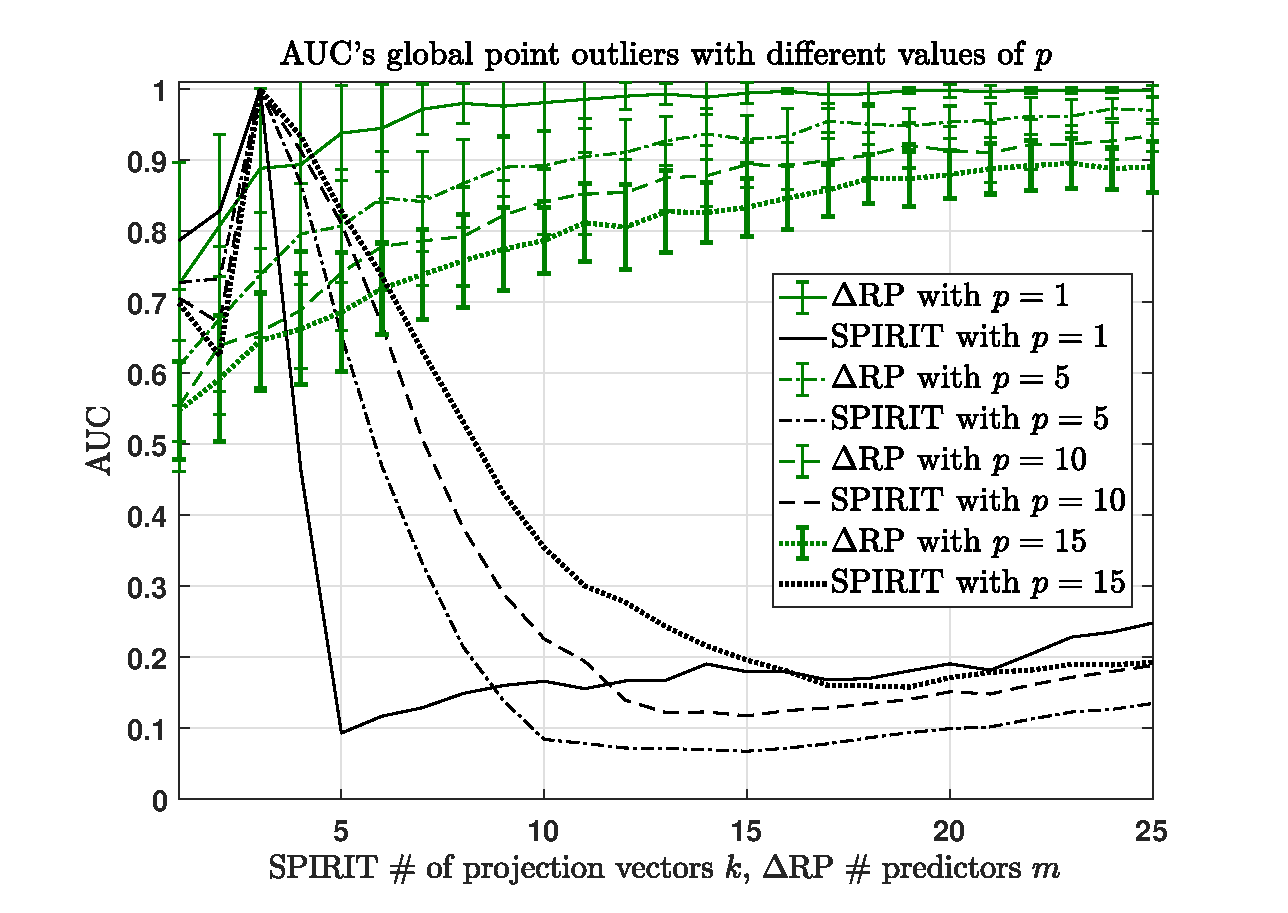
\includegraphics[scale=0.36]{analysis/AUCs_point_spiritdelta}
	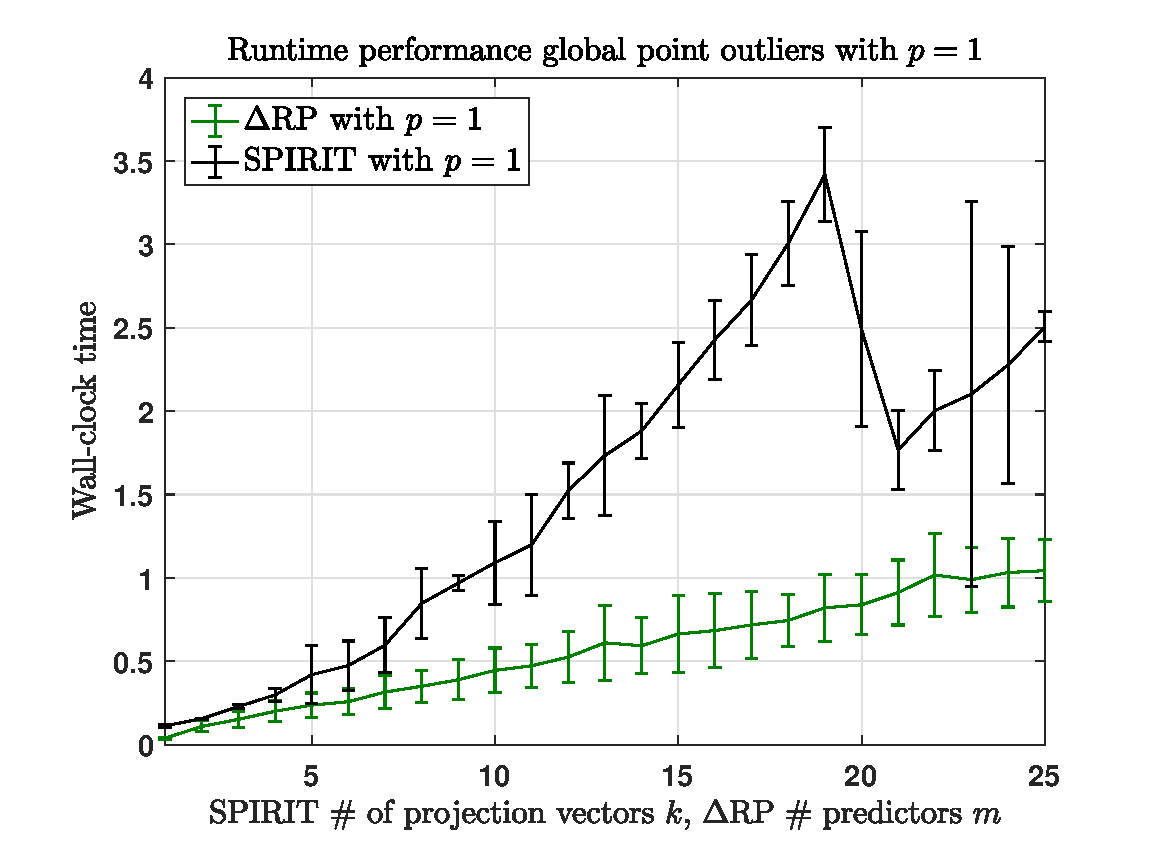
\includegraphics[scale=0.38]{analysis/Runtimes_point_spiritdelta}
	\caption{Detection and runtime performances of global point outliers with $k$ and $m$ from $1$ to $25$ for $p=\{1,5,10,15\}$.}
	\label{fig:analysis_aucs_global_spiritdelta}
	\vspace{-0.1cm}
\end{figure}

Comparing these performances with the results as shown in figure \ref{fig:analysis_aucs_point}, it can be concluded that $\Delta$RP yields, on average, a better detection performance than following the RP method as in algorithm \ref{alg:analysis_algorithm}.
For this data set we do need a relatively large number of predictors to approach the optimal performance of SPIRIT. However, $\Delta$RP likely outperforms SPIRIT when deployed in online mode as the accurate number of projection vectors $k$ is unknown on forehand, while SPIRIT its detection performance is very sensitive to $k$ and thus to the variance bounds.

Similar to the previous observations, the RP-based methods perform best without a window as its optimal performance is, again, achieved for $p=1$. The performance of $\Delta$RP can be considered more sensitive than RP as it depends on $m$ what AUC is achieved. However, if we would take $m \geq 5$ we would at least have an AUC of approximately $0.95$ on average with a relatively small standard deviation, while the performance of SPIRIT can be deteriorated if unlucky guesses for its parameters are made. 

\newpage
The key point of our interest is the performance of $\Delta$RP regarding contextual outliers. The detection performances of the experiments for contextual point and collective outliers are shown in figure \ref{fig:analysis_aucs_contextual_spiritdelta}. Since the sizes of the data sets are the same, the runtime performances are comparable to what is already presented in figure \ref{fig:analysis_aucs_global_spiritdelta}.

\begin{figure}[h]
	\centering
	\vspace{-0.05cm}
	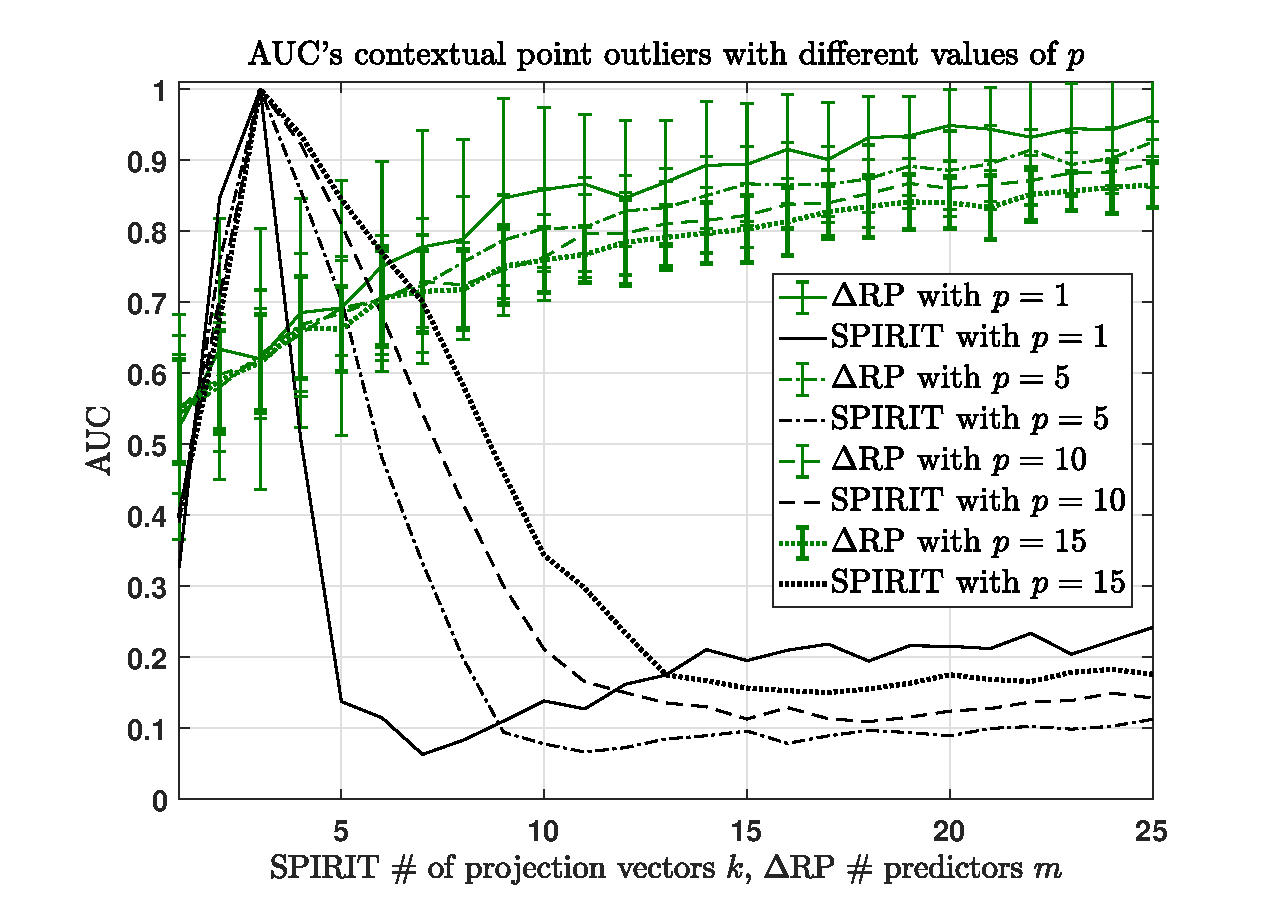
\includegraphics[scale=0.36]{analysis/AUCs_contextual_spiritdelta}
	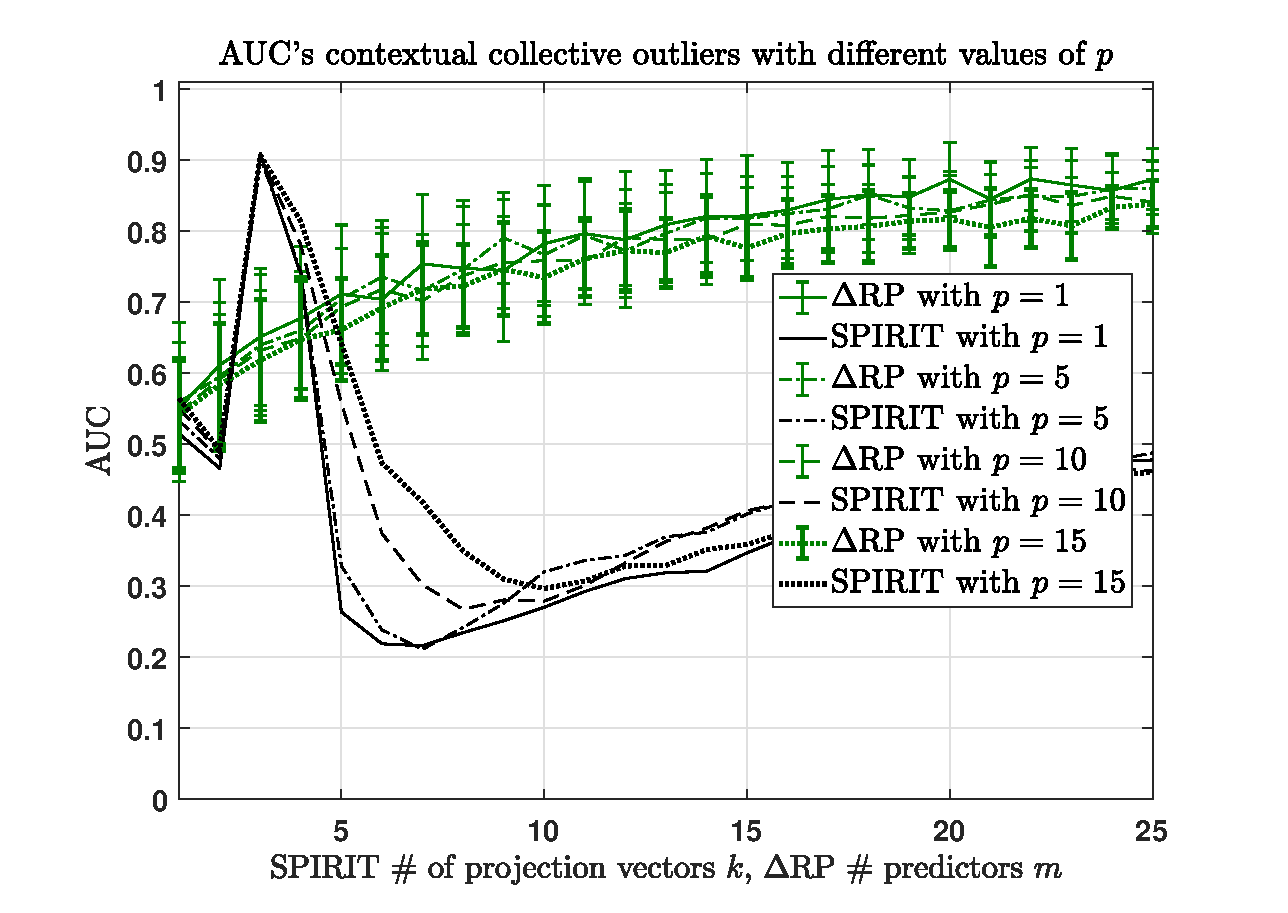
\includegraphics[scale=0.36]{analysis/AUCs_collective_spiritdelta}
	\caption{Detection performances of contextual point and collective outliers with $k$ and $m$ from $1$ to $25$ for $p=\{1,5,10,15\}$.}
	\label{fig:analysis_aucs_contextual_spiritdelta}
	\vspace{-0.05cm}
\end{figure}

We can conclude that the random projection method detects contextual outliers much better when comparing the outlier scores from runs with RP for $k=1$ and $k=2$ than the RP method. Only for the contextual outliers we possibly need a larger set of predictors to approach the optimal performance of SPIRIT. However, it is less sensitive to the number of predictors $m$ than SPIRIT is to the number of projection vectors $k$.


\section{RP and \texorpdfstring{$\Delta$RP}{deltaRP} in online mode}
\label{sec:analysis_worm}

The experiments presented so far led to interesting observations regarding the potential and parameter-sensitivity of the RP method, $\Delta$RP and SPIRIT. In this section, we focus on the online performance of these methods under realistic and fixed parameters. This analysis has also been conducted for standardized data of which the results are presented and discussed in appendix \ref{app:analysis}.

To observe the performance of the methods in online mode, we deploy SPIRIT in its adaptive mode which approximates the number of principal components needed to explain most of the variance online. This requires lower and upper bounds with respect to the explained variance that guide this online adaptation of the number of components. For adaptive SPIRIT, we followed the suggestions from the original paper \cite{papadimitriou2005streaming} for $f_{\hat{E}}$ and $F_{\hat{E}}$. The suggested bounds also resulted in a relatively good detection performance while not being too tight and, therefore, biased towards the data sets. The RP method is deployed with $1$ projection vector, $k=1$, and for $\Delta$RP we present the results for $m=5$ to ensure it has a competitive runtime performance compared to SPIRIT. We did not apply a sliding window such that $p=1$ for all three methods. Table \ref{tab:analysis_parameters} summarizes these parameter settings. 

\begin{table}[h]
	\centering
	\caption{Parameter settings for the analysis in online mode.}
	\label{tab:analysis_parameters}
	\vspace{-0.05cm}
	\begin{tabular}{l c c}
		\toprule	
		\textbf{Method}					& \textbf{Parameter}		& \textbf{Value}		\\
		\midrule
		\multirow{2}{*}{SPIRIT} & $\lambda$				&$	0.97	$	\\
								& $[f_{\hat{E}}, F_{\hat{E}}]$	&	$[0.95, 0.98]$ \\	
		\midrule
		RP				& $k$						&	$1$			\\	
		$\Delta$RP		& $m$						&	$5$			\\	
		\bottomrule		
	\end{tabular}
\end{table}
\vspace{-0.05cm}

Table \ref{tab:analysis_results} shows the results for the methods under these fixed parameter settings for the different types of outliers. The presented results are averaged over $50$ runs with distinct random projection matrices. Bold numbers reflect the on average significantly better performances than the opponent(s) according to the \textit{t}-statistic\footnote{Technically we do not have a standard deviation for SPIRIT as it is a deterministic method, therefore, we took a negligible small standard deviation to compute the \textit{t}-statistic.} \cite{student1908probable}. 

\begin{table}[h]
	\vspace{0.15cm}
	\centering
	\caption{Online performances under fixed parameters.}
	\label{tab:analysis_results}
	\small
	\hspace*{-0.25cm}
	\begin{tabular}{l c c c c c c}
		\toprule	
		\multirow{3}{*}{\textbf{Method}}				&  \multicolumn{2}{c}{\textbf{Global point}}	& \multicolumn{2}{c}{\textbf{Contextual point}} & \multicolumn{2}{c}{\textbf{Contextual collective}}\\	
		\cmidrule{2-7}
						& 	AUC 	& Runtime 	& AUC 	& Runtime 	& AUC 	& Runtime 	\\
		\midrule
		SPIRIT	& $0.79	 $	&$	0.30 (\pm 0.1)	$&$	0.55 $	& $	0.28 (\pm 0.07)$	& 	$	0.58$	& $0.25	(\pm 0.06)$ \\
		
		RP  	& $0.90	(\pm 0.01)$	& $\mathbf{0.01 (\pm 0.00)}$ & $0.28 (\pm 0.01)$	& $\mathbf{0.02 (\pm 0.01)}$	& 	$	0.57 (\pm 0.01)$	& $\mathbf{0.02	(\pm 0.01)}$ \\

		$\Delta$RP		& $\mathbf{0.95 (\pm 0.05)}$	&	$0.21 (\pm 0.06)$	&	$\mathbf{0.71 (\pm 0.16)}$	& 	$0.21 (\pm 0.07)$	&	$\mathbf{0.71 (\pm 0.09)}$		&  $0.22 (\pm 0.04)$	\\
		\bottomrule
	\end{tabular}
\end{table}

From this table it can be concluded that all three methods detect the contextual point outliers worse compared to the global point outliers, while PCA-based models in theory should be less sensitive to such differences. Therefore, it seems likely that this is the consequence of outliers that are actually harder to detect irrespective of the difference in global and contextual outliers. Aside from that, it becomes clear that the default RP method is extremely fast compared to the other methods, while $\Delta$RP significantly improves over SPIRIT regarding the runtime as well. $\Delta$RP outperforms both opponents when it comes to the detection performance regardless of the outlier type.

The resulting balances between the TPR and FPR corresponding to the AUC's in table \ref{tab:analysis_results} are represented by the ROC curves in figure \ref{fig:analysis_rocs_point}. 
It can be seen that $\Delta$RP provides the more desirable operating points for all types of outliers. That is, $\Delta$RP yields on average a better balance between the TPR and FPR for all possible thresholds as based on the outlier scores it generated. However, despite the significantly lower AUC of SPIRIT, it does provide a comparable operating point for global point outliers (left) if an FPR of $0.10$ would be acceptable. The contextual outliers are harder to find for all methods, though $\Delta$RP and SPIRIT do a better job than the RP method. 

\vspace{0.1cm}
\begin{figure}[h]
	\begin{minipage}{0.333\textwidth}
		\centering
		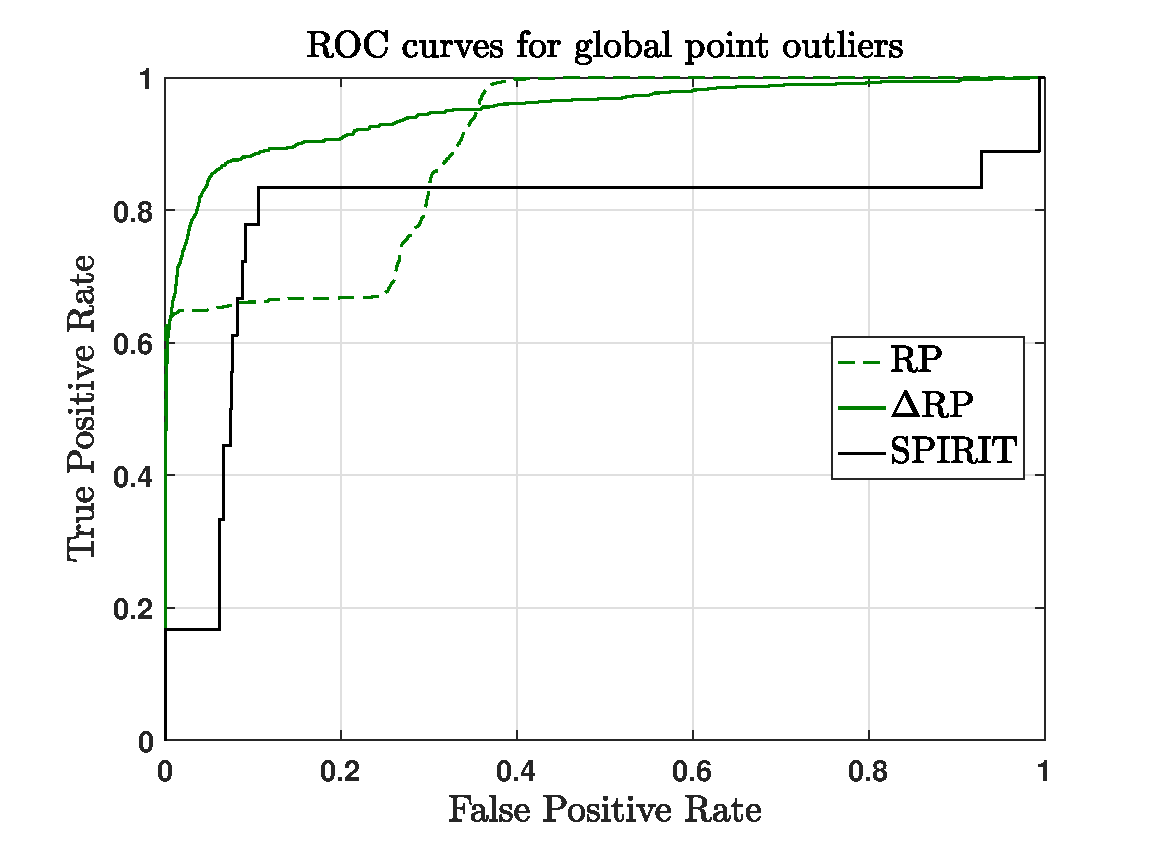
\includegraphics[scale=0.28]{analysis/ROCs_point}
	\end{minipage}
	\begin{minipage}{0.333\textwidth}
		\centering
		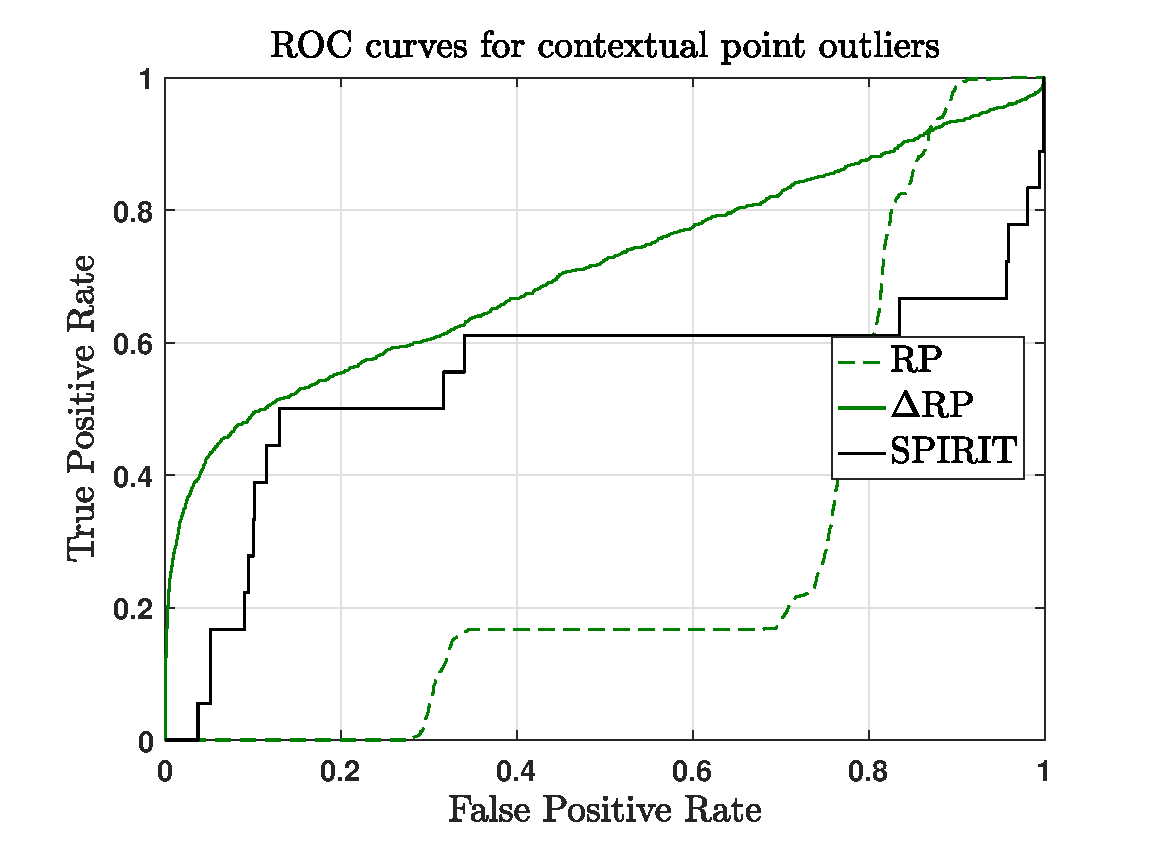
\includegraphics[scale=0.28]{analysis/ROCs_contextual}
	\end{minipage}
	\begin{minipage}{0.333\textwidth}
		\centering
		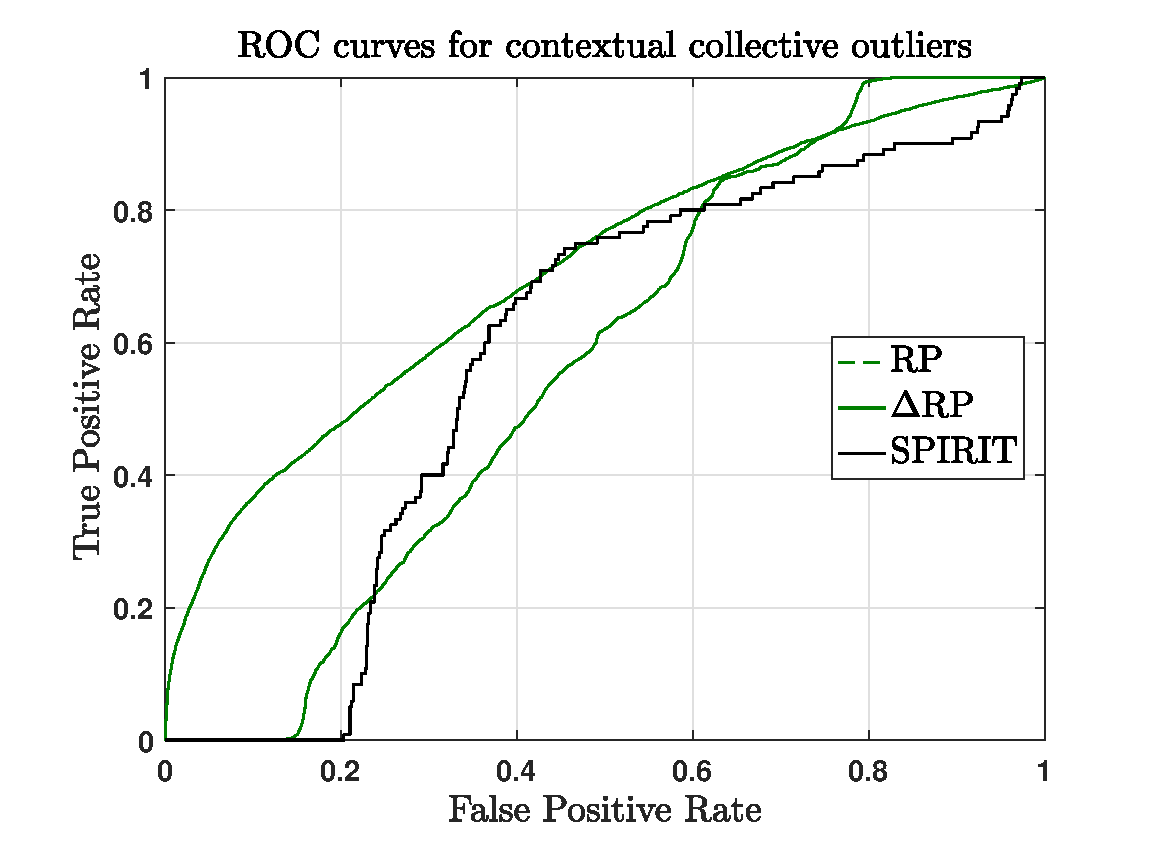
\includegraphics[scale=0.28]{analysis/ROCs_collective}
	\end{minipage}
	\caption{ROC curves of RP, $\Delta$RP and SPIRIT for the three general outlier types.}
	\label{fig:analysis_rocs_point}
\end{figure}


\section{Conclusions}
\label{sec:analysis_concluding}
In this chapter we started with an analysis of the RP method and its performance in the context of unsupervised online outlier detection in multivariate time series. To provide a more thorough understanding of the method, we first showed what actually happens under the hood of the RP method. After gaining these insights we focused, in particular, on the performance in the light of the challenges imposed by our problem context as summarized in table \ref{tab:analysis_evaluation}. To that end, we started with a bird's-eye view of the RP method in comparison to the baseline SPIRIT to determine the effects of the number of projection vectors $k$. As the RP method has difficulties with finding contextual outliers, we adopted a slightly different interpretation (referred to as $\Delta$RP) of the outlier scores which is explained in section \ref{sec:analysis_contextual}. The effectiveness of $\Delta$RP for finding contextual outliers has been evaluated accordingly. Finally, we analysed the performance of the methods when deployed in online mode with fixed parameter settings.

In table \ref{tab:analysis_qualcomp} we provide a qualitative comparison given the evaluation criteria as presented in \ref{tab:intro_characteristics} based on the observations we made in this analysis. We assigned a `$+$' (plus) in case a method was evaluated as best compared to its opponents given a criterion. A `$-$' (minus) is assigned if its performance was not as good as the best method, or a `$/$' (slash) in case the experiments with real-world data are considered necessary to come to a conclusion.

\begin{table}[h]
	\centering
	\vspace{-0.05cm}
	\caption{Evaluation based on the analysis.}
	\label{tab:analysis_qualcomp}
	\begin{tabular}{l c c c}
		\toprule
		\textbf{Evaluation criterion} 		& \textbf{RP} 	& \textbf{$\Delta$RP} & \textbf{SPIRIT} \\ \midrule
		Time needed to process data points 	&  		$+$		&  		$-$		& $-$ \\[0.1cm]
		Dependence on history of stream 	& 		$+$		& 		$+$		& $-$ \\[0.1cm]
		Amount of prior information needed 	& 		$+$		& 		$-$		& $-$ \\[0.1cm]
		Sensitivity of detection performance to parameters 		&	$+$	& 	$-$ 	& $-$ \\
		\midrule
		Generalizability of performances to	different data sets & $/$ & $/$	& $/$ \\[0.1cm]
		Generalizability of performances to different outlier types & $-$	& $+$	& $-$\\
		\midrule
		Influence of $d$ and $n$ on detection performance 		& $/$ & $/$ & $/$ \\[0.1cm]
		Influence of $d$ on runtime	performance	& $+$ & $+$ & $-$ \\
		\bottomrule		
	\end{tabular}
\vspace{-0.1cm}
\end{table}

Starting with the runtime performance, the RP method logically appeared to be significantly faster than $\Delta$RP and SPIRIT. This is mainly because $\Delta$RP runs the RP method $2m$ times, making the default RP method always be the better choice with regard to runtime performance. SPIRIT would be a good choice in case the time series are strongly correlated such that only a few principal coefficient vectors have to be estimated.

Considering the amount of history consumed by a method, adding a sliding window makes SPIRIT its detection performance less sensitive to its parameters. The RP-based methods only benefit a little from a window for contextual outliers. SPIRIT incorporates an additional parameter, forgetting factor $\lambda$, which influences the adaptiveness of the principal coefficient vectors towards the more recent or early history of the data stream. The RP method does not exploit temporal relations by default.

The performance of SPIRIT also relies on the estimated explained variance bounds $f_{\hat{E}}$ (lower) and $F_{\hat{E}}$ (upper), making the number of parameters $2$ in total. Throughout the analysis it turned out that the detection and runtime performances are both sensitive to particularly the variance bounds. This sensitivity also made SPIRIT perform not as good as $\Delta$RP when we analysed the detection performances under fixed parameters in online mode. The default RP method seemed to be parameter-free as it performs best with a single projection vector ($k=1$) for the different outlier types. Increasing the number of projection vectors $k$ for the default RP method only decreases the detection performance a little. $\Delta$RP relies on $1$ parameter, the number of predictors $m$ used to derive an outlier score. Its performance increases smoothly proportionally to the number of predictors $m$ used. The influence of $m$ on the AUC is higher than $k$ for the RP method.

The evaluation regarding the generalizability of the performances of the methods to differently structured data sets is left open as the analysis was conducted with just one data set. We did observe that the detection performance of the methods are sensitive to the mean and range of the data (see appendix \ref{app:analysis}). However, we are also interested in the stability of the performance given different data sets. This is assessed in chapter \ref{chap:experiments}.

We did get a sufficient impression of the generalizability of the methods with respect to the different types of outliers. From the bird's-eye view of the detection performance it became clear that SPIRIT has potential to yield a good AUC for all outlier types. Yet its detection performance suffers from its sensitivity to the parameters. If the analyst has a reasonable understanding of the proper values for the variance bounds to capture the principal behaviour of the time series, SPIRIT might outperform the proposed methods. If the analyst cannot rely on such assumptions, $\Delta$RP will be the better choice, where the default RP method only detects global point outliers well.

Finally, we are also interested in the scalability of the RP-based methods towards high-dimensional data sets. So far, the detection performance of the methods seemed relatively insensitive to the dimensionality of the data. The experiments in chapter \ref{chap:experiments} with differently sized data sets should point out whether the dimensionality has significant impact on the detection performance. When it comes to the runtime performance, we know by the analytical runtime bounds already that the RP-based methods scale better to high $d$ than SPIRIT. That is, the runtime of SPIRIT depends quadratically on $k$ which for SPIRIT is only low if the time series are sufficiently correlated.


\chapter{Experiments}
\label{chap:experiments}

In this chapter we put both analysed methods (RP and $\Delta$RP) at work by detecting outliers in multivariate time series considerably more realistic than synthetically generated from sinusoidal functions. In section \ref{sec:experiments_setup} we discuss the data, performance metrics and parameter settings we used to do so. The results are presented in section \ref{sec:experiments_results}. We also examine the applicability of the RP-based methods on non-temporal data streams by using (non-temporal) data sets commonly used for benchmarking unsupervised (offline) outlier detection methods. The results of these experiments are presented and discussed in section \ref{sec:experiments_beyond}. We conclude this chapter with the key findings and final remarks.

\section{Experimental setup}
\label{sec:experiments_setup}

In chapter \ref{chap:analysis} we already got a good impression of the effectiveness of the methods with regard to the challenges imposed by the task of unsupervised online outlier detection in multivariate time series. Yet two evaluation criteria derived from these challenges were left open by the analysis. First, we want to assess the methods on realistic data and evaluate to what extent their performances depend on the structure of the data. Second, we want to determine the influence of $d$ and $n$ on the detection performance. In this chapter we focus mostly on those two criteria.

\subsection{Data}
To assess the performance of RP, $\Delta$RP and the considered baseline SPIRIT in a real-world context, we used a data set that consists of multiple time series generated by $24$ sensors measuring one water treatment plant (at the same time) \cite{goh2016dataset}. Other data sets commonly used for benchmarking outlier detection in time series such as the Yahoo Web Scope data set \cite{yahoo2015s5} and an outlier-version of the IntelLab data set \cite{bruijn2016benchmark} were not suitable due to the uncorrelated nature of the time series or a limited number of time series, respectively.

The water treatment plant data is originally created for research to cyber attack prevention. Unfortunately, the provided labellings were not aligned with the actual outliers due to a delay between the attack and the actual disruption of the system. Luckily, an attack-free version can be found online as well enabling us to inject the general types of outliers we focused on throughout this thesis ourselves. 

The data set consists of $n=496.800$ data points and $d=24$ time series from sensor readings that measured different parts of the water treatment plant\footnote{The data set also provides actuator readings which were excluded from the data.}. We used the readings of $4$ sensors that measured the same system component, and therefore are sufficiently correlated. We extracted only a fraction of $20.000$ data points from this data set and downsampled the result to a data set of $2.000$ data points.  

The $4$ time series do not have $0$ mean and the ranges of the time series highly differ from each other. As SPIRIT maximizes the variance in the data to derive the principal coefficient vectors, and the reconstructions resulting from random projections are sensitive to the mean of the data, we standardized the data first. This is done by subtracting the mean of each $j^{\text{th}}$ time series ($\mu_j$) from each time series value $\mathbf{x}_{i,j}$ and divide the result by its standard deviation ($\sigma_j$) as in equation \eqref{eq:experiments_normalization}.

\begin{equation}\label{eq:experiments_normalization}
	\tilde{\mathbf{x}}_j = \frac{\mathbf{x}_j - \mu_j}{\sigma_j}
\end{equation}

We injected outliers following similar procedures as in table \ref{tab:analysis_outliers}. However, instead of sampling sequences of $3$ data points we now inject outliers by sequences of $11$ data points. For the global point outliers, we added $3\sigma_j$ to the feature values which should reflect a global outlier \cite{zimek2012survey}. It is hard to actually supervise the `contextualness' of the outliers, therefore we flipped the sign of the data points assuming the resulting values are within the $3\sigma_j$ range from the mean. In figure \ref{fig:experiments_swat} an impression of the $4$ clean time series is given (left), and the result with outliers (right). Note that the actual mean of each time series is $0$ but to avoid occlusion we separated them in this figure. 

\begin{figure}[h]
	\centering
	\includegraphics[scale=0.36]{experiments/Experiments_swat_timeseries}
	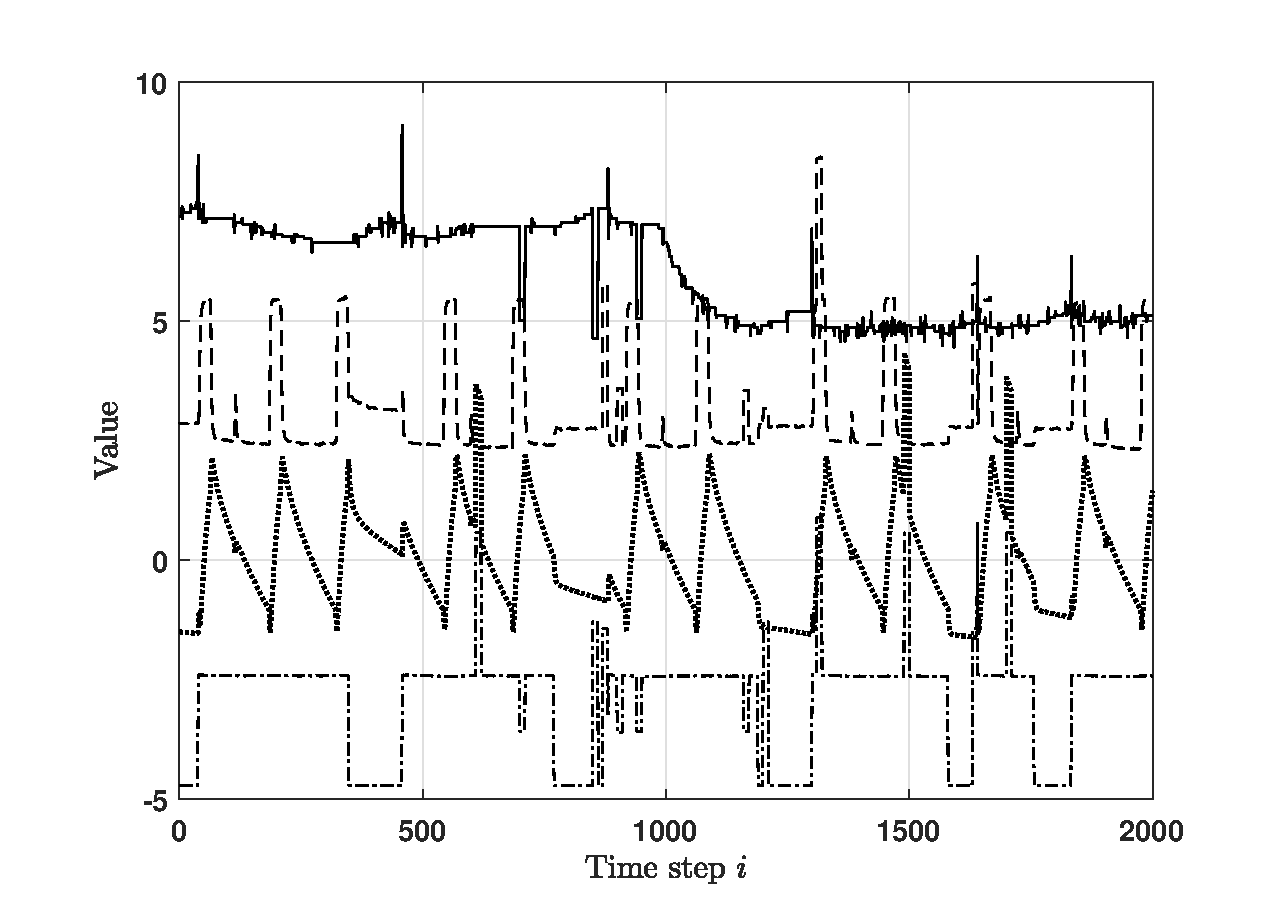
\includegraphics[scale=0.36]{experiments/Experiments_swat_timeseries_outliers}
	\caption{The $4$ time series used from the water treatment plant data set, original (left) and with outliers (right).}
	\vspace{0.2cm}
	\label{fig:experiments_swat}
\end{figure}

Alternatively, a scattermatrix showing all pairwise scatter plots of these $4$ time series can be found in appendix \ref{app:experiments}.

\subsection{Performance metrics and parameters}

For the evaluation on real-world data, we used the same performance metrics as in the previous chapter aside from the number of parameters and preceding data points needed. We left those metrics aside, as we do not focus on criteria of which those metrics are the performance indicators. Besides, the evaluation of the methods with respect to the number of parameters and preceding data points needed are not expected to change much on real-world data. So, we evaluate the method on its detection and runtime performance, with the Area Under the ROC Curve (AUC) and the wall-clock runtime using \texttt{tic} and \texttt{toc} commands in Matlab respectively. 

For $\Delta$RP we kept the parameter $m$ (the number of predictors) low to ensure a low runtime performance. For SPIRIT we slightly explored a range of parameter settings to determine its potential to some extent. However, we kept our exploration of the variance bounds within a sensible range close to the range of $[0.95, 0.98]$ as suggested in \cite{papadimitriou2005streaming}. Table \ref{tab:experiments_parameters} presents the parameter settings used throughout the experiments with real-world data.

\begin{table}[h]
	\centering
	\caption{Parameter settings for the real-world experiments.}
	\label{tab:experiments_parameters}
	\begin{tabular}{l c c}
		\toprule	
		\textbf{Method		}					& \textbf{Parameter			}			& \textbf{Value	}	\\
		\midrule
		\multirow{2}{*}{SPIRIT} 	& $\lambda$						&   $0.97$	\\
										& $[f_{\hat{E}}, F_{\hat{E}}]$	&	$[0.85, 0.95]$ \\
		\midrule
		RP				& $k$							&	$1$			\\	
		$\Delta$RP		& $m$							&	$4$			\\	
		\bottomrule		
	\end{tabular}
\end{table}

\section{Results with water treatment plant data}
\label{sec:experiments_results}

The results of our experiments on the water treatment plant data are presented in table \ref{tab:experiments_results}. The results were averaged over $50$ runs with distinct random projection matrices. Again, results that are significantly better than the opponent(s) according to the \textit{t}-statistic are made bold. 

\begin{table}[h]
	\centering
	\caption{Performances on water treatment plant data.}
	\label{tab:experiments_results}
	\begin{tabular}{l c c }
		\toprule	
		\textbf{Method}		& 	\textbf{AUC }					 	& \textbf{Runtime} 	\\
		\midrule
		SPIRIT		& $0.71$						&  $0.39 (\pm 0.1)$ \\
		RP			& $0.82 (\pm 0.03)$				&  $\mathbf{0.02 (\pm 0.01)}$ \\
		$\Delta$RP	& $\mathbf{0.85 (\pm 0.03)}$	&  $0.31 (\pm 0.06)$ \\
		\bottomrule
	\end{tabular}
\end{table}

For this data, the RP-based methods outperform SPIRIT considering both criteria. The simple RP method with only $1$ projection vector has a significantly better runtime performance as shown in this table. However, it performs little worse in detecting outliers which is caused by its inability of finding contextual outliers. 

As can be seen in figure \ref{fig:experiments_results}, the average ROC curves of the RP method and $\Delta$RP are quite similar. However, if we cannot accept a FPR higher than $0$, the RP method would be a better choice as it yields the highest TPR for FPR $= 0$. If a method is preferred that is able to detect more outliers while minimizing the misclassification costs associated with flagging normal data points as outliers as well, the choice would be the $\Delta$RP method. SPIRIT is probably least desired unless it would be acceptable to incorrectly classify 40\% of the normal data points.

\begin{figure}[h]
	\centering
	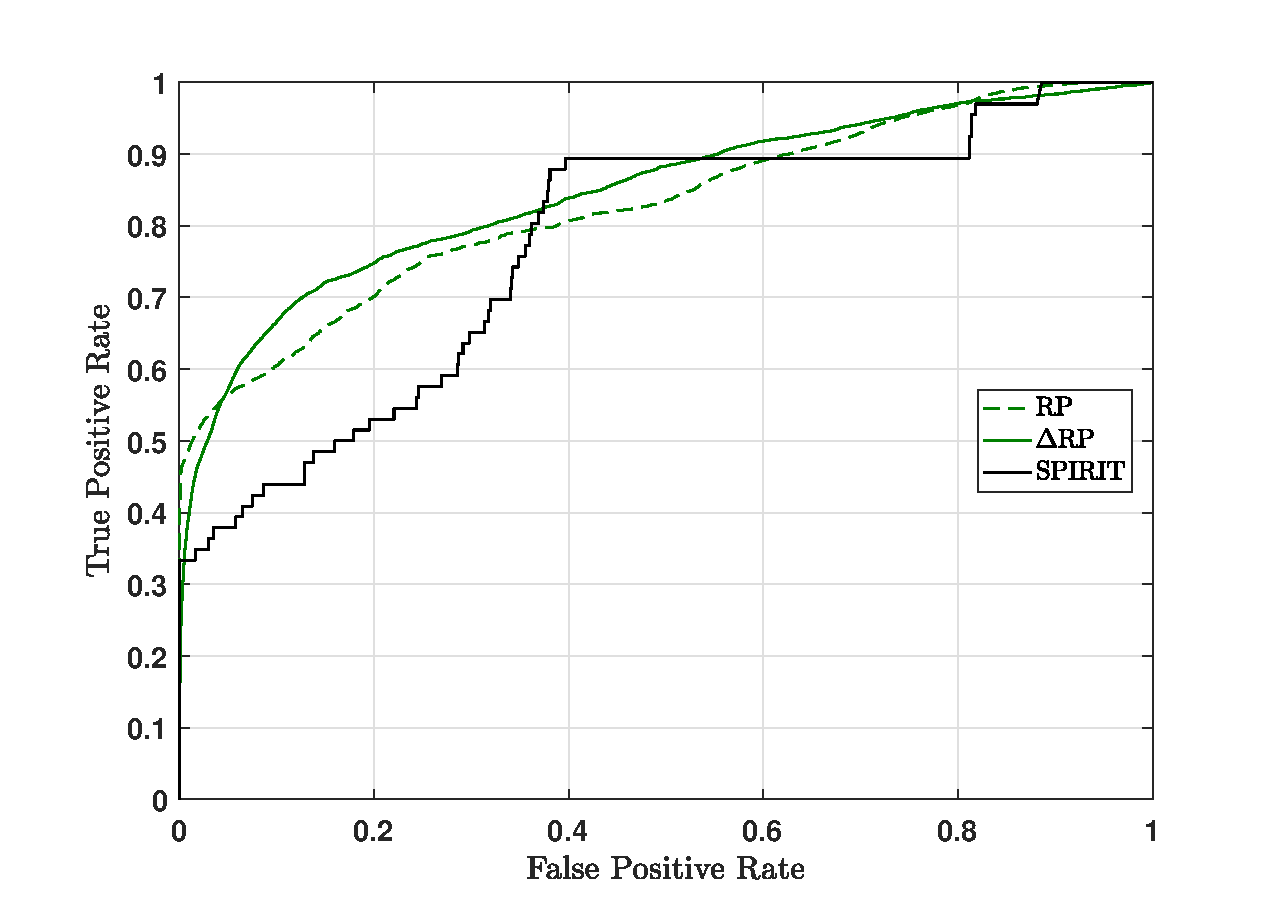
\includegraphics[scale=0.5]{experiments/ROCs_experiments}
	\caption{ROC curves resulting from the experiment with the water treatment plant.}
	\label{fig:experiments_results}
\end{figure}

To shed light on the subtle difference in detection performance of the RP method and $\Delta$RP, we also ran experiments on the same data with only the global or only the contextual outliers. For this experiment, the RP method yields an AUC of $0.99$ for finding the global outliers against $0.98$ for $\Delta$RP and $0.77$ by SPIRIT. However, for the data with only contextual outliers we found an AUC of $0.65$ with the RP method while $\Delta$RP results in an AUC of $0.71$. The AUC obtained by SPIRIT was only $0.36$ explaining its low overall performance of $0.71$. Running PCA offline (when the principal components are learned over the entire data stream) is much better and stable in this case, with an AUC of $0.79$ for global outliers and $0.76$ for contextual outliers. Finally, if we would deploy $\Delta$RP with $m=15$, we can reach an AUC of $0.75$ for the contextual outliers, indicating its unsaturated potential for finding contextual outliers.


\section{Results with non-temporal benchmark data}
\label{sec:experiments_beyond}

As a consequence of the conclusions that the proposed RP-based methods do not exploit temporal relations within time series, and suitable temporal data sets are rarely available online, we also compared our method on non-temporal data sets. Plenty of data sets frequently used for benchmarking unsupervised outlier detection methods are available, which also have more features than our water treatment plant data. As this task does not require an online method we left the online mean and variance estimation aside and deploy $\Delta$RP offline but still unsupervised. This also means that we can compare our method with methods that are not limited to online outlier detection such as the well-known Local Outlier Factor (LOF) which is based on density estimation \cite{breunig2000lof} and offline PCA.

We used $6$ data sets of which the characteristics are described in table \ref{tab:experiments_beyond_data}. These data sets can be retrieved from the UCI Machine Learning repository \cite{uci2018data} as well as the Outlier Detection Dataset repository of Stony Brook University \cite{odds2016}. The data sets used for these experiments all have a clear notion of what is considered normal and abnormal, e.g. data points correspond to healthy persons or persons suffering from a disease (for instance breast cancer or diabetes). 

\begin{table}[h]
	\centering
	\vspace{-0.05cm}
	\caption{Non-temporal benchmark data sets for unsupervised outlier detection.}
	\label{tab:experiments_beyond_data}
	\begin{tabular}{l c c c}
		\toprule	
		\textbf{Method}		& 	\textbf{$\#$ data points $n$}	& \textbf{$\#$ features $d$} & \textbf{$\#$ outliers}	\\
		\midrule
		Mammography	& $11,183$	&   $6$		&	$260 \ (2.3 \%)$	\\
		Thyroid (Ann-)	& $6,832$	&   $6$		&	$534 \ (7.4 \%)$	\\
		Pima		& $768$		&   $8$		& 	$268 \ (35 \%)$	\\
		Breast Cancer Wisconsin (BCW)	& $683$		& 	$9$		&	$239 \ (35 \%)$	\\
		Arrhythmia	& $452$		&	$274$	&	$66 \ (15\%)$		\\
		Ionosphere	& $351$		&	$32$	&	$126 \ (36\%)$	\\
		\bottomrule
	\end{tabular}
	\vspace{-0.05cm}
\end{table}

For the standard RP method we used only one projection vector, i.e. $k=1$, which was observed to yield the best performance. For $\Delta$RP we have set the number of predictors $m$ to $15$ as we are not concerned with optimizing the runtime performance since we compare the performances offline.
The results corresponding to the LOF method were extracted from \cite{liu2008isolation}. They deployed the density-based LOF method with a commonly used parameter $k=10$ reflecting the number of neighbours used in defining the local neighbourhood of each data point. We explored the performance of offline PCA with several variance bounds on all data sets in table \ref{tab:experiments_beyond_data} and set its parameter to a sensible value of $90\%$. For the reconstruction-based methods (RP, $\Delta$RP and PCA) we standardized the data following equation \eqref{eq:experiments_normalization} where we excluded features $j$ of $d$ that have $\sigma_j = 0$.

Table \ref{tab:experiments_beyond} shows the results of this experiment which were averaged over $50$ runs with distinct random projection matrices. Bold scores correspond to the significantly best performance according to the \textit{t}-statistic. The detection performance of the RP method and $\Delta$RP on unstandardized data can be found in appendix \ref{app:experiments}. 

\begin{table}[h]
	\centering
	\vspace{-0.05cm}
	\caption{Detection performances on \textit{standardized} non-temporal data sets.}
	\label{tab:experiments_beyond}
	\begin{tabular}{l c c c c}
		\toprule	
		\multirow{2}{*}{\textbf{Dataset}} & \multicolumn{4}{c}{\textbf{AUC}} \\
		\cmidrule{2-5}
					& \textbf{RP} 						& \textbf{$\Delta$RP} 			&  \textbf{PCA}		& \textbf{LOF}	\\
		\midrule
		Mammography & $\mathbf{0.88 (\pm 0.02)}$		& $\mathbf{0.88 (\pm 0.01)}$	& $0.76$			& $0.67$  	\\
		Thyroid (Ann-)  & $0.67 (\pm 0.00)$ 				& $0.64 (\pm 0.02)$ 			& $0.49$			& $\mathbf{0.72}$	\\
		Pima 		& $\mathbf{0.65 (\pm 0.01)}$ 		& $\mathbf{0.65 (\pm 0.01)}$ 	& $0.57$			& $0.49$	\\	
		BCW  	& $0.95 (\pm 0.01)$					& $\mathbf{0.97 (\pm 0.01)}$ 	& $0.89$			& $0.37$	\\
		Arrhythmia	& $\mathbf{0.77 (\pm 0.00)}$ 		& $0.75 (\pm 0.02)$  			& $0.63$			& $0.73$	\\
		Ionosphere	& $0.79 (\pm 0.00)$ 				& $0.80 (\pm 0.02)$  			& $\mathbf{0.95}$	& $0.89$	\\
		\bottomrule
	\end{tabular}
	\vspace{-0.05cm}
\end{table}

Clearly, the RP-based methods give a quite stable performance considering all data sets, as most AUC's are quite close to the AUC of the best scoring method on a given data set. Only for the Ionosphere data set, the proposed methods perform much worse than PCA and LOF. Overall seen, the RP method and $\Delta$RP are quite comparable in detection performance. Yet the experiments with the unstandardized data point out that the RP method is more sensitive to standardization than $\Delta$RP. 

\section{Conclusions}
In this chapter we exposed the methods to real-world data sets. We examined the methods on (semi-realistic) temporal data for which they were intended. However, we also examined the generalizability of the methods to non-temporal data streams. The reasons for doing so, is that our method actually does not exploit any temporal relations and there is a lack of temporal data sets available that suited our conditions. The main objective of the experiments was to evaluate the methods with regard to the two criteria still open after the analysis. In table \ref{tab:experiments_qualcomp} we provide our conclusions with respect to those two criteria. 
We assigned a `$+$' (plus) in case a method was evaluated as best compared to its opponents given a criterion, or a `$-$' (minus) if its performance was not as good as the best method.

\begin{table}[h]
	\centering
	\vspace{0.1cm}
	\caption{Evaluation based on the experiments.}
	\label{tab:experiments_qualcomp}
	\begin{tabular}{l c c c}
		\toprule
		\textbf{Evaluation criterion} 		& \textbf{RP} 	& \textbf{$\Delta$RP} & \textbf{SPIRIT} \\ \midrule
		Generalizability of performances to different data sets  & $-$ & $+$	& $-$ \\[0.15cm]
		Influence of $d$ and $n$ on	detection performance & $+$ & $+$ & $+$ \\
		\bottomrule		
	\end{tabular}
	\vspace{0.1cm}
\end{table}
 
As observed throughout the analysis and experiments, SPIRIT and the RP method are more sensitive to the mean and range of the data than $\Delta$RP. When it comes to most non-temporal data sets, both RP-based methods outperform a well-known unsupervised outlier detection method based on the Local Outlier Factor and offline PCA. For $4/6$ non-temporal outlier detection benchmark data sets an RP-based method performs better.
In general, $\Delta$RP has shown to yield the most stable performance on synthetic, semi-realistic and real-world data, on temporal and non-temporal, standardized and unstandardized data sets (appendix \ref{app:experiments}).

We could not derive a clear correlation between the detection performance and the dimensionality of the data from the analysis in chapter \ref{chap:analysis} and the experiments in this chapter. Therefore, it seems that the analysed methods are relatively insensitive to the dimensionality of the data. The main problem as identified in section \ref{sec:introduction_complexity}, is that the difference between outlier scores might vanish when $d$ and/or $n$ become large \cite{beyer1999nearest}. But Zimek et al. \cite{zimek2012survey} already found that the dimensionality might not significantly affect outlier detection methods that compute outlier scores based on the Euclidean distance. This statement might hold for methods that compute outlier scores from the squared Euclidean distance as well. Therefore we also ran some small experiments with taking the squared Euclidean norm of each data point directly as outlier score. This measure appeared to be very effective for global outliers, but does not work for contextual outliers. Yet if one wants to find global outliers in extremely high-dimensional data sets, the squared Euclidean distance seems already relatively insensitive to the curse of dimensionality.



\chapter{Conclusion}
\label{chap:discussion}

In this chapter we recapitulate what has been discussed in this thesis by means of a summary in section \ref{sec:discussion_summary}. What we conclude from this thesis with respect to the initial research question is discussed in section \ref{sec:discussion_conclusions}. Finally, we provide future research directions in section \ref{sec:discussion_future} by identifying limitations of the proposed methods and conducted research, and highlighting the remaining open questions.

\section{Summary}
\label{sec:discussion_summary}

In this thesis we considered the task of unsupervised online outlier detection in multivariate time series. The difficulties imposed by this task as introduced in chapter \ref{chap:introduction} can be summarized as follows.

\begin{itemize}
	\itemsep-0.2em
	\item The algorithm should be minimally sensitive to its parameters, require limited prior information, and label each data point before the next point is received.	
	\item The analyst should have an idea of the structure of the data and expected outliers.
	\item The algorithm should be able to detect global as well as contextual outliers in time series.
	\item The algorithm has to scale well to high-dimensional data sets, with respect to its computational complexity and its detection performance despite the curse of dimensionality.
\end{itemize} 

These challenges motivated us to concentrate our research around the question: \textit{can we leverage random projections in an online and unsupervised reconstruction-based method in order to find outliers in multivariate time series effectively though more efficiently, and if so, to what extent?} To that end, in chapter \ref{chap:reconstruction-detection} we first explained the theory behind reconstruction-based methods. We also discussed a well-known online method called SPIRIT which is based on approximate principal component analysis. This method has been adopted as a baseline method for comparison purposes. 

We continued with an explanation of the proposed random projection method (RP), and finally presented its entire procedure by means of algorithm \ref{alg:analysis_algorithm} in chapter \ref{chap:rp-method}. Its procedure basically revolves around a projection of the time series into a lower-dimensional random subspace, from which the reconstruction is used as model of the data. Hopefully, an outlier is then poorly reconstructed such that the squared Euclidean distance between the original data point and its reconstruction results in a higher outlier score than for normal data points.
Throughout the analysis with the RP method in chapter \ref{chap:analysis}, we found that it finds global point outliers very accurately and efficiently. And as opposed to SPIRIT, it is relatively insensitive to its parameters. However, we also showed that it is not successful in finding contextual outliers, which is certainly an undesired conclusion.

Fortunately, we discovered that the RP method often works better when it projects the data into a $1$-dimensional subspace instead of a ($1+\Delta$)-dimensional subspace with $\Delta > 0$. This implies that a reconstruction from a $1$D projection, on average, results in a more discriminative outlier measure than a reconstruction from a $2$D projection. This resulted in formulating hypothesis \ref{hyp:analysis_outlierinlier} which directly led us to a different interpretation of the outlier scores of the RP method. This alternative interpretation resulted in a method we call $\Delta$RP which basically runs the RP method twice: once with $1$ projection vector and once with $2$ vectors. The standardized difference between the two resulting outlier scores is then interpreted as the final outlier score. This outlier measure appeared to be more effective for finding outliers in general, though increases the computational burden compared to the default RP method as more than $1$ predictions for the outlier score are needed to obtain a reliable outlier score.

The experiments with real-world data in chapter \ref{chap:experiments} showed that for realistic data structures, $\Delta$RP is significantly faster than its baseline SPIRIT without the loss of detection performance. It was also shown that the RP method yields, on average, a good detection performance and is evidently the fastest method. Yet it comes with the cost of misclassifying a larger fraction of contextual outliers compared to $\Delta$RP.
The latter appears to be relatively insensitive to the number of predictors $m$, which basically proportionally improves the certainty and accuracy of the predictions. SPIRIT needed some exploration of its parameter settings beforehand to find a proper operating point as its performance is highly sensitive to the parameters.
Finally, we assessed the RP-based methods on non-temporal data for which the proposed methods appeared to be successfully applicable too.


\section{Conclusions}
\label{sec:discussion_conclusions}

In chapter \ref{chap:introduction} we identified the primary challenges imposed by our problem context which we translated to a set of evaluation criteria in section \ref{sec:analysis_methodology}. In table \ref{tab:conclusion_qualcomp} we combine the observations from the analysis and experiments into a final evaluation of the proposed methods in comparison with SPIRIT. For each criterion we determined which method is evaluated best and assigned a `$+$' (plus) to that method. We assigned a `$-$' (minus) to the methods that perform worse on the given criterion. 

\begin{table}[h]
	\centering
	\vspace{0.05cm}
	\caption{Final evaluation of the proposed methods against the baseline.}
	\label{tab:conclusion_qualcomp}
	\begin{tabular}{l c c c}
		\toprule
		\textbf{Evaluation criterion} 		& \textbf{RP} 	& \textbf{$\Delta$RP} & \textbf{SPIRIT} \\ \midrule
		Time needed to process data points 	&  		$+$		&  		$-$		& $-$ \\[0.12cm]
		Dependence on history of stream 	& 		$+$		& 		$+$		& $-$ \\[0.12cm]
		Amount of prior information needed 	& 		$+$		& 		$-$		& $-$ \\[0.12cm]
		Sensitivity of detection performance to parameters			&	$+$ 	& 	$-$	& $-$ \\
		\midrule
		Generalizability of performances to different data sets & $-$ & $+$ & $-$\\[0.12cm]
		Generalizability of performances to different outlier types	& $-$	& $+$	& $-$\\
		\midrule
		Influence of $d$ and $n$ on detection performance		& $+$ & $+$ & $+$ \\[0.12cm]
		Influence of $d$ on runtime performance		& $+$ & $+$ & $-$ \\
		\bottomrule		
	\end{tabular}
	\vspace{0.05cm}
\end{table}

Considering the runtime performance of the methods analysed in this thesis, the RP method as formulated in algorithm \ref{alg:analysis_algorithm} was evidently the most efficient. Aside from that, it does not generalize well to all types of outliers and data sets. $\Delta$RP would therefore be a safe second choice when it comes to runtime and detection performance. 

When it comes to the dependency on the history of a data stream, none of the RP-based methods exploit correlations between data points over time. Both methods solely rely on the correlation among the different time series. SPIRIT does track temporal relations which is incorporated internally by a so-called forgetting factor. Still, SPIRIT benefits from a sliding window as its detection performance becomes less sensitive to its initial parameters. Altogether, the RP-based methods are considered preferable with respect to their (in)dependence of the history of a data stream.

Throughout the analysis and experiments it became clear that the RP method performs best if we deploy it with only $1$ projection vector. Therefore, the RP method could be regarded as a parameter-free method, requiring no prior information to set its only parameter: the number of projection vectors $k$. It also turned out to be the least sensitive to this parameter, explaining its positive evaluation with respect to the sensitivity of the detection performance. 

The analysis and experiments pointed out that $\Delta$RP generalizes very well to all different data sets we used. This is a very desirable property making this method suitable for a broad range of applications. $\Delta$RP is also the best choice when it comes to finding all outliers of the considered types: global point outliers, contextual point outliers and contextual collective outliers. That said, $\Delta$RP is considered the most generally applicable method with respect to the structure of the data, and the outlier types that can possibly be found.

The final two criteria relate to the influence of the dimensionality of the data stream. First, we should be able to find significantly outlying data points in a very large set of $n$ data points. Second, this should also be possible for an increasing dimensionality $d$ of each data point. Though methods might not be able to do so, we found that reconstruction-based methods in general do not suffer from this problem. At least, we did not find sufficient evidence of a correlation between the dimensionality of the data and the detection performance of a method. This observation corresponds to the statement of Zimek et al. \cite{zimek2012survey} that in particular outlier detection methods computing outlier scores based on Euclidean distances not necessarily suffer from the curse of dimensionality. Still, the number of time series does influence the runtime of SPIRIT more than RP-based methods, in a negative sense. This is caused by the potentially increasing number of principal components $k$ needed to estimate when the number of time series is high, where the runtime of SPIRIT depends quadratically on $k$.
 
Returning to our research question: we presented two effective and efficient methods that exploit the reconstruction error from random projections to derive outlier scores in an online and unsupervised manner. Besides, both RP-based methods are relatively insensitive to the parameters as opposed to most online outlier detection methods. Yet the most efficient method (RP) is not generally applicable as it lacks the ability to find contextual outliers, which is considered very important for outlier detection methods. The method proposed to resolve this problem ($\Delta$RP) is less efficient but generalizes well to different outlier types and data sets. Still, $\Delta$RP is in most cases more efficient than SPIRIT. If we make up the balance given the identified challenges, $\Delta$RP would be the overall best choice.


\section{Future work}
\label{sec:discussion_future}

From this thesis we already got a fair impression of the potential of the proposed methods. Still, we are left with some open questions interesting to answer in the future. Starting with the limitations of this research we think it would be interesting to experimentally assess the applicability of the methods on more differently structured (temporal) data sets with varying outlier densities. Additionally, we did not find enough evidence of a correlation between the detection performances and the number of time series $d$ or data points $n$, which seems valuable to study further. 

Furthermore, we did not explore the influence of the strength of the correlations between the time series, yet this correlation is an important condition for the RP-based methods to work well. Finally, we focused on comparing our methods to an established method which functioned as a baseline. Evaluating the performance of the methods against more recently introduced methods (e.g. Loda \cite{pevny2016loda} as discussed in section \ref{sec:introduction_related}) would be valuable.

We also identified some limitations of the proposed methods RP and $\Delta$RP, which are interesting to look at in the future. Throughout the analysis, we concluded that both methods do not significantly benefit from a window, nor track any temporal relations internally. Especially the default RP method could benefit from doing so, as in its current formulation it does not detect the contextual outliers well. 

The method we propose to find contextual outliers better, $\Delta$RP, relies on the assumption that outliers are reconstructed relatively better compared to normal data points when the number of projection vectors is increased. However, the random factor associated with the data projections introduces a significant uncertainty of the detection performance, which can be compensated by increasing the number of predictors $m$. For future research, it would be valuable to explore heuristics that would result in an accurate a priori setting for $m$. This would make it easier to settle on the desired balance between the detection and runtime performances before $\Delta$RP is deployed.

Nevertheless, the most pressing question that is left unanswered is whether hypothesis \ref{hyp:analysis_outlierinlier} can be proven formally. If so, it opens a few additional questions we would be interested in:
\begin{itemize}
	\item What is the probability associated with this hypothesis such that it holds on expectation?
	\item What technicality stands at the basis of this probability, i.e. what property of the data or the random projection matrices makes it stand or fall?
\end{itemize}

In general, we encourage theoretical analysis to prove hypothesis \ref{hyp:analysis_outlierinlier}. Finally we only explored the RP-based methods with Gaussian dense random matrices. Though, a significant body of research has been devoted to advancing the random projection matrices with respect to the runtime performance. It might be interesting to discover the effects of the different variants out there, as in this thesis we only explored the tip of the iceberg.


\chapter*{Acknowledgements}
\addcontentsline{toc}{chapter}{Acknowledgements}
\label{chap:acknowledgements}

\bigskip

First and foremost I would like to express my gratitude to my supervisor David Tax, without whose constant advice and challenging attitude this thesis would not be here. A special thanks goes to my family, who supported every decision along the road and made my route possible in the first place. Nonetheless, I cannot thank Lute enough as without him, my time as a student at the faculty of EEMCS would have been much less smooth, pleasant and successful. Finally, I am thankful for the stimulating discussions and collaborations with fellow students over the past few years, and for the enjoyable time I had in Delft with people that became close friends.

\bibliography{report-bib}

\appendix
\chapter{Additional analysis results}
\label{app:analysis}

In this appendix we present results of the analysis that were left out of the body of the thesis. First we present the analysis of the effect of different window lengths $p$ ($1,5,10$ and $15$) on the detection performance in section \ref{sec:app_windowsizes}. In section \ref{sec:app_rp_standardized} we present the results corresponding to the analysis on the standardized data with the RP method and $\Delta$RP in comparison with baseline SPIRIT.

\section{Detection performance of RP with different window sizes}
\label{sec:app_windowsizes}
Throughout the body of this thesis we found that using a sliding window did not significantly improve the RP method nor the considered baseline SPIRIT. This is a logical observation for the RP method which does not take the temporal relations into account, but merely relies on the correlation among the different time series. For SPIRIT though, one might expect that it benefits from a sliding window. However, this specific method already incorporates a forgetting factor $\lambda$ that relates to the influence of the most recent part of the stream against its early history as explained in chapter \ref{chap:reconstruction-detection}. Still, the performance of SPIRIT is slightly affected by a sliding window since the forgetting factor is only a suboptimal solution to learn temporal relations to improve runtime performance. 

For the synthetic data set we used throughout the analysis, adding a sliding window mainly improves the detection performance of SPIRIT regarding the sensitivity to the number of projection vectors $k$. Logically, the runtime performance is much worse when we add a window. The effect of the number of projection vectors $k$ on the runtime is, however, very similar to what was already shown in figure \ref{fig:analysis_runtimes_point} in chapter \ref{chap:analysis}. Therefore, we do not present the runtime performances for different values of $p$.
Figure \ref{fig:app_aucs_point} shows the detection performances for global point outliers for the different window sizes. These results are presented and discussed in section \ref{sec:analysis_bird}, but were included for the sake of completeness.

\begin{figure}[h]
	\centering
	\includegraphics[scale=0.36]{analysis/AUCs_point}
	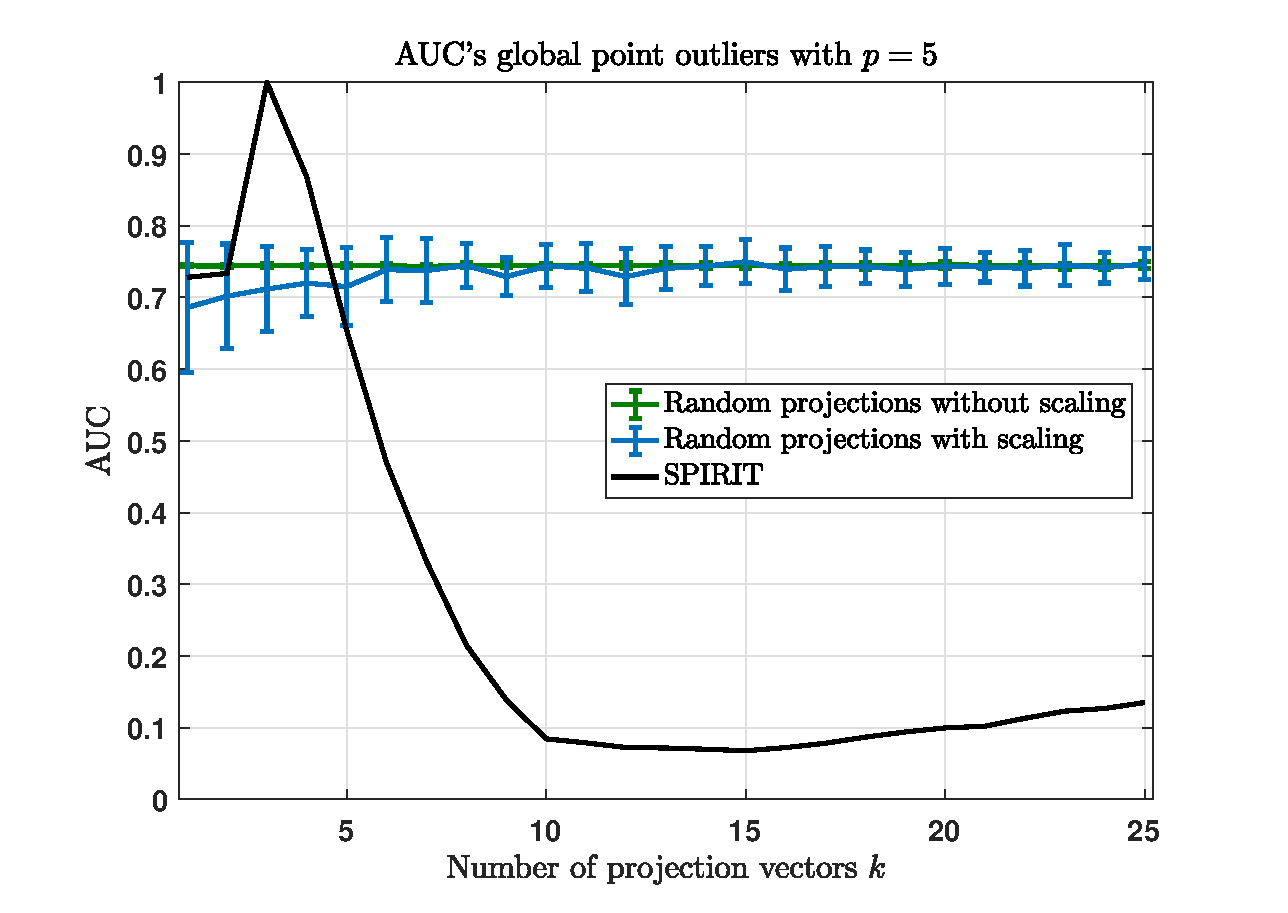
\includegraphics[scale=0.36]{analysis/AUCs_point1}
	\phantomcaption
	\label{fig:app_aucs_point}
\end{figure}%
\begin{figure}[h]\ContinuedFloat
	\centering
	\includegraphics[scale=0.36]{analysis/AUCs_point2}
	\includegraphics[scale=0.36]{analysis/AUCs_point3}
	\caption{Detection performances of global point outliers with $k$ from $1$ to $25$ for $p=\{1,5,10,15\}$.}
	\label{fig:app_aucs_point}
\end{figure}

\newpage
Figure \ref{fig:app_aucs_contextual} shows the performances corresponding to the detection of contextual point outliers. The only difference we observe here as a consequence of varying $p$ besides the poor performance in general, is that the AUC of the RP method improves a little when we adopt a sliding window.

\begin{figure}[h]
	\centering
	\includegraphics[scale=0.36]{analysis/AUCs_contextual}
	\includegraphics[scale=0.36]{analysis/AUCs_contextual1}
	\includegraphics[scale=0.36]{analysis/AUCs_contextual2}
	\includegraphics[scale=0.36]{analysis/AUCs_contextual3}
	\caption{Detection performances of contextual point outliers with $k$ from $1$ to $25$ for $p=\{1,5,10,15\}$.}
	\label{fig:app_aucs_contextual}
\end{figure}

Figure \ref{fig:app_aucs_collective} shows the performances corresponding to the detection of contextual collective outliers. Again, besides the poor performance, the main difference in behaviour is that the AUC of the RP method is slightly improved when adopting a sliding window.

\begin{figure}[h]
	\centering
	\includegraphics[scale=0.36]{analysis/AUCs_collective}
	\includegraphics[scale=0.36]{analysis/AUCs_collective1}
	\includegraphics[scale=0.36]{analysis/AUCs_collective2}
	\includegraphics[scale=0.36]{analysis/AUCs_collective3}
	\caption{Detection performances of contextual collective outliers with $k$ from $1$ to $25$ for $p=\{1,5,10,15\}$.}
	\label{fig:app_aucs_collective}
\end{figure}

\newpage
\section{RP and \texorpdfstring{$\Delta$RP}{deltaRP} on standardized data}
\label{sec:app_rp_standardized}
In this section we present the results of the RP method in comparison to SPIRIT for the (offline) standardized versions of the synthetic data sets used in chapter \ref{chap:analysis}. We standardized the data set $\mathbf{X}$ by subtracting the mean of each $j^{\text{th}}$ time series ($\mu_j$) from each time series value $\mathbf{x}_{i,j}$ and divide the result by its standard deviation ($\sigma_j$) as in equation \eqref{eq:app_analysis_normalization}.

\begin{equation}\label{eq:app_analysis_normalization}
	\tilde{\mathbf{x}}_j = \frac{\mathbf{x}_j - \mu_j}{\sigma_j}
\end{equation}

As the behavioural observations of the performances with different window sizes are not significantly different from unstandardized data, we only present the results of the methods without a sliding window (i.e. $p=1$). The runtime of the RP-based methods is completely insensitive to the mean and range of the data, where the runtime of SPIRIT is also not affected significantly. Therefore, we did not include the runtime performances associated with the standardized data sets. 

Starting with the bird's-eye view of the RP method for standardized data, figure \ref{fig:app_aucs_standardized} shows the results for the number of projection vectors $k$ ranging from $1$ to $25$. 

\vspace{-0.25cm}
\hspace{-0.15cm}
\begin{figure}[h]
	\hspace{-0.2cm}
	\begin{minipage}{0.333\textwidth}
		\centering
		\includegraphics[scale=0.26]{analysis/AUCs_point_standardized}
	\end{minipage}
	\begin{minipage}{0.333\textwidth}
		\centering
		\includegraphics[scale=0.26]{analysis/AUCs_contextual_standardized}
	\end{minipage}
	\begin{minipage}{0.333\textwidth}
		\centering
		\includegraphics[scale=0.26]{analysis/AUCs_collective_standardized}
	\end{minipage}
	\caption{Detection performances of all three outlier types, with standardized data with $k$ from $1$ to $25$ for $p=1$.}
	\label{fig:app_aucs_standardized}
	\vspace{-0.2cm}
\end{figure}

For global point outliers (figure \ref{fig:app_aucs_standardized}, left), SPIRIT already reached an AUC of $1$ on unstandardized data and therefore no significant overall improvement can be detected. However, SPIRIT now has $3$ parameter settings ($k=1,2,3$) such that the AUC is above $0.80$. For the RP method we can clearly see that the performance is much better when the data is standardized as the RP method without back-scaling attains an AUC of $1$ irrespective of the number of projection vectors $k$, where its version with back-scaling approaches $1$ as well for sufficient $k$. Indeed, we can conclude that the RP method is not sensitive to $k$ in order to find global point outliers.

For contextual point outliers (figure \ref{fig:app_aucs_standardized}, center), especially SPIRIT improves regarding the AUC which now is close to $1$ for a larger range of the number of projection vectors $k$. That said, the RP method does not benefit from standardized data for finding contextual point outliers. A remarkable difference in the detection performances can be derived with respect to the contextual collective outliers (figure \ref{fig:app_aucs_standardized}, right). The RP method and baseline SPIRIT both perform worse for finding contextual collective outliers. While the RP methods (with and without back-scaling) obtained stable AUC's around $0.6$ and SPIRIT (at most) $0.9$, both optimal performances drop to $0.45$ and $0.73$, respectively.\\

Figure \ref{fig:app_aucs_spiritdelta_standardized} shows the detection performances of $\Delta$RP for different numbers of predictors $m$ in comparison with SPIRIT with different values for $k$. 

\hspace{-0.15cm}
\vspace{-0.2cm}
\begin{figure}[h]
	\hspace{-0.2cm}
	\begin{minipage}{0.333\textwidth}
		\centering
		\includegraphics[scale=0.26]{analysis/AUCs_point_spiritdelta_standardized}
	\end{minipage}
	\begin{minipage}{0.333\textwidth}
		\centering
		\includegraphics[scale=0.26]{analysis/AUCs_contextual_spiritdelta_standardized}
	\end{minipage}
	\begin{minipage}{0.333\textwidth}
		\centering
		\includegraphics[scale=0.26]{analysis/AUCs_collective_spiritdelta_standardized}
	\end{minipage}
	\caption{Detection performances of all three outlier types, with standardized data with $k$ and $m$ from $1$ to $25$ for $p=1$.}
	\label{fig:app_aucs_spiritdelta_standardized}
	\vspace{0.1cm}
\end{figure}

Similar to the RP method, $\Delta$RP finds global point outliers (left) very accurately, approaching an AUC of $1$. In contrast to the RP method, however, it also successfully detects most contextual point outliers as well (center). Besides, it reaches an acceptable AUC with slightly less predictors than when the data is not standardized. For example, to obtain an AUC of approximately $0.90$ $\Delta$RP requires around $15$ predictors ($m=15$) when the data is not standardized. If standardization is possible, it attains an AUC of $0.90$ with around $12$ predictors ($m=12$). When it comes to the detection performance regarding contextual collective outliers (right), a similar observation can be made as for the RP method and SPIRIT. That is, finding contextual collective outliers apparently is harder when the data is standardized.

We also present the results of the methods when they are deployed in online mode on the standardized data. We used the same parameter settings as in table \ref{tab:analysis_parameters} which are presented again in table \ref{tab:app_analysis_parameters}. 

\begin{table}[h]
	\centering
	\vspace{0.05cm}
	\caption{Parameter settings for the analysis in online mode.}
	\label{tab:app_analysis_parameters}
	\begin{tabular}{l c c}
		\toprule
		\textbf{Method}					& \textbf{Parameter}		& \textbf{Value}		\\
		\midrule
		\multirow{2}{*}{SPIRIT} & $\lambda$				&$	0.97	$	\\
		& $[f_{\hat{E}}, F_{\hat{E}}]$	&	$[0.95, 0.98]$ \\
		\midrule
		RP				& $k$						&	$1$			\\
		$\Delta$RP		& $m$						&	$5$			\\
		\bottomrule		
	\end{tabular}
	\vspace{0.1cm}
\end{table}

In table \ref{tab:app_analysis_results_standrp} we present the results of the methods when deployed with these settings on the standardized data. For the sake of easy comparison, we also provide the results on the unstandardized data in table \ref{tab:app_analysis_results} as already presented in chapter \ref{chap:analysis}. All results were averaged over $50$ runs with distinct random projection matrices. Results that are significantly better than the opponent(s) according to the \textit{t}-statistic are made bold. 

\begin{table}[h]
	\centering
	\vspace{0.1cm}
	\caption{Online performances under fixed parameters on standardized data.}
	\label{tab:app_analysis_results_standrp}
	\small
	\begin{tabular}{l c c c c c c}
		\toprule	
		\multirow{3}{*}{\textbf{Method}}				&  \multicolumn{2}{c}{\textbf{Global point}}	& \multicolumn{2}{c}{\textbf{Contextual point}} & \multicolumn{2}{c}{\textbf{Contextual collective}}\\	
		\cmidrule{2-7}
		& 	AUC 	& Runtime 	& AUC 	& Runtime 	& AUC 	& Runtime 	\\
		\midrule
		SPIRIT	& $0.67	 $	&$	0.23 (\pm 0.07)	$&$	\mathbf{0.99 }$	& $	0.19 (\pm 0.06)$	& 	$\mathbf{0.65}$	& $0.22	(\pm 0.06)$ \\
		
		RP  	& $\mathbf{1.00	(\pm 0.00)}$	& $\mathbf{0.01 (\pm 0.01)}$ & $0.35 (\pm 0.01)$	& $\mathbf{0.01 (\pm 0.00)}$	& 	$	0.41 (\pm 0.01)$	& $\mathbf{0.01	(\pm 0.00)}$ \\
		
		$\Delta$RP		& $0.95 (\pm 0.04)$	&	$0.20 (\pm 0.1)$	&	$0.78 (\pm 0.11)$	& 	$0.20 (\pm 0.03)$	&	$\mathbf{0.64 (\pm 0.1)}$		&  $0.22 (\pm 0.07)$ \\
		\bottomrule
	\end{tabular}
	\vspace{0.1cm}
\end{table}

\begin{table}[h]
	\centering
	\caption{Online performances under fixed parameters on unstandardized data.}
	\label{tab:app_analysis_results}
	\small
	\hspace*{-0.25cm}
	\begin{tabular}{l c c c c c c}
		\toprule	
		\multirow{3}{*}{\textbf{Method}}				&  \multicolumn{2}{c}{\textbf{Global point}}	& \multicolumn{2}{c}{\textbf{Contextual point}} & \multicolumn{2}{c}{\textbf{Contextual collective}}\\	
		\cmidrule{2-7}
		& 	AUC 	& Runtime 	& AUC 	& Runtime 	& AUC 	& Runtime 	\\
		\midrule
		SPIRIT	& $0.79	 $	&$	0.30 (\pm 0.1)	$&$	0.55 $	& $	0.28 (\pm 0.07)$	& 	$	0.58$	& $0.25	(\pm 0.06)$ \\
		
		RP  	& $0.90	(\pm 0.01)$	& $\mathbf{0.01 (\pm 0.00)}$ & $0.28 (\pm 0.01)$	& $\mathbf{0.02 (\pm 0.01)}$	& 	$	0.57 (\pm 0.01)$	& $\mathbf{0.02	(\pm 0.01)}$ \\
		
		$\Delta$RP		& $\mathbf{0.95 (\pm 0.05)}$	&	$0.21 (\pm 0.06)$	&	$\mathbf{0.71 (\pm 0.16)}$	& 	$0.21 (\pm 0.07)$	&	$\mathbf{0.71 (\pm 0.09)}$		&  $0.22 (\pm 0.04)$	\\
		\bottomrule
	\end{tabular}
	\vspace{0.1cm}
\end{table}

%\newpage
In contrast to SPIRIT, RP perfectly finds the global point outliers as a consequence of the power of the squared Euclidean distance \cite{zimek2012survey}. Yet its performance with regard to the contextual outlier types is not competitive with SPIRIT and $\Delta$RP. The latter for that matter is competitive with the best performing method for global point (RP) and contextual collective outliers (SPIRIT), yet not close to the AUC of $0.99$ obtained with SPIRIT for finding contextual point outliers. 

SPIRIT finds the contextual point outliers very well as its AUC is $0.99$ compared to an AUC of $0.55$ for the unstandardized data. This complies with the observation from figures \ref{fig:app_aucs_standardized} and \ref{fig:app_aucs_spiritdelta_standardized} that SPIRIT is less sensitive to the value for the number of projection vectors $k$ when the data is standardized. That is, it obtains an AUC around $1$ for $k$ ranging from $2$ to $6$ instead of for only one value for $k$ as the case with unstandardized data. 

Concerning the runtime performances, the RP method evidently outperforms $\Delta$RP and SPIRIT. In contrast to the experiments with unstandardized data, there is no significant difference between SPIRIT and $\Delta$RP, which shows that the runtime of SPIRIT depends on the mean and range of the data as well.
That SPIRIT is sensitive to the mean and range of the data can also be concluded from the larger differences between the performances on unstandardized and standardized data compared to the RP method and $\Delta$RP. This holds for the runtime as well detection performance.

The ROC curves in figure \ref{fig:analysis_rocs_point_scaled} show the balance between the TPR and FPR corresponding to the presented AUC's in table \ref{tab:app_analysis_results_standrp}. It becomes more clear how $\Delta$RP is much more stable considering the detection performance. That is, it yields a reasonable to good performance irrespective of the outlier type, where the default RP method still only finds global outliers and SPIRIT is only significantly (much) better in finding contextual point outliers.

\begin{figure}[h]
	\begin{minipage}{0.333\textwidth}
		\centering
		\includegraphics[scale=0.28]{analysis/ROCs_point_scaled}
	\end{minipage}
	\begin{minipage}{0.333\textwidth}
		\centering
		\includegraphics[scale=0.28]{analysis/ROCs_contextual_scaled}
	\end{minipage}
	\begin{minipage}{0.333\textwidth}
		\centering
		\includegraphics[scale=0.28]{analysis/ROCs_collective_scaled}
	\end{minipage}
	\caption{ROC curves of RP, $\Delta$RP and SPIRIT for the three general outlier types in the standardized data.}
	\label{fig:analysis_rocs_point_scaled}
\end{figure}




\chapter{Additional experiments results}
\label{app:experiments}

In this appendix we present and discuss additional material supporting the experiments in chapter \ref{chap:experiments}. First we present an additional visualization of the water treatment plant data in section \ref{sec:app_visualization}. In section \ref{sec:app_results_unscaled} we present the results corresponding to the experiments with the unstandardized non-temporal data sets.

\section{Visualization of water treatment plant data}
\label{sec:app_visualization}

Figure \ref{fig:experiments_swat_scatter} shows all the pairwise scatter plots of the time series $\mathbf{x}_j$ versus $\mathbf{x}_k$ from the water treatment plant data. This plot therefore shows the data points in a feature space leaving the time component aside. The normal data points are plotted in black and the outliers in red. The diagonal shows the univariate distribution of each time series $\mathbf{x}_j$ separately. 

\begin{figure}[h]
	\centering
	\includegraphics[scale=0.65]{experiments/Scattermatrix_swat_timeseries}
	\caption{Pairwise scatter matrix with normal data points (black) and outliers (red).}
	\label{fig:experiments_swat_scatter}
\end{figure}

Clearly, the red points that are not close to any black points correspond to the global outliers. Red points surrounded with black points correspond to the contextual outliers.

\section{Results with unstandardized non-temporal data sets}
\label{sec:app_results_unscaled}

Table \ref{tab:experiments_stand_nontemporal} presents the results obtained with the RP and $\Delta$RP method on the unstandardized non-temporal benchmark data sets as used in section \ref{sec:experiments_beyond}. In this table we only replaced the results of the RP and $\Delta$RP method as no information about the deployed preprocessing procedure for the LOF method was available and we already know PCA heavily relies on the range of the data. For the sake of easy comparison, we also provide the table with standardized data in table \ref{tab:experiments_nontemporal} as already presented in section \ref{sec:experiments_beyond}. All results were averaged over $50$ runs with distinct random projection matrices. Results that are significantly better than the opponent(s) according to the \textit{t}-statistic are made bold. 

\begin{table}[h]
	\centering
	\small
	\caption{Detection performances on \textit{unstandardized} non-temporal data.}
	\label{tab:experiments_nontemporal}
	\begin{tabular}{l c c c c}
		\toprule	
		\multirow{2}{*}{\textbf{Dataset}} & \multicolumn{4}{c}{\textbf{AUC}} \\
		\cmidrule{2-5}
					& \textbf{RP} 				& \textbf{$\Delta$RP} 			&  \textbf{PCA}		& \textbf{LOF}	\\
		\midrule
		Mammography & $\mathbf{0.89 (\pm 0.01)}$& $0.87 (\pm 0.03)$				& $0.76$			& $0.67$  	\\
		Thyroid (Ann-)  & $0.54 (\pm 0.01)$ 	& $0.62 (\pm 0.03)$ 			& $0.49$			& $\mathbf{0.72}$	\\
		Pima 		& $0.71 (\pm 0.02)$ 		& $\mathbf{0.77 (\pm 0.01)}$ 	& $0.57$			& $0.49$	\\	
		BCW\footnote{BCW refers to the Breast Cancer Wisconsin data set}	& $\mathbf{1.00 (\pm 0.00)}$& $0.99 (\pm 0.00)$ 			& $0.89$			& $0.37$	\\
		Arrhythmia	& $0.57 (\pm 0.00)$ 		& $\mathbf{0.73 (\pm 0.03)}$  	& $0.63$			& $\mathbf{0.73}$	\\
		Ionosphere	& $0.58 (\pm 0.01)$ 		& $0.69 (\pm 0.01)$  			& $\mathbf{0.95}$	& $0.89$	\\
		\bottomrule
	\end{tabular}
\end{table}


\begin{table}[h]
	\centering
	\small
	\caption{Detection performances on \textit{standardized} non-temporal data.}
	\label{tab:experiments_stand_nontemporal}
	\begin{tabular}{l c c c c}
		\toprule	
		\multirow{2}{*}{\textbf{Dataset}} & \multicolumn{4}{c}{\textbf{AUC}} \\
		\cmidrule{2-5}
		& \textbf{RP} 			& \textbf{$\Delta$RP} 							&  \textbf{PCA}		& \textbf{LOF}	\\
		\midrule
		Mammography & $\mathbf{0.88 (\pm 0.02)}$& $\mathbf{0.88 (\pm 0.01)}$	& $0.76$			& $0.67$  	\\
		Thyroid (Ann-) & $0.67 (\pm 0.00)$ 		& $0.64 (\pm 0.02)$ 			& $0.49$			& $\mathbf{0.72}$	\\
		Pima 		& $\mathbf{0.65 (\pm 0.01)}$ & $\mathbf{0.65 (\pm 0.01)}$ 	& $0.57$			& $0.49$	\\	
		BCW  	& $0.95 (\pm 0.01)$& $\mathbf{0.97 (\pm 0.01)}$ 			& $0.89$			& $0.37$	\\
		Arrhythmia	& $\mathbf{0.77 (\pm 0.00)}$ 		& $0.75 (\pm 0.02)$  	& $0.63$			& $0.73$	\\
		Ionosphere	& $0.79 (\pm 0.00)$ 		& $0.80 (\pm 0.02)$  			& $\mathbf{0.95}$	& $0.89$	\\
		\bottomrule
	\end{tabular}
\end{table}

These two tables show large differences between the AUC's on unstandardized (table \ref{tab:experiments_nontemporal}) and standardized data (table \ref{tab:experiments_stand_nontemporal}). This likely is the consequence of the original (unstandardized) data which is not close to having $0$ mean and unit variance, which was the case for the synthetic data in the analysis. Concerning the Mammography and BCW data sets, the detection performances of the RP method and $\Delta$RP are quite similar. When we look at Thyroid (Ann-), Arrhythmia and Ionosphere we can see how the RP method is more sensitive to the range and mean of the data, as its AUC drops significantly when the data is unstandardized. More specifically, the AUC of the RP method drops from $0.67$ to $0.54$ on Thyroid, from $0.77$ to $0.57$ on Arrhythmia, and from $0.79$ to $0.58$ on Ionosphere, while we observe smaller differences in AUC for $\Delta$RP. For the Pima data set both methods perform significantly better when the data is left unstandardized. Going from these observations, we can say that $\Delta$RP is less sensitive to the range and mean of the data than the RP method. 



\end{document}